\documentclass[a4paper,12pt]{article}

\usepackage[utf8]{inputenc}
\usepackage[T1]{fontenc}
\usepackage[danish,english]{babel}
\usepackage{graphicx}
\usepackage[a4paper,margin=2.7cm]{geometry}
\linespread{1.5}

\usepackage{amsmath}
\usepackage{amssymb}
\usepackage{graphicx}
\usepackage{placeins}
\usepackage{hyperref}

\usepackage{float}

\usepackage{natbib}

%TOC new
\usepackage{titletoc}

\usepackage{algorithm}
\usepackage{algpseudocode}

\setcitestyle{authoryear, open={((},close={)}}


\usepackage{verbatim}

\usepackage{ulem}

% Used for plotting figures side by side. 
\usepackage{caption}
\usepackage{subcaption}


\newcommand{\detailtexcount}[1]{%
  \immediate\write18{texcount -merge -sum -q #1.tex output.bbl > #1.wcdetail }%
  \verbatiminput{#1.wcdetail}%
}

\newcommand{\quickwordcount}[1]{%
  \immediate\write18{texcount -1 -sum -merge -q #1.tex output.bbl > #1-words.sum }%
  \input{#1-words.sum} words%
}

\newcommand{\quickcharcount}[1]{%
  \immediate\write18{texcount -1 -sum -merge -char -q #1.tex output.bbl > #1-chars.sum }%
  \input{#1-chars.sum} characters (not including spaces)%
}

\begin{document}

\quickcharcount{main} 
\quickwordcount{main}

\pagenumbering{gobble}
%frontpage
\begin{titlepage}
	\hspace*{-1cm}
	\begin{minipage}[t][5cm][t]{0,6\textwidth}
	\begin{flushleft}
	University of Southern Denmark, Odense
	\\
	The Faculty of Business and Social Sciences
	\end{flushleft}
	\end{minipage}
	~
	\begin{minipage}[t][5cm][t]{0,5\textwidth}
	\begin{flushright}
	Date 03.06.2024
	\\
	Number of Characters: 82.164
	\end{flushright}
	\end{minipage}

\vfill
	\begin{center}
	\huge\bfseries Optimization Heuristics for Binary Neural Networks
	\end{center}
	\begin{center}
	\huge\bfseries Operations Research
	\end{center}
	\vfill

	\hspace*{-1cm}
	\begin{minipage}[b][5cm][b]{0,6\textwidth}
	\begin{flushleft}
	\uline{The project is developed by:}
	\\
	Mads Skjøth Bruhn 
	\\
	23.03.1999, Matematik-Økonomi, 10. Semester
	\end{flushleft}
	\end{minipage}
	~
	\begin{minipage}[b][5cm][b]{0,4\textwidth}
	\begin{flushright}
	
	\uline{Supervisor:}
	\\
	Marco Chiarandini
	\\
	Department of Mathematics and Computer Science
	\end{flushright}
	\end{minipage}
\end{titlepage}
%\tableofcontents

\newpage 
\noindent”Det erklæres herved på tro og love, at undertegnede egenhændigt og selvstændigt har 
udformet denne rapport. Alle citater i teksten er markeret som sådanne, og rapporten eller dele af den har ikke tidligere været fremlagt i anden bedømmelsessammenhæng.”
\\
\\
\\
\\
\\
\\
\\
\\
\\
\\
\\
\begin{figure}[H]
    \centering
    
\includegraphics[width=\textwidth]{Figures/signature.png}
\end{figure}
\newpage

% \bibliographystyle{plainnat}
\bibliographystyle{apalike}


\section*{Abstract}
Abstract in English...

\section*{Resume}
Resume in Danish....

\newpage 

\startlist{toc}
\printlist{toc}{}{\section*{Table of Contents}}
\newpage

\pagenumbering{arabic}
\setcounter{page}{1}

\section{Thesis Statement and Structure of Thesis}
The aim of this thesis is to answer the Thesis Statement: \textit{Is it possible to train binary and ternary neural networks using local search}? To answer this question, the following sub questions are considered:

\begin{itemize}
    \item What is the best strategy for training discrete neural networks using local search?
    \item Is the local search training scalable with more data and larger networks? 
    \item How does training binary and ternary neural networks using local search compare to the existing literature? 
\end{itemize}

\noindent Before answering these questions, I first provide a literature review to summarize some of the most important studies related to training binary and ternary neural networks. Before introducing the local search model, I briefly present the most important machine learning theory. Having introduced the local search model I present how the local search works and how the discrete nature of the networks are utilized efficiently. I then outline the algorithms, that I have found to be the most promising. Finally, I present results for these algorithms, compare them and discuss limitations as well as future work. 
\newpage
\section{Introduction}
\newpage
\section{Literature Review}

DL, a subset of machine learning (ML), has proven to be successful in a large variety of tasks. Since \cite{imagenet2012} won the ImageNet competition using deep CNNs, the research and interest in DL has exploded. In the following years, several important advances were made within DL research. The introduction of generative adversarial networks (GANs) by \cite{goodfellow2014} revolutionized generative artificial intelligence (AI) and Google's DeepMind team developed AlphaGo using deep reinforcement learning (RL). Their agent defeated a world champion Go player, demonstrating the power of combining deep learning with other AI techniques. One of the most influential papers published is the 'Attention is All You need' paper by \cite{attention2017}, which introduced the transformer architecture. This paper was originally published in 2017 and was then republished in 2023. Until this, sequence-to-sequence models relied on recurrent neural networks (RNNs) and their variants like Long Short-Term Memory (LSTM), which processed sequences sequentially. As a consequence, the training and inference were slow and difficult to parallelize. The transformer architecture is built upon a self-attention mechanism, and it proved to be an important ingredient in natural language processing models. Beyond the already mentioned tasks where DL is used, it is also used in speech recognition, finance, and healthcare. \\

\noindent Before the introduction of BNNs by \cite{Hubara2016} deep neural networks (DNNs) were primarily trained on graphics processing units (GPUs) using stochastic gradient descent (SGD) methods on enormous amounts of training data, which made the training process computationally demanding. \cite{Hubara2016} introduced BNNs in which the weights and activations are restricted to the values +1 and -1 to create DNNs that could run on low-power devices. The restriction on the weights and activations makes it possible to represent them in 1-bits as 0 can be interpreted as -1. This means that the normal 32-bit floating points can be replaced by single bits, greatly reducing the memory usage. Another consequence of this is that the computationally demanding 32-bit floating point multiplication can be replaced by 1-bit XNOR-count operations, which can have a big impact on dedicated hardware. \\

\noindent Since \cite{Hubara2016} showed that BNNs could achieve state-of-the art results, much research has been conducted within the area. Large-weight models such as the AlexNet model that won the ImageNet competition \citep{imagenet2012}, contain 60 million floating-point parameters and 650,000 neurons, making it difficult to deploy on devices with limited resources. \cite{yuan2023} provides a comprehensive review of BNN research and note that 1-bit values can theoretically require 32 times less memory storage and offer 58 times faster inference speed than traditional 32-bit CNNs. Most of the research within BNNs is still concentrated within traditional NN training using SGD. In their review, \cite{yuan2023} divide the optimization solutions of BNNs into five areas. Quantization error minimization includes methods that try to minimize the information loss during the transformation from 32-bit values to 1-bit values. Another area is loss function improvement, where a special loss or regularization can be added. A third area of research is gradient approximation, where researchers try to solve the zero derivative issue. A different way to optimize BNNs is to optimize the network architecture. The remaining area is called training strategy and tricks in their paper. In this thesis I will not dive deeper into those threads of research, but will instead address the problem of training BNNs from a different angle.\\

\noindent The introduction of BNNs is interesting not only for the ML community, but also for the operations research (OR) community. Training BNNs can be seen as a discrete optimization problem. BNNs are mostly trained using traditional SGD methods but with the weights binarized in the forward pass. It is possible, however, to train BNNs using constraint programming (CP) and MIP. These model-based approaches have stronger convergence guarantees than Gradient Descent (GD) \citep{icarte2019}, but face other problems. A particular constraint is that MIP-models do not scale to large datasets as the model size depends on the size of the training set. Further, solutions found by MIP and CP that are proved to have optimal training error are likely to overfit the data and do not generalize well. \\

\noindent To deal with the problem of scalability, the research in training BNNs using model-based approaches is mostly focused on few-shot learning, where the size of the training set is very limited. This is itself interesting because there might be cases where the collection of large datasets is either impossible or very costly. Such cases could arise in areas such as healthcare, where there is in some cases a limited amount of labeled data available \citep{ching2017}. It should be noted that there is no consensus on the definition of a BNN. Some use the term for NNs in which the weights and activations are restricted to +1 and -1, and this is the notation that I will use as well. Others call it a BNN even though they allow weights to have a value of 0, meaning that the corresponding link can be removed from the network. This is also called a ternary neural network (TNN), which I will use to distinguish between these two types of networks. \\

\noindent \cite{icarte2019} show that their TNNs correctly classify up to three times more unseen examples compared to TNNs learned by GD when trained with few-shot learning. As a baseline GD model, they extend the model from \cite{Hubara2016}, such that it also allows weights to be zero. To address the problem of overfitting on the training data, the models developed have objective functions that encourage simplicity and robustness, as these are two well-known ML principles for generalization. In the work of \cite{icarte2019}, they force the training set to be correctly classified by introducing constraints to ensure this. As a result, they can introduce objective functions that do not need to take into account how to maximize the training accuracy, as this is automatically ensured by the constraints. As a measure for simplicity, they use the number of active connections, i.e. weights with values different from zero, which they try to minimize. Measuring robustness is somewhat more difficult, but they model this by the margins in each neuron. The margin of a neuron is defined to be the minimum absolute value of its preactivation. Larger margins require bigger changes on their inputs and weights to change the activation values and therefore help make the network robust. \\

\noindent They introduce three CP models - one without a robustness objective function, one that tries to minimize the number of connections in the network, and one that seeks to maximize the margins in the network. Two MIP models with these robustness objectives are also introduced, as well as four hybrid models that combine the two approaches. For the hybrid models, CP was used to initially find a feasible solution, which could then be given to the chosen MIP model. They evaluated the performance on the well-known benchmark dataset MNIST, in which the task is to classify digits. They used a balanced training set of 1 to 10 examples for each of the 10 classes. As such, the size of the training set ranges from 10 to 100. Even though they used a time-limit of two hours, their MIP models struggled to find solutions. Their best performing model, one of their hybrid models, reached an testing accuracy of 56 \% with only 100 training examples and two hidden layers, each with 16 neurons. \\

\noindent \cite{thorbjarnason2023} see a potential in training NNs with MIP solvers. Unlike traditional state-of-the-art methods for training NNs, which require significant data, GPUs, and extensive hyper-parameter tuning, MIP solvers do not need GPUs or the same amount of hyper-parameter tuning. They recognize, however, that MIP models can only handle small amounts of data. For this reason, they do not expect NN training with MIP solvers to be competitive with gradient-based methods. According to them, the potential of MIP solvers is to train smaller networks with small batches of data. \\

\noindent The models trained by \cite{thorbjarnason2023} are integer neural networks (INNs), in which the weights can take any integer value in the interval $ \{-P, \ldots, P \}$. Their base model is built upon the model from \cite{icarte2019} and is then modified to test three different models - max-correct, min-hinge, and sat-margin. While max-correct only seeks to maximize the number of correct predictions of training samples, it does not aim to make the predictions as confident as possible. Max-correct simply optimizes a sum of binary variables, where each variable indicates if the corresponding training sample is correctly predicted. The min-hinge model also aims to make correct predictions, but here the objective function is designed in such a way that an optimal solution ensures confident predictions. The min-hinge model is inspired by the squared hinge loss, and the authors approximate it using a piecewise linear function. Their last model, sat-margin, combines aspects from both previous models. Again, it maximizes a sum of binary variables, but contrary to max-correct, the binary variables can only be set to 1 if the prediction is above a certain margin. \\

\noindent Aside from solving the classification problem, they also aim to find the minimum number of neurons needed in the NN to fit the training data. To do this, they propose yet another objective function, which can be added to their max-correct and sat-margin models. The model compression objective function is to minimize a sum of binary variables, one for each neuron in all the hidden layers. This binary variable can only be set to 1 if all the weights going into the neuron and all the weights going out of the neuron are 0. This is a way of compressing the model, and it is an advantage of using discrete optimization solvers that makes it possible to simultaneously train the NN and optimize its architecture. \\

\noindent Another important contribution of their work is their batch training algorithm that increases the amount of data that can be used to train their NN significantly. The way it works is, in short terms, as follows: start by distributing training data into small batches and training a MIP NN model on each batch independently of each other. When a model for each batch has been trained, all the NNs are combined into a single NN, using validation accuracies as weights to create a weighted average. To ensure convergence, they then constrain the bounds of the weights before they repeat the process, which is then repeated until convergence. After convergence, the model with the highest validation accuracy is chosen as the solution. It should be noted that the training of the MIP NNs in each iteration can be done in parallel. \\

\noindent \cite{ambrogio2023} introduce yet another approach to train both TNNs and INNs. Instead of training a single model for a classification problem, they use an ensemble approach, which is based on training a single NN for each possible pair of classes. After training, a majority voting scheme is used to predict the final output. Further, in the training of a NN, they suggest training it by solving a lexicographic multi-objective MIP model. Their multi-objective model is actually quite intuitive. As a starting point, they start by training their model to maximize the number of confidently correctly predicted training examples. The solution found in that model is then used as a warm start in a model that maximizes the margins to make the network more robust. Finally, the solution of that model is used as a warm start in a model that minimizes the number of connections. Note, that the models in a way inherit constraints, such that the second model must still be able to predict the training data confidently, and the third model must satisfy the margins that the second model maximized. \\

\noindent Their ensemble approach is quite different from the other approaches. Instead of training a single network with a neuron in the last layer for each possible label, they train a network for each pair of classes. For each pair of classes, they then solve a binary classification problem. A sample from the test dataset is then fed into all of the networks, and a majority voting system is then used to determine the final output. For the MNIST dataset and with a balanced training dataset of 100 samples, their average testing accuracy is at 68 \%. For this experiment, they trained each of their NNs for 160 seconds, resulting in a total training time of two hours, which could be greatly reduced in wall-clock runtime by training their networks in parallel.  As an architecture for their NNs, they use the structure $[784, 4, 4, 1]$ or $[784, 10, 3, 1$]. They also investigate how their approach scales with the number of training images. As such, they train their NNs on also 200, 300, and 400 training samples, but this time with 600 seconds allocated to each NN, which results in a total wall-clock runtime of 7.5 hours, when trained one by one. Their testing accuracy increases to a maximum of 81 \% with 400 training samples. \\



\newpage
\section{Machine Learning Theory}
% Husk reference til Deep Learning bog. Introduction
ML is a branch of AI, where the AI systems have to acquire their own knowledge, which they do by extracting patterns from raw data. Some of the tasks that ML can help solve are classification, regression, transcription and machine translation. DL is a specific kind of ML. It is easy for AI in general to solve problems that can be described by some well-defined mathematical rules. However, initially AI struggled to do well on tasks that were easy for humans to perform. An example is object recognition in images. While a human, in most cases, easily can distinguish between dogs and cats, the problem is not so easy to translate into mathematical rules, that a computer can understand. DL use NNs, which often consist of many layers, which give rise to the name 'deep' learning. In this thesis, I will focus on solving the classification problem by training a NN in an untraditional way compared to standard NN training. 

% Husk reference til Deep Learning bog. Chapter 6. 
\subsection{Feedforward Neural Networks}
Feedforward NNs are also called multilayer perceptrons (MLPs) and they are one of the simplest NNs. In terms of the classification problem, the goal of a feedforward network is to map an input $\mathbf{x}$ to a class $y$. As such, a MLP defines a mapping $\mathbf{y} = f(\mathbf{x}; \boldsymbol{\theta})$. The goal is then to learn the parameters $\boldsymbol{\theta}$ such that it gives the best function approximation. A MLP is represented by composing together different functions. Two functions, $f^{(1)}$ and $f^{(2)}$ can be used fo form $f(\mathbf{x}) = f^{(2)}(f^{(1)}(\mathbf{x}))$. The input is $\mathbf{x}$, $f^{(1)}$ is called the first layer of the network and $f^{(2)}$ the second layer, which in this case is also the last layer of the network called the output layer. During training, each example $\mathbf{x}$ comes with a label $y \approx f^*(\mathbf{x})$ and the goal of the output layer is to produce values, for each $\mathbf{x}$ that is close to the corresponding $y$. The behavior of the remaining layers are not specified. During training, the network must decide how to use those layers, called hidden layers, to produce the desired output. An example of a feedforward neural network is given in Figure \ref{nn}. Given an input vector $\mathbf{x}$, the preactivation $s_{v}^l(\mathbf{x})$ of neuron $v$ in layer $l$ and its activation or output by $a_{v}^l(\mathbf{x})$ can be represented by:

\begin{align*}
    s_{v}(^l \mathbf{x}) = \sum _{u \in N_{l-1}} w_{uv}^l \cdot a_{u}^{l-1}(\mathbf{x})
    \quad 
    \text{and}
    \quad 
    a_{v}^l(\mathbf{x}) = p(s_{v}^l(\mathbf{x}))
\end{align*}
where $N_{l-1}$ is the set of neurons at layer $l-1$ and $p$ is an activation function, which are often an nonlinear function. The default recommendation to use is the rectificied linear unit (ReLU), which is defined as $g(z) = \max(0, z)$, but many other activation functions are possible. The activation function is only applied in the hidden layers. In the input layer, the output is simply equal to the input and in the output layer the preactivation values are often feed into a loss function, that then may send them through a different activation function. 
\begin{figure}[H]
    \centering
    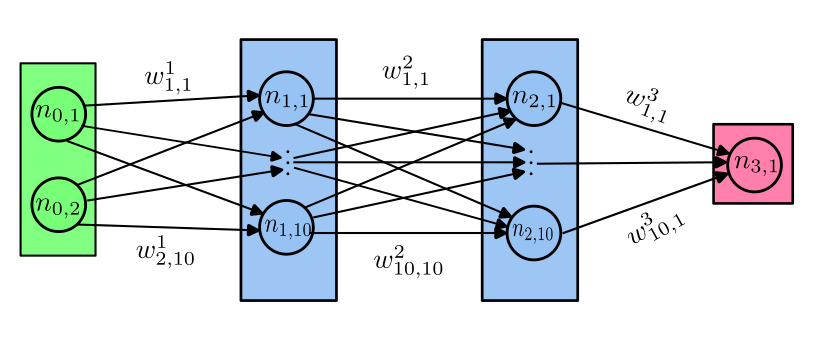
\includegraphics[width=1\linewidth]{Figures/neural_network.png}
    \caption{A feedforward neural network with 2 inputs, 2 hidden layers with 10 neurons each, and 1 output neuron. I use the notation $n_{lv}$ to represent neuron $v$ from layer $l$ and $w^l_{uv}$ to represent the weight from neuron $u$ in layer $l-1$ to the neuron $v$ in layer $l$.}
    \label{nn}
\end{figure}

\subsection{The Classification Problem}
Classification is a supervised machine learning method, in which training samples have class labels and the goal is to find a model such that the model performs well on new unseen test samples. In this thesis, I will work with binary classification, in which the model needs only to distinguish between two class labels, and multi-class classification, where the number of class labels is bigger than two. The most used loss function, or in LS terminology, objective function used to train NNs is the cross-entropy quantity, defined as:

\begin{align}
    \label{cross-entropy} H(P,Q) = -\mathbb{E}_{X \sim P} \log Q(x)
\end{align}
Intuitively, the cross-entropy measures the distance between two probability distributions, and in ML this is often used in gradient descent algorithms to minimize the loss. $P$ is the true probability distribution and $Q$ is the predicted. \\ 

\noindent Cross-entropy comes from information theory, but the cross-entropy quantity is actually also closely related to maximum likelihood estimation (MLE). If we denote the actual distribution of the training data by $p_{\text{data}}(\mathbf{x})$ and let $p_{\text{model}}(\mathbf{x}; \boldsymbol{\theta})$ be the probability distribution that tries to describe the actual distribution of the training data, then the goal is find $\boldsymbol{\theta}$, so that $p_{\text{model}}(\mathbf{x}; \boldsymbol{\theta})$ is as high as possible. Assuming that $m$ examples, $X = \{ x^{(1)}, \ldots, x^{(m)} \}$, are drawn, independently, from the true but unknown data generating distribution $p_{\text{data}}(\mathbf{x})$, the MLE estimator for $\boldsymbol{\theta}$ is defined as: 

\begin{align*}
    \boldsymbol{\theta}_{\text{ML}} &=  \underset{\boldsymbol{\theta}}{\arg \max} \;  p_{\text{model}} (X; \boldsymbol{\theta}) \\
    & = \underset{\boldsymbol{\theta}}{\arg \max} \; \prod_{i=1} ^m p_{\text{model}} (\mathbf{x}^{(i)}; \boldsymbol{\theta})
\end{align*}
where the rewriting is allowed because of the assumption of independence. This is known as the likelihood function. The goal is to maximize it, and by taking the logarithm of it, the arg max is not changed, but it transforms the product into a sum. 

\begin{align*}
    \boldsymbol{\theta}_{\text{ML}} = \underset{\boldsymbol{\theta}}{\arg \max} \; \sum_{i=1} ^m \log p_{\text{model}} (\mathbf{x}^{(i)}; \boldsymbol{\theta})
\end{align*}
The arg max does not change when rescaling, so dividing by $m$, we obtain a version of the estimate that is expressed as an expectation with respect to the empirical distribution, $\hat{p}_{\text{data}}$ defined by the training data:

\begin{align*}
    \boldsymbol{\theta}_{\text{ML}} = \underset{\boldsymbol{\theta}}{\arg \max} \; \mathbb{E}_{X \sim \hat{p}_{\text{data}}} \log p_{\text{model}} (\mathbf{x}; \boldsymbol{\theta})
\end{align*}
Maximizing this is equivalent to minimizing equation (\ref{cross-entropy}), where $p_{\text{model}}(\mathbf{x}; \boldsymbol{\theta})$ is the predicted probabilities and $\hat{p}_{\text{data}}$ is the true probability distribution. Normally in supervised learning, we are interested in the case of predicting $\mathbf{y}$ given $\mathbf{x}$, so the goal is to estimate the conditional probability $P(\mathbf{y} \mid \mathbf{x}; \boldsymbol{\theta})$. Denoting by $\mathbf{X}$ all the inputs and $\mathbf{Y}$ all the targets, then the conditional MLE estimator is:

\begin{align*}
    \boldsymbol{\theta}_{\text{ML}} &= \underset{\boldsymbol{\theta}}{\arg \max}P(\mathbf{Y} \mid \mathbf{X}; \boldsymbol{\theta}) \\
    & = \underset{\boldsymbol{\theta}}{\arg \max} \; \sum_{i=1} ^m \log P (\mathbf{y} ^{(i)} \mid \mathbf{x}^{(i)}; \boldsymbol{\theta})
\end{align*}





\subsubsection{Binary Classification Example}
For binary classification, only a single neuron is needed in the output layer. Here the training samples can be labeled by '0' and '1' respectively and the preactivation value at the neuron in the output layer can then be used to calculate the probability that the training sample is labeled as '1', denoted by $\hat{y}$, and obviously the probability that it is labeled as '0' is then given by $1 - \hat{y}$\\
\noindent Suppose we are in a setting where we train a binary classifier and we have a training sample labeled '1', $y=1$, and its preactivation value at the output neuron is -2. We want to know what the binary cross entropy loss is. As a first step, we need to figure out what the probability of $y = 1$ is. To do this, we use the logistic function to get the predicted probability, $\hat{y}$:
\begin{align*}
    \hat{y} = \frac{1}{1 + \exp(-2)} \approx 0.1192 
\end{align*}
To get the loss, we use the formula from (\ref{cross-entropy}):
\begin{align*}
    H(P,Q) = - \sum_i p_i \log q_i = -y \log \hat{y} - (1-y) \log(1-\hat{y}) = - \log{0.1192} \approx 2.1269
\end{align*}
The loss is quite large since the correct label is '1', and the preactivation value is negative. In binary classification, whenever the label is '1', the preactivation value should be as large as possible to get the highest predicted probability. 

\subsubsection{Multi-class Classification}
The example and intuition above generalizes to multi-class classification, however now the number of neurons in the output layer need to be equal to the number of classes. In this case, we cannot use the logistic function anymore to get the predicted probability. Instead we take the vector of preactivation values from the output layer and apply the softmax function to it, which gives a vector of probabilities for each class such that the probabilities sum up to 1. Formally, given the vector $z$ with preactivation values, this is defined as: 

\begin{align}
    \label{softmax} \text{softmax} (\mathbf{z})_j = \frac{\exp(z_j)}{\sum_{k=1}^m \exp(z_k)}
\end{align}
where $m$ is the number of classes and the classes are labeled $1, \ldots, m$. The cross-entropy loss, is, however, easier to calculate in this case using (\ref{cross-entropy}), as this reduces to the negative of the logarithm of the probability for the right label:
\begin{align*}
    H(P,Q) = - \log \frac{\exp(z_y)} {\sum_{k=1}^m \exp(z_k)}
\end{align*}



\subsection{Traditional Neural Network Training}
Optimization algorithms within ML and DL differ from traditional optimization problems. In ML it is the goal to perform well on some unknown test set, which is in contrast to traditional optimization problems, where solving the problem at hand is the task. To measure the performance of a ML model, the model is tested on a held-out test set. This is used to estimate how well the model generalizes. It can be beneficial to divide the remaining training set into two disjoint sets - a final training set and a validation set. The validation set can be used during training for model selection or hyperparameter selection, but it is not used to train the main parameters of the model. The test set is not seen before after the entire training process and as such it is only seen once, while the validation set can be seen many times. \\ 

\noindent For classification, we are concerned about predicting as many samples in the test set correctly as possible. To evaluate a classification model a well-known performance measure is the 0-1 loss, which basically returns the error rate, however, this loss-function is not well-suited for optimization tasks neither in traditional NN training nor in a LS context. In traditional NN training, a surrogate loss function is used instead, which could be the cross-entropy loss function introduced earlier. Some reasons for this are that the 0-1 loss is non-differentiable, non-continuous and it does not give as robust a model as when using the cross-entropy loss function. To prevent overfitting, which occur when the training error is small, but the test error is large, it is possible to use an early stopping technique, where the model trained is tested at certain times on the validation set. Here it is often the 0-1 loss used and the model with the smallest loss is then chosen, even though a later model might have smaller loss when using the surrogate function. \\ 

\noindent The most common optimization algorithm within ML and especially DL is stochastic gradient descent (SGD). SGD works by sampling a small subset of samples from the training set. Sometimes this is referred to as a minibatch, but herein I will use the term 'batch'. The batch is then used to compute the gradients of the parameters and very small updates are made to the parameters. In algorithm \ref{sgd} pseudocode of a simple version of SGD can be seen. In practice, the convergence criterion is often replaced by iterating over the entire training set for a certain number of epochs and the learning rate, which is a very sensitive hyperparameter should decrease during the training. Many extensions of this, conceptually simple, algorithm exists. Some of these extensions try to overcome some of the challenges that arise when training NNs. To accelerate learning momentum can be introduced, or to overcome the problem of choosing the correct learning rate, algorithms with adaptive learning rates can be used, which however, introduce more hyperparameters. Early stopping can be applied by testing the model on the validation set after each time the entire training set has been seen, called an epoch. 

\begin{algorithm}
\caption{Pseudocode for Stochastic Gradient Descent} \label{sgd}
\begin{algorithmic}
    \State \textbf{Require:} Learning rate $\epsilon$ 
    \State \textbf{Require:} Initial parameter $\boldsymbol{\theta}$
    \While {Convergence criterion is not met}
        \State Sample a batch from the training set 
        \State Compute gradient estimate $\boldsymbol{\hat{g}}$
        \State Apply update: $\boldsymbol{\theta} \leftarrow \boldsymbol{\theta -} \epsilon \boldsymbol{\hat{g}}$
    \EndWhile
\end{algorithmic}
\end{algorithm}

\subsection{Binary Neural Networks}
% Evt. kilde til Hubara. 
The development in the use of NNs have pushed the limits of AI significantly, however, before the introduction of BNNs the NNs were trained using one or many GPUs. This means that it is a challenge to run NNs on low-power devices. BNNs are networks, where weights and activations are limited to be either -1 or 1. \cite{Hubara2016} showed that it was possible to train BNNs without suffering any loss in classification accuracy. They used the traditional gradient descent approach and then made several tricks to come up with a solution that handles the challenges of training BNNs in this way. Normally, the gradient update in Algorithm \ref{sgd} is based on the gradients found by backpropagation, but for BNNs the gradient of the sign function used to binarize the weights is zero almost everywhere. Instead they use an estimator for this gradient called the straigt through estimator. With their training approach, they compute the real-valued gradients during the backward pass, and only binarize during the forward pass. How to train BNNs using traditional GD methods have been an active research area and it is without the scope of this thesis to give a full overview. For a more comprehensive review, I refer to \cite{yuan2023}. 

\subsection{Ensemble Methods}
In ML, ensemble methods are powerful techniques that combine the predictions of multiple models to improve overall performance and robustness. Two of the most well-known ensemble methods are bagging and boosting. \\

\noindent Bagging, short for Bootstrap Aggregating, involves creating $k$ different datasets. Each dataset is constructed by randomly sampling from the original dataset with replacement. This process generates $k$ datasets, each containing duplicates of some examples while others are omitted. $k$ models are then trained on these different datasets, and their predictions are aggregated through voting, leading to a more stable and accurate final prediction. \\

\noindent Boosting, on the other hand, trains several models sequentially on the same dataset. The key idea is to assign weights to the training examples, adjusting them after each model is trained. If a model $i$ misclassifies certain examples, these examples are given higher weights for the training of model $i+1$. This ensures that the new model focuses more on the difficult cases, improving the overall performance. \\

\noindent In this thesis, I implement the BeMi ensemble introduced by \cite{ambrogio2023}. Given a set of classes $C$ in a classification problem, this ensemble trains $\binom{\vert C \vert} {2}$ different neural networks, each designed to distinguish between two distinct classes from $C$. The idea is to pass the inputs through all these networks. If all networks trained on the true label of the input classify it correctly, then at most $\binom{\vert C \vert - 1}{2-1} - \binom{\vert C \vert - 2}{2-2}$ other networks can misclassify the input, ensuring the ensemble's correct classification. \\

\noindent MNIST is a widely recognized dataset used for classifying handwritten digits ranging from 0 to 9. For this task, $\binom{10}{2} = 45$ binary classifiers are required, each trained to differentiate between pairs of digits. When a test example is classified, it is fed into all 45 networks. If all 9 networks that have encountered the test example's true label classify it correctly, then at most $\binom{9}{1} - \binom{8}{0} = 8 $ other networks can misclassify it, ensuring the correct prediction. A test example can also be classified correctly when two labels receive the same number of votes. In this case, the network trained to distinguish between these two labels is used to break the tie. If this network's prediction is correct, it also counts as a correct prediction.

\newpage
\section{Local Search Model for Binary and Ternary Neural Networks}

A local search (LS) algorithm starts from a solution, which may be a random assignment of values to the decision variables. From here it moves from the current solution to a neighboring solution in the hope of improving a function $f$. A solution is denoted by $s$, and the set of neighboring solutions of $s$, $N(s)$, is called the neighborhood of $s$. In the following I will define the LS model I have used to train BNNs and TNNs and explain how local search is used. 

\subsection{Notation}
A BNN is a network where the weights and activations are restricted to $\pm 1$, whereas allowing the weights to be equal to 0 gives a Ternary Neural Network (TNN). This model applies for fully connected NNs, where the input comes from the data. I denote by $N = \{N_0, N_1, \ldots, N_L\}$ the set of layers in the network where $N_0$ is the input layer and $N_L$ is the last layer. For each layer, the set of neurons are denoted by $N_l = \{1, 2, \ldots, n_l\}$ such that the width of layer $l$ is $n_l$. The decision variables are the weights between each layer. The weight between neuron $u$ in layer $N_{l-1}$ and neuron $v$ in layer $N_l$ is denoted by $w_{uv}^l$. For the hidden layers, the activation function used to binarize the output is given by: 

\begin{align}
    \label{act} p(x) = 2 \cdot \mathbb{I} (x \geq 0) - 1
\end{align}

\noindent The training set can be written as $TR = \{ (\mathbf{x}^1, y^1), \ldots , (\mathbf{x}^T, y^T) \}$ such that $\mathbf{x}^i \in \mathbb{R}^{n_0}$ and $y^i$ is the label of the instance $i$ for every $i\in \{1, 2, \ldots, T\}$. It is beneficial to keep track of the preactivation values for all training instances for all the neurons in the layers $\{N_1, \ldots, N_L\}$. I use $s_v^{il}$ to denote the preactivation for instance $i$ at neuron $v$ in layer $l$. Similarly, for all the hidden layers $\{N_1, \ldots, N_{l-1}\}$, the output of the activation is denoted by $u_v^{il} = p(s_v ^{il})$. 

\noindent All of the above can also be written in terms of matrices and vectors. The input matrix is then denoted by $X \in \mathbb{R}^{T \times n_0}$ such that every row corresponds to the input of a specific instance and $Y$ is a vector with the labels. Then the mathematical model for a BNN can be written as:

\begin{align}
    \label{obj} \max \;\quad  & f(S^L, Y) \\
    \label{c1} \mbox{s.t.}\quad  & U^0 = X \\
    \label{c2} & S^l = U^{l-1}W_l \quad \quad \quad \quad \quad \forall l \in \{1, \ldots, L\} \\
    \label{c3} & U^l = p(S^l) \quad \quad \quad \quad \quad \quad \forall l \in \{1, \ldots, L- 1\} \\
    \label{c4} & W^l \in \{-1, 1\}^{n_{l-1} \times n_l} \quad \quad \forall l \in \{1, \ldots, L\} \\
    \label{c5} & X \in \mathbb{R}^{T \times n_0}
\end{align}

\noindent where (\ref{act}) is applied elementwise. Notice that I maximize a function, which is in contrast to standard ML, where the crossentropy loss is often minimized. I overcome this by multiplying by $-1$, whenever I use a loss function that is tradtionally minimized. If the input is real-valued, then $S_1$ is also real-valued but because of the binary activations and weights, $S^l$ is integer-valued for $l\in \{2, \ldots, L\}$. For a TNN, 0 is included to be an option for the $W$-matrices. Occassionally I will also use the notation $S^l_v$, which is a vector of the preactivation values in layer $l$, but only for neuron $v$. 

\subsection{Solution Generation, Neighborhood and Move}

As earlier mentioned, the decision variables are the weights between the layers. The preactivations and activations are determined by the input data and the weights. The number of variables in the model are thus given by $k = n_0\cdot n_1 + n_1 \cdot n_2 + \ldots + n_{L-1} \cdot n_L$. This means that the number of possible solutions for a TNN is $3^k$ and for a BNN it is $2^k$. To generate a solution, I use a uniform, random assignment of the allowed values to the variables. I use a 1-exchange neighborhood such that the neighbors to a solution $s$ are the solutions $s'$ in which it is only a single weight that has another value. This gives a neighborhood of size $k$ for a BNN and $2k$ for a TNN. A move is thus defined as the operation that take a solution $s$ to a new solution $s'$ by changing the value of exactly one weight. For a BNN this is simply a 'flip' from -1 to 1 or from 1 to -1, whereas for a TNN there is always two new values that a weight can take. \\

Often the number of weights in a NN are very large, and even though I only work with relative small NNs the number of weights quickly grows large. As a result, I found it to be inefficient to implement a function that tests the effect of a single move. For this reason I developed another approach, in which I evaluate several moves at once. I will elaborate on this later with an example. 

\subsection{Objective Functions}
As discussed earlier, when training NNs surrogate loss functions are often used, because the performance measure one is often interested in is non-differentiable, non-continuous and it might not be flexible enough. From now on I will denote the function to be maximized as an objective function, and whenever this corresponds to a loss function, which are normally minimized, I simply multiply the objective function value by -1 to get a maximization problem. In ML the objective function is used to compute gradients, that can be used to update the parameters in a gradient descent algorithm. In a LS context, an objective function does not necessarily have to be differentiable. In my implementation I support three different type of objective functions.

\subsubsection{Cross Entropy Objective Function}
I have already introduced the cross entropy function earlier. As I have implemented everything as a maximization problem, the objective function becomes:

\begin{align}
    \label{cs} \max \sum_{i=1}^m \log P(\mathbf{y}^{(i)} \mid \mathbf{x}^{(i)})
\end{align}
where $m$ is the number of samples in the batch, $\mathbf{y}^{(i)}$ is the label of sample $i$ with input data $\mathbf{x}^{(i)}$. Since the probabilities are always between 0 and 1, and the logarithm takes each probability and map them to a value between $(-\infty, 0)$, the range of this objective function is $(-\infty, 0)$. 

\subsubsection{Integer Max Margin Objectice Function}
The cross entropy objective function work with real-valued numbers. It might be beneficial to work with an integer-valued objective function for memory effiency reasons. As such I propose what I call the Integer Max Margin objective function. It builds on exactly the same intuition as the others, which for the multiclassification problem is to maximize the preactivation value for the neuron corresponding to the correct label. As earlier let $i$ denote a training instance and let $y^i$ be the true label, and let $\hat{y}^i$ be the predicted value defined as:

\begin{align}
    \label{y_hat} \hat{y}^i = \max _{v\in \{1, \ldots, n_L \} } s_v^{iL}
\end{align}

\noindent The goal is to stay within integers and at the same time predict confidently. One way to do this is to maximize the distance between the true label and the label with highest preactivation value, corresponding to highest probability, that are not the true label. So if $\hat{y}^i \neq y^i$ then $s_{\hat{y}^i}^{iL} > s_{y^i}^{iL}$ and the contribution to the objective function in this case will be $s^{iL}_{y^i} - s_{\hat{y}^i}^{iL}$ which is negative. The first goal would then be to minimize the gap between the wrongly prediction and the true label. On the other hand, if $\hat{y}^i = y^i$, then the model predicts correctly and in this case the goal is to maximize the distance to the label that come closest. This term can be written as: $s_{y^i}^{iL} - \max_{v \in \{1, \ldots, n_L\} \setminus y^i } s_v ^{iL}$. This can be summarized into a single line, so that the objective function, for a single instance, is given by: 

\begin{align}
    \label{integer_objective} f(\mathbf{x}^i, y^i) = s_{y ^i} ^{iL} - \max_{v \in \{1, \ldots, n_L\} \setminus y^i } s_v ^{iL}
\end{align}
As a result, the objective function for all $m$ samples in a batch becomes:
\begin{align}
    \label{int} \max \sum_{i=1} ^m \big[ s_{y ^i} ^{iL} - \max_{v \in \{1, \ldots, n_L\} \setminus y^i } s_v ^{iL}  \big]
\end{align}

The range of this objective function is theoretically given by $[-m \cdot n_{L-1}, m \cdot n_{L-1}]$. 

\noindent For the binary classification problem, this does not work as there is only one neuron at the final layer. The bounds for the preactivation values are determined by the number of neurons in the second last layer, $n_{L-1}$, such that the bounds are given by $[-n_{L-1}, n_{L-1}]$. For binary classification problems, the labels can also be encoded as -1 and 1. For the samples labeled 1, the goal is to get the preactivation values as close to $n_{L-1}$ as possible, or equivalently, maximize the distance to $-n_{L-1}$. The goal is opposite for the samples labeled -1, here the goal is to get the preactivation values as close to $-n_{L-1}$ as possible. For a single instance, this can be summarized into:
\begin{align}
    \label{integer_objective_binary} f(\mathbf{x}, y) = y\cdot s^L + n_{L-1}
\end{align}
To see this, take the case of $y=1$, then we want to maximize $s^L - (-n_{L-1})$ which is equivalent to (\ref{integer_objective_binary}). On the other hand, if $y = -1$, then we want to maximize the distance from $s^L$ to $n_{L-1}$, which is the same as $n_{L-1} - s^L$. Again, when multiplying $s^L$ with $y$ this is equivalent to (\ref{integer_objective_binary}). For all $m$ samples, the objective function is thus given by:
\begin{align}
    \label{int_binary} \max \sum_{i=1} ^m \big[ y^i \cdot S^{iL} + n_{L-1} \big]
\end{align}

\subsubsection{Comparison Between Cross Entropy and Integer Objective Function}
To illustrate the difference between this objective function and the crossentropy, suppose we are in a setting with 5 different classes, the correct label is the first label and the preactivation values for the 5 neurons in the output layer is given by $[4, 2, -2, -2, -2]$, such that the contribution to the crossentropy objective function is $-0.133456$ (after multiplying by -1). The contribution to the integer objective function is 2. Clearly, we are most interested in decreasing the preactivation value for the neuron with value 2, as this would mean a more confident (and correct) prediction of our instance. However, suppose we find a move that decreases the preactivation value of the third neuron from -2 to -4. This gives a new contribution from the crossentropy function equal to $-0.131558$, which is only a very small improvement. On the other hand, this is not an improvement for the integer objective function, where an improvement only is found if either the preactivation value of the first neuron increases or the preactivation value for the second neuron decreases. 

\subsubsection{Brier Score}
So far I have introduced two objective functions, whose range is quite large. As I, later on, want to test whether it is possible to add a regularization parameter to the objective function to minimize the number of connections in a TNN, it is desirable to also have an objective function, which have a more constrained range. The Brier score, which measures the accuracy of probabilistic predictions, gives this possibility. For binary classification using 0-1 encoding of the labels, the Brier score is defined as: 

\begin{align}
    BS = \frac{1}{m} \sum_{i = 1} ^m (p(y^i) - y^i) ^2 
\end{align}
where $p(y^i)$ is the probability that $y^i$ is 1 and $y^i$ is the actual outcome. This corresponds to the mean squared error, and it gives a value between 0 and 1, where 0 is the best score achievable. I formulate it without taking the mean and convert it to a maximization problem by multiplying with $-1$, so the objective function for binary classification becomes:
\begin{align}
    \label{BS_binary} \max \sum_{i=1}^m - (p(y^i) - y^i) ^2 
\end{align}
The range of this objective function value is $(-m, 0)$. \\
\noindent For the multiclassification task, the original BS score is defined by: 
\begin{align}
    BS = \frac{1} {m} \sum_{i=1} ^m \sum_{t=1} ^C (p(y^{ti}) - y^{ti})
\end{align}
where $C$ is the number of classes, $p(y^{ti})$ is the predicted probability for class $t$ for instance $i$. $y^{ti}$ is 1 of instance $i$ belongs to the $t$-th class and zero otherwise. Here the range is double, from zero to two. In my implementation I use:
\begin{align}
    \label{BS} \max \sum_{i=1}^m \sum_{t=1} ^C - (p(y^{ti}) - y^{ti})
\end{align}
The range of this objective function is thus $(-2m, 0)$. 
\subsubsection{Minimizing the number of connections}
In a TNN it is possible to add a second term to the objective function measuring how many active connections are in the model, i.e. how many weights are not zero. The idea is, that the model should be as simple as possible to avoid overfitting. In this context simple means having fewer active connections. Thus, the goal of the second objective term is to minimize the number of connections. As I am working with maximization, the second objective term would look like this:

\begin{align}
    \label{min_connections}  - \alpha \sum_{l\in{1, \ldots, L}} \sum_{u \in N_{l-1}} \sum_{v \in N_l}  \text{abs}(w^l_{uv})
\end{align}

\noindent where $\alpha$ is a weight used to penalize the number of connections. The term is negative as it is put into an maximization problem. The choice of $\alpha$ depends on the objective function it is used in, as the weighting of this second term should depend on what values the first term is taking. As such the Brier score objective function is an ideal choice to use in combination with this term, as the value of that is constrained. As an example suppose the number of training samples is given by $T = 1000$ and the number of weights in the neural network is 10000. Assume it is a multiclassification task. Then the objective function value for the Brier score is in the interval $(-2000, 0)$ and the second term would be in the interval $[-10000, 0]$, with $\alpha = 1$ that is. The total objective function value is as a result in the interval $(-12000, 0)$. A too high value of $\alpha$ would simply put all weight values to zero, but at the cost of predicting correctly. But a small value of $\alpha$, say $0.001$ would make the second term to be in the interval $[-10, 0]$, and it would no longer be beneficial to set all weights equal to zero at the cost of predicting correctly. 

\subsection{Delta Evaluation}
A very important part of a LS algorithm is how to select moves to commit to a solution. Often this is done by selecting a possible move, evaluating that move and get its delta value, which is a value telling how the objective function value is affected by that move. Afterwards a threshold value is used to determine if that move should be accepted or not. For maximization problems, the threshold value could simply be that the delta value should be above 0 in order for the move to be accepted. A critical function in a LS algorithm is thus the function that evaluates a move, as this is something that is done many times throughout the solution search. I found it to be highly inefficient to work with a function that evaluates only a single move. As the solution improves, more and more moves need to be tried before finding an improvement and a function that only evaluate a single move is too slow for this. Also, I found that by evaluating several moves, in a structured way, I found several tricks that speed up the evaluation. \\

The way I evaluate moves is by selecting a neuron in the neural network with weights going into it, so I do not select neurons from the input layer. For this neuron I evaluate the possible moves for the weights going into it. This is done simultaneously, but still independently in the way that I am testing what would happen if a single weight changes value, not what would happen if all of them change values at once. After this evaluation, a sequence of moves will be returned, each with their own delta value, that I can then use to determine what move to take. I will now introduce the most important aspects of this and will with an example show how it works. 

\subsubsection{Critical Samples}
Recall the binary activation function defined in (\ref{act}). The input to that function is the preactivation values, $s_v^{il}$ and in a LS context where only one-exchange moves are considered, there are values of these preactivation values such that the output of (\ref{act}) is unchanged regardless which of the weights going into neuron $v$ at layer $l$ change values. The weights can only take on values -1, 1 (0 as well for a TNN), so they can only change their value by either -2 or 2 in a BNN where -1 and 1 are also possibilities in a TNN. Thus, if we denote the maximum output value, or activation value, (in absolute value) from the previous layer by $u^{l-1}_{\max}$, then we can define the set of critical samples for a neuron, which are those samples that can change activation value by making a single move for one the weights going into that neuron, by:
\begin{align}
    \label{critical} \text{critical }^l_ v = \{ i \in \{1, \ldots, T\}: s_v^{il} \geq -2 \cdot u^{l-1}_{\max} \wedge s_v^{il} < 2 \cdot u^{l-1}_{\max} \}
\end{align}
I use a general notation to both describe the case for the first hidden layer, where the output from the previous layer are dependent on the input, but from the second hidden layer, it is possible to skip the $u^{l-1}_{\max}$ term, as this is equal to 1 as a result of the binary activation function. The purpose of these 'critical' samples, is that it greatly reduces the number of instances for which the delta evaluation need to be evaluated for. This trick is only used for the hidden layers, as the same does not apply for the output layer. 

\subsubsection{Forward Propagation}
The next trick that is useful when evaluating moves for a neuron is that it can be used to reduce the number of forward propagations. This logic applies both for a hidden layer and the output layer. It is a bit more complicated for the output layer in the TNN case, but nevertheless it is very useful. After having found the critical samples for a neuron (in a hidden layer), we need to evaluate what would happen if a move was applied to the weights going into the neuron. A naive way to do this would be to apply a forward propagation for all of the weights on the critical samples to see what would happen with the objective function value. But the binary activation function gives a way to do this more efficiently. The only way that something changes for a specific instance is if the activation of that instance changes, in which case we know that it changes it value by -2 or 2, dependent on the value of it before. Thus, we can simulate what would happen if the activations change for all the critical samples and find their 'delta changes' by doing a single forward propagation. Afterwards we can, for each weight we want to calculate the effect of a move for, find out if making the move would change the activations and then the 'delta changes' can be looked up instead of calculating it again. \\

\noindent For the output layer, a similar logic applies. Again a neuron is selected, but this time the critical set is not relevant, as the binary activation function is not used here. But again, for a BNN exactly one of two things happen (assuming the presence of at least one hidden layer): either the preactivation value increases by 2 or it decreases by 2. This comes from the fact that the output from the previous layer is either -1 or 1 and the value of the weight changes by either -2 or 2. Thus, it is again possible to find the 'delta changes' for the samples by simulating what would happen if their values increase by 2 and what would happen if they decrease by 2. Afterwards, for each single weight it can quickly be determined which of the cases a sample is in and the effect can be looked up in the 'delta changes'-tables. This greatly reduces the number of times the function calculating the objective function value needs to be called. For a TNN, it is almost the same, except 4 'delta changes'-tables are needed as the values can also increase and decrease by 1 in this case. 

\subsubsection{Example of Delta Evaluation}
To illustrate how the mechanisms described above works, I have constructed a BNN with the following structure $[784, 4, 4, 4, 10]$. I am training it on a balanced training set of 10 instances from the MNIST dataset. Initially I initialize a solution by randomly assigning values to all the weights and I am now looking for what move to make in order to improve the current solution. Suppose now that I look at the fourth neuron in the second hidden layer. The preactivations are given in the vector:

\begin{align*}
    S_4^2 = 
    \begin{bmatrix}
        0 & 4 & 4 & 2 & 2 & 2 & 4 & 2 & -2 & 2
    \end{bmatrix}
\end{align*}
Each element corresponds to a different training sample. Since we are in the second hidden layer, $u^1_{\max} = 1$ and thus $\text{critical }_4 ^2 = \{1, 9\}$, as it is only the instances with 0 and -2 as preactivation values that can change activation. Thus, for the remainder of the delta evaluation process for this neuron, it is only necessary to look at these two instances. The first thing needed to do is to simulate what would happen if their activations change. Thus, I start by calculating the effect of this by propagathing through the network. During the process, I always try to do as little work as possible meaning that whenever I can benefit from using the values already stored I do so. The preactivation values for the next layer for these two instances is currently given by:

\begin{align*}
    S^3 = 
    \begin{bmatrix}
        -2 & 0 & -2 & 0 \\
        -2 & 0 & -2 & 0 
    \end{bmatrix}
\end{align*}
where each row corresponds to an instance and each column to a neuron at the next layer. The weight vector going into the next layer from the fourth neuron in the second layer is given by:
\begin{align*}
    W = 
    \begin{bmatrix}
        -1 & 1 & 1 & 1
    \end{bmatrix}
\end{align*}
Looking at the critical instances it is easy to recognize, that if they changed sign and thus activation, then the first would decrease from 1 to -1 and the second would increase from -1 to 1. Thus, we have:
\begin{align*}
    \hat{S}^3 = S^3 + 
    \begin{bmatrix}
        -2 \\
        2
    \end{bmatrix}
    \circ 
    \begin{bmatrix}
        -1 & 1 & 1 & 1 
    \end{bmatrix}
    = 
    \begin{bmatrix}
        0 & -2 & -4 & -2 \\
        -4 & 2 & 0 & 2 
    \end{bmatrix}
\end{align*}
Here $\circ$ is elementwise mulplication. \\
\noindent Until now it has been possible to calculate what is happening by looking at the preactivation values stored in memory and updating them. This is efficiently to do for the neuron that is being evaluated and for the next layer, but afterwards it makes more sense to forget what is in memory and instead finish the forward propagation with the temporary matrices. To finish the forward propagation one need to apply the activation function, (\ref{act}), to $\hat{S}^3$, yielding the result: 
\begin{align*}
    \hat{U}^3 = 
    \begin{bmatrix}
        1 & -1 & -1 & -1 \\
        -1 & 1 & 1 & 1 
    \end{bmatrix}
\end{align*}
The last step is to multiply with the last weight matrix to obtain the preactivation values for the last layer. Here I will only give the result:
\begin{align*}
    \hat{S^4} = \hat{U^3}W^4 = 
    \begin{bmatrix}
        2 & 0 & 0 & -4 & 4 & 2 & -2 & 2 & 0 & 2 \\
        -2 & 0 & 0 & 4 & -4 & -2 & 2 & -2 & 0 & -2
    \end{bmatrix}
\end{align*}
Compare this to the current preactivation values, which is determined after the random initialization:
\begin{align*}
    S^4 = 
    \begin{bmatrix}
        -4 & -2 & 2 & 2 & -2 & 0 & 0 & 0 & -2 & -4 \\
        -4 & -2 & 2 & 2 & -2 & 0 & 0 & 0 & -2 & -4
    \end{bmatrix}
\end{align*}
Since the correct labels for these two instances are 4 and 9 respectively (using 0-indexing), the objective vector, using the integer objective function, is initially given by:
\begin{align*}
    O = 
    \begin{bmatrix}
        -2 - 2 \\
        -2 - 4 
    \end{bmatrix}
    = 
    \begin{bmatrix}
        -4 \\
        -6 
    \end{bmatrix}
\end{align*}
whereas using $\hat{S}^4$, the result is:
\begin{align*}
    \hat{O} = 
    \begin{bmatrix}
        4 - 2 \\
        -4 -2 
    \end{bmatrix}
    = 
    \begin{bmatrix}
        2 \\
        -6 
    \end{bmatrix}
\end{align*}
This gives a vector of delta changes:
\begin{align*}
    D = \hat{O} - O = 
    \begin{bmatrix}
        2 - (-4) \\
        -6 - (-6) 
    \end{bmatrix}
    = 
    \begin{bmatrix}
        6 \\ 
        0 
    \end{bmatrix}
\end{align*}
This means that we have found out that if the activations change for the two critical instances, then this has a positive effect for one of them and zero effect for the other. The last thing we need to do is to find out which, if any, of the four weights going into the neuron can make the activations change. The current weights going into this neuron has the values: 
\begin{align*}
    W_4^2 = 
    \begin{bmatrix}
        -1 & 1 & 1 & 1
    \end{bmatrix}
\end{align*}
and the output of the previous layer for the two critical instances are:
\begin{align*}
    U^1 = 
    \begin{bmatrix}
        1 & -1 & 1 & 1 \\
        1 & -1 & -1 & 1
    \end{bmatrix}
\end{align*}
What I then do is that I create four copies of the preactivation values for the critical instances, one for each weight going into the neuron. Afterwards I simulate what would happen if the weights are 'flipped', take the activations of these simulated preactivation values and compare them to the current activations. This gives me a matrix where each row represents an instance and the column represents a weight. The elements indicate whether the activation has changed or not, meaning that to get the effect of a weight we can columnwise take the inner product between the column and the delta changes vector, $D$, found earlier. I start by finding the simulated preactivation values:
\begin{align*}
    \hat{S}^2_4 = 
    \begin{bmatrix}
        0 & 0 & 0 & 0 \\
        -2 & -2 & -2 & -2
    \end{bmatrix}
    + 
    \begin{bmatrix}
        1 & -1 & 1 & 1 \\
        1 & -1 & -1 & 1
    \end{bmatrix}
    \circ 
    \begin{bmatrix}
        2 & -2 & -2 & -2
    \end{bmatrix}
    =
    \begin{bmatrix}
        2 & 2 & -2 & -2 \\
        0 & 0 & 0 & -4
    \end{bmatrix}
\end{align*}
I then need to find out where there is a change in activation values compared to the current solution. Clearly, since the current preactivation value for the first instance is 0, this activation is currently 1, and for the second it is -1 as the preactivation value is -2. Thus, it gives the following 'changes' matrix, where 1 indicate that the activation has changed and 0 indicate that it has not. 
\begin{align*}
    \text{changes} = 
    \begin{bmatrix}
        0 & 0 & 1 & 1 \\
        1 & 1 & 1 & 0
    \end{bmatrix}
\end{align*}
As an example this shows that for the weight indexed by the third column, flipping that value from 1 to -1, will change the activation of both the critical instances. The last remaining thing to do is to, columnwise found the effect of flipping each weight. This gives the following delta values:
\begin{align*}
    DW = 
    \begin{bmatrix}
        0 \cdot 0 + 1 \cdot 0 & 0 \cdot 0 + 1 \cdot 0 & 1 \cdot 6 + 1 \cdot 0 & 1 \cdot 6 + 0 \cdot 0
    \end{bmatrix}
    = 
    \begin{bmatrix}
        0 & 0 & 6 & 6
    \end{bmatrix}
\end{align*}
Thus, an improvement of 6 in terms of the integer objective function can be found by flipping the third or fourth weight going into this neuron. 





\subsection{Solution Improvement}
Recall, that the goal of the classification problem is to be able to classify test samples that are not seen during training. During training, the model is trained on batches of training samples, and an objective function is used to evaluate the quality of the model. I will test the effect of using a single batch compared to using several, and a key ingredient in most of my algorithms is the iterated improvement algorithm. In words, this algorithm takes a solution and searches for improvements. I do this by iterating through the neurons in the network as described earlier. For each neuron, it takes the best move found and checks whether this is an improvement, and if it is, the move is committed and the current solution is updated. The algorithm only stops when the time limit has been reached or the solution has reached a local optima, which is when all the neurons have been checked without finding an improvement. In practice, it is quite fast to end up in a local optima for a single batch. The pseudocode for this algorithm can be seen in Algorithm \ref{iterated_improvement}. \\

\begin{algorithm}[!tb]
    \caption{Pseudocode for Iterated Improvement} \label{iterated_improvement}
    \begin{algorithmic}[1] 
        \State \textbf{Input:}
        \State \hspace{\algorithmicindent} Initial solution $currentSolution$
        \State \hspace{\algorithmicindent} Time limit $timeLimit$
        \State $startTime \gets$ current time
        \While{current time $-$ $startTime < timeLimit$}  
            \State Shuffle the nodes of $currentSolution$
            \State $improvementFlag \gets \text{False}$
            \For{each $node$ in $currentSolution$}
                \State $bestMove \gets$ findBestMove($currentSolution$, $node$)
                \If{delta value of  $bestMove > 0 $}
                    \State $currentSolution \gets $ applyMove($currentSolution$, $bestMove$)
                    \State $improvementFlag \gets \text{True}$
                \EndIf
                \If{current time $-$ $startTime \geq timeLimit$}  
                    \State \textbf{return} $currentSolution$
                \EndIf
            \EndFor
            \If{$improvementFlag = \text{False}$}  
                \State \textbf{return} $currentSolution$
            \EndIf
        \EndWhile
        \State \textbf{return} $currentSolution$
    \end{algorithmic}
\end{algorithm}

\noindent Using only Algorithm \ref{iterated_improvement} will typically not yield good results. While training a neural network, many local optima are usually visited, and traditional neural network training has several techniques to escape from a local optima. I will use a simple optimization metaheuristic, iterated local search (ILS), to escape from the local optima. This metaheuristic works by taking the current solution, which is a locally optimal solution, and use it to get another solution, which is no longer locally optimal. Afterward, iterated improvement will be applied to the new solution until it arrives at a local optima and the process repeats itself until the solution has converged or the time limit has been reached. The strategy used to get another solution from the current solution is called perturbation. In the context of training BNNs and TNNs, it works by taking a solution and randomly changing the values of a number of the weights. The important parameter here is how many weights to change values of. If too few weights are changed, there is a high chance that the solution falls back to the same local optima it came from. On the other hand, if too many weights are changed, it could be the same as using random restart, which could mean that the solution quality does not improve much. The pseudocode is given in Algorithm \ref{ils}. \\

\noindent Another problematic aspect of this algorithm is that it is more difficult to determine when the model has converged. Instead of a convergence criterion, I use a time limit, such that the runtime is controlled. A convergence criterion could be to set a maximum number of perturbations allowed without ending up in a local optima that is better than the best seen so far. 

\begin{algorithm}[!tb]
    \caption{Pseudocode for Iterated Local Search} \label{ils}
    \begin{algorithmic}[1]
        \State \textbf{Input:}
        \State \hspace{\algorithmicindent} Initial solution $currentSolution$
        \State \hspace{\algorithmicindent} Time limit $timeLimit$
        \State \hspace{\algorithmicindent} Perturbation size $ps$
        \State $startTime \gets$ current time 
        \State $bestSolution \gets currentSolution$ 
        \While{current time $-$ $startTime < timeLimit$}
        \State $currentSolution \gets$ IteratedImprovement($currentSolution$,
        \Statex \hspace{\algorithmicindent} \hspace{\algorithmicindent}$timeLimit$ - (current time - $startTime)$)
        \If{$currentSolution$ $>$ $bestSolution$}
            \State $bestSolution \gets currentSolution$ 
        \ElsIf{$currentSolution < bestSolution$}
            \State $currentSolution \gets bestSolution$ 
        \EndIf
        \State $currentSolution \gets$ Perturb($currentSolution$, $ps$)
        \EndWhile
        \If{$currentSolution > bestSolution$}
            \State \textbf{return} $currentSolution$
        \Else 
            \State \textbf{return} $bestSolution$
        \EndIf
    \end{algorithmic}
\end{algorithm}

\subsection{Multiple Batch Training}

One of the ways I try to make sure that the models trained generalize well is to make use of more data and train the network on several batches. It is the same solution that is being trained on all of the batches, in the sense that the solution after training one batch is the starting solution to the next batch. This gives rise to a couple of problems. The first one is, how do we know what the 'best' solution is? If the solution returned is the one after the last batch, then it might be that it is heavily influenced by the last batch and as such it would have been better to use one of the solutions earlier on. Another consideration is how to make sure that the solution does not forget what it has learned from the previous batch. My attempt to solve these problems is to use an early stopping technique, where I after every $k$ batches get the validation accuracy on the validation dataset and after the complete training process I return the solution with the best validation accuracy. Of course, this introduces another parameter, $k$. Ideally one could set $k=1$ and get the validation accuracy for all the solutions, but this might be too costly as getting the validation accuracy involves evaluating the solution on a large dataset. \\

\noindent One of the concerns by training a model on several batches of data is that the model overfits on the batch it is currently trained on and forgets what it learned from the previous batch. For this reason, I investigate whether a sporadic local search approach helps the model to generalize better. This works by setting a parameter $bp$, which is a parameter in the interval $[0,1]$, which is given to the Bernoulli distribution, which then returns a '1' with probability $bp$ and a 0 otherwise. Before training on a batch, each weight samples a value from this distribution, and if the value is 1, then the weight is a part of the search for that batch and otherwise the value is kept fixed for that particular batch. For each new batch, new weights are selected to be part of the search. The hope is that this helps the model to avoid getting too focused on the current batch and reduce the overfitting gap. \\

\noindent The pseudocode for this algorithm is given in Algorithm \ref{multiple_batches}. In line 15 I give an additional parameter compared to the iterated improvement pseudocode in Algorithm \ref{iterated_improvement}. In practice it works a bit different, but this is just to underline that not all weights are part of the search. Notice, that this could easily be adjusted to using Algorithm \ref{ils} instead in line 15. The only difference would be that the algorithm needs to take a perturbation size as input and that each ILS phase are given a fixed time limit instead as it would continue indefinetely otherwise. 

\begin{algorithm}[H]
    \fontsize{12pt}{12pt}\selectfont
    \caption{Pseudocode for Multiple Batch Iterated Improvement} \label{multiple_batches}
    \begin{algorithmic}[1]
        \State \textbf{Input:}
        \State \hspace{\algorithmicindent} Time limit $timeLimit$
        \State \hspace{\algorithmicindent} Set of batches $batches$
        \State \hspace{\algorithmicindent} Interval to early stopping $k$
        \State \hspace{\algorithmicindent} Number of epochs $epochs$
        \State \hspace{\algorithmicindent} Bernoulli parameter $bp$ 
        \State $startTime \gets$ current time 
        \State $currentSolution \gets$ random solution
        \State $bestSolution \gets currentSolution$
        \State $bestValidationAccuracy \gets$ ValidationAccuracy($currentSolution$)
        \State $counter \gets 0$
        \While{current time $-$ $startTime < timeLimit$} 
            \For{$epoch$ in range($epochs$)}
                \For{$batch$ in $batches$}
                    \State $searchWeights \gets$ SelectWeights($bp$)
                    \State $currentSolution \gets$ IteratedImprovement($currentSolution$,
                    \Statex \hspace{\algorithmicindent} \hspace{\algorithmicindent}$timeLimit$ - (current time - $startTime)$, $searchWeights$)
                    \If{$counter$ modulo $k$ $ = 0$}
                        \State $ValidationAccuracy \gets$ ValidationAccuracy($currentSolution$)
                        \If{$ValidationAccuracy > bestValidationAccuracy$}
                            \State $bestSolution \gets currentSolution$ 
                            \State $bestValidationAccuracy \gets ValidationAccuracy$ 
                        \EndIf
                    \EndIf
                    \State $counter \gets counter + 1$
                    \If{current time $-$ $startTime \geq timeLimit$}  % Time check within loop
                        \State \textbf{return} $bestSolution$
                    \EndIf
                \EndFor
                \State $batches \gets$ ResampleBatches 
            \EndFor
        \EndWhile
        \State \textbf{return} $bestSolution$
    \end{algorithmic}
\end{algorithm}

\noindent So far I have looked at algorithms making moves based on one batch and tried to make sure that the model does not forget what it has learnt from other batches by only looking at a subset of the weights. An alternative method is to make less moves, but making sure that the moves generalize better. One possibility for this is to sum up delta values for the moves across several batches and only after a certain number of batches, some moves are committed. This should make sure that the moves committed benefit not only a single batch of samples, but multiple batches. An important decision to make is when to make updates. The more batches seen before making updates, the more confident will the algorithm be that the moves generalize well, but it will also be slower. For this reason I add another aspect to the algorithm, such that it initially make updates based on very few batches and later on it makes updates on more batches. The parameters for this are given in line 5-7 in Algorithm \ref{multiple_batches_v2}, which shows the pseudocode for this algorithm. \\

A problematic aspect of this algorithm is that the delta values are calculated under the assumption that a single move is taken, but here, to speed up the process, I take many moves at once. However, to avoid the moves interfering too much with each other I only take one move per neuron. A different problem is again the convergence problem, where I, to overcome this problem, use a time limit. For this algorithm I do not use early stopping as the use of several batches to make updates should make sure that it generalizes better compared to the version introduced earlier. 


\begin{algorithm}[H]
    % \footnotesize
    \fontsize{12pt}{12pt}\selectfont
    \caption{Pseudocode for Multiple Batch Aggregation Algorithm} \label{multiple_batches_v2}
    \begin{algorithmic}[1]
        \State \textbf{Input:}
        \State \hspace{\algorithmicindent} Time limit $timeLimit$
        \State \hspace{\algorithmicindent} Set of batches $batches$
        \State \hspace{\algorithmicindent} Bernoulli parameter $bp$ 
        \State \hspace{\algorithmicindent} How many batches before making updates in the beginning $updateStart$
        \State \hspace{\algorithmicindent} The maximum number of batches before making updates $updateEnd$
        \State \hspace{\algorithmicindent} How often to increase the update interval $updateIncrease$
        \State $startTime \gets$ current time 
        \State $currentSolution \gets$ random solution
        \State $updateInterval \gets$ $updateStart$
        \State $counter, \; updateCounter \gets 0, \; 0$    
        \State $searchWeights \gets$ SelectWeights($bp$)
        \State $deltaValues$ $\gets$ $0$
        \While{current time $-$ $startTime < timeLimit$}
            \For{$batch$ in $batches$}
                \State $updateCounter \gets updateCounter + 1 $
                \State $deltaValues \gets deltaValues$ + 
                \Statex \hspace{\algorithmicindent} \hspace{\algorithmicindent} CalculateDeltaValues($currentSolution$, $batch$, $searchWeights$)
                \If{$updateCounter = updateInterval$}
                    \For{each $node$ in $currentSolution$}
                        \State $bestMove \gets$ findBestMove($deltaValues$, $node$)
                        \If{delta value of  $bestMove > 0$}
                            \State applyMove($currentSolution$, $bestMove$)
                        \EndIf
                    \EndFor
                    \State $updateCounter \gets 0$ 
                    \State $deltaValues$ $\gets$ $0$
                    \If{$counter$ modulo $updateIncrease$ $ = 0$}
                        \State $updateInterval \gets updateInterval + 1$ 
                    \EndIf
                \EndIf
                \State $counter \gets counter + 1$
            \EndFor
            \State $batches \gets$ ResampleBatches 
        \EndWhile 
        \State \textbf{return} $bestSolution$
    \end{algorithmic}
\end{algorithm}





\subsection{Code Organization}

One of the major challenges of this thesis has been to develop the framework for training BNNs and TNNs. The framework needed to be quite flexible so that it allows both BNNs and TNNs, but also ensures that all of the algorithms and experiments can be tested within the same framework. All of the source code for this thesis can be found at: https://github.com/mbruh19/Master-Thesis. The implementation is done in Python. To train a BNN or TNN, 'main.py' needs to be called with the right parameters. From this file, everything else runs automatically. As a starting point, it initializes the 'Reader' class and loads the training, validation, and testing sets by calling the load data function. The current framework supports loading the MNIST, Fashion-MNIST (FMNIST) and the Adult dataset. To load from other datasets, the necessary function needs to be implemented in the Reader class. Next, the 'Instance' class is called, which takes all the settings of the experiment as input as well as the three datasets. The Instance class has the very important 'loader' function, needed to iterate through batches from one of the datasets. \\

\noindent Having this, one of the algorithms presented is called. When an algorithm is called, it initially starts by loading a batch and creating a 'Solution' object. This object is the core of the implementation. The most important attributes of this object are the $W$, $S$ and $U$ matrices introduced earlier as well as a vector, $O$ denoting the contribution of each sample to the objective function. It also has an attribute of the nodes in the network, that can be iterated through. The $S$, $U$ and $O$ attributes are dependent on the current batch, and as a result, the Solution object has a function to change the batch, which includes re-evaluating these attributes. The object also has functions to initialize a random solution and copy the weights. More importantly, it is also here the function to commit a move is located, where the necessary updates are done. The remaining functions are those to perturb the solution, used in ILS, and a function to select search weights, used in sporadic local search. \\

\noindent The algorithm then moves on and calls one of the 'solvers' implemented. There are two 'solvers' implemented, iterated improvement, which follows Algorithm \ref{iterated_improvement} or iterated local search, described in Algorithm \ref{ils}, which uses Algorithm \ref{iterated_improvement}. In the iterated improvement algorithm, the 'Delta Manager' object is called. This object has a single function, delta calculation, which either uses a delta function for BNN or TNN. This function takes the current solution and a node as input. For this node, all the weights going into this node, which are part of the search, are tested to see what the delta value is if the weight changes value. This follows the procedure described in section 5.4. The delta calculation function returns a sequence of moves back to the iterated improvement algorithm, which takes the best of the moves and decides whether to commit the move or not. If the algorithm uses multiple batch training, it loads a new batch, changes the batch on the solution object. and the process repeats itself until the time limit has been reached. \\

% Here I plan to include the following:

% \begin{itemize}
%     \item Intro to Local Search
%     \item Neighborhood
%     \item Local Search Algorithms - iterative improvement, first improvement, best improvement, random improvement
%     \item Local Search Metaheuristics - iterated local search 

% \end{itemize}
\newpage
\section{Experimental Analysis}

I have implemented several algorithms and each algorithm is dependent on different parameters, which makes it difficult to conduct a one-factor-at-a-time analysis. Instead, I try to be as structured as possible to test which algorithm, objective function, network structure, and network type (BNN or TNN) works best. 
I divide the experimental analysis into several sections. First I only test on the well-known MNIST dataset, which is a large database of handwritten digits. The dataset contains 60,000 training images and 10,000 testing images. Each image is a $28 \times 28$ grayscale image of a handwritten digit. At the end of the experimental analysis, I take the knowledge gained about which parameters work best for MNIST and try to see how they work on different datasets. The first section will concentrate on single batch training, which is relevant in few-shot learning. Here, the goal is to test which objective function works best, how the amount of data influences the accuracy, and the effect of the network size. This section will only use the ILS algorithm outlined in Algorithm \ref{ils}. Some of the network architectures tested will be identical to those of \cite{icarte2019} and \cite{thorbjarnason2023}, so a comparison can be made. At the end, a small hyper-parameter study will be conducted to see how sensitive the algorithm is to the choice of $ps$. \\

\noindent The second section is about multiple batch training. Again, the goal is to investigate which objective function works best, but the goal is also to test which of the two algorithms presented for multiple batch training works best. A focus point will also be how the algorithms scale with increasing network size. 
The first two sections will only deal with BNNs. In the third section, I will test the TNN, where I speficially aim to investigate whether a regularization parameter helps. Another focus point will be how it compares against a BNN, especially whether it requires more training time to obtain similar accuracies or not. 
In the fourth section, I present the results on the BeMi ensemble introduced by \cite{ambrogio2023}. Here, the focus will be on how the ensemble works with increasing amounts of training data, as this is a limitation for their MIP implementation. Finally, in the fifth section, I to use the knowledge obtained from the previous four sections to test how the best found algorithms and parameters generalize to other datasets. \\

\noindent The source code for the implementation in Python and experiment scripts can be found at: https://github.com/mbruh19/Master-Thesis. For all the experiments, the results reported are an average of 5 runs for each configuration tested. The experiment is run on a Windows 10 computer with a 64-bit operating system with 8 GB RAM. The processor is an Intel(R) Core(TM) i5-6400 CPU with 2.70GHz. 


\subsection{Single Batch Training}

This section will only use the ILS procedure presented in Algorithm \ref{ils}. In each perturbation, I initially change the value of 25 randomly chosen weights. The first goal is to explore which objective function works best under different circumstances. The first experiment will be to test the influence of more training data, but with a short time limit of only 60 seconds. The second experiment tests how the results change if the time limit is increased. In experiment 3, I test different network architectures, and finally, in experiment 4, I test how sensitive the results are to the choice of $ps$. For all the experiments in this section, to compare them against existing literature, I use a balanced training and test set meaning that the number of instances is equal for each class. The test accuracy is reported on a set of 8,000 instances from the test set, 800 instances for each digit.

\subsubsection{Comparing Objective Functions}

As a starting point, I begin by testing how the different objective functions compare with each other. The network has a single hidden layer, such that the network structure is $[784, 16, 10]$. I use a BNN with a time limit of 60 seconds. Besides comparing the objective functions with each other, I also want to see how the results develop as the amount of training data increases and to see, this I let the total number of training samples vary from 100 to 2000, or from 10 to 200 examples from each class. In Figure \ref{SBT_COF} I plot the mean of the test accuracy, with the standard deviation as a shaded area around it. Initially, as more training samples are added, the accuracy increases significantly, but later on the effect tapers off, and the accuracy actually decreases at the end for two of the objective functions. It is possible that the results could be even better with more time, which will be explored in the next experiment. Initially, the cross-entropy objective function works best, but eventually the integer objective function takes over. The objective function based on the Brier score does not seem to be able to compete with the other objective functions. The maximum mean accuracy achieved for this result is with the integer objective function and a batch size of 1800, which gives a mean accuracy of 71.73 \%. \\

\begin{figure}[!tb]
    \centering
    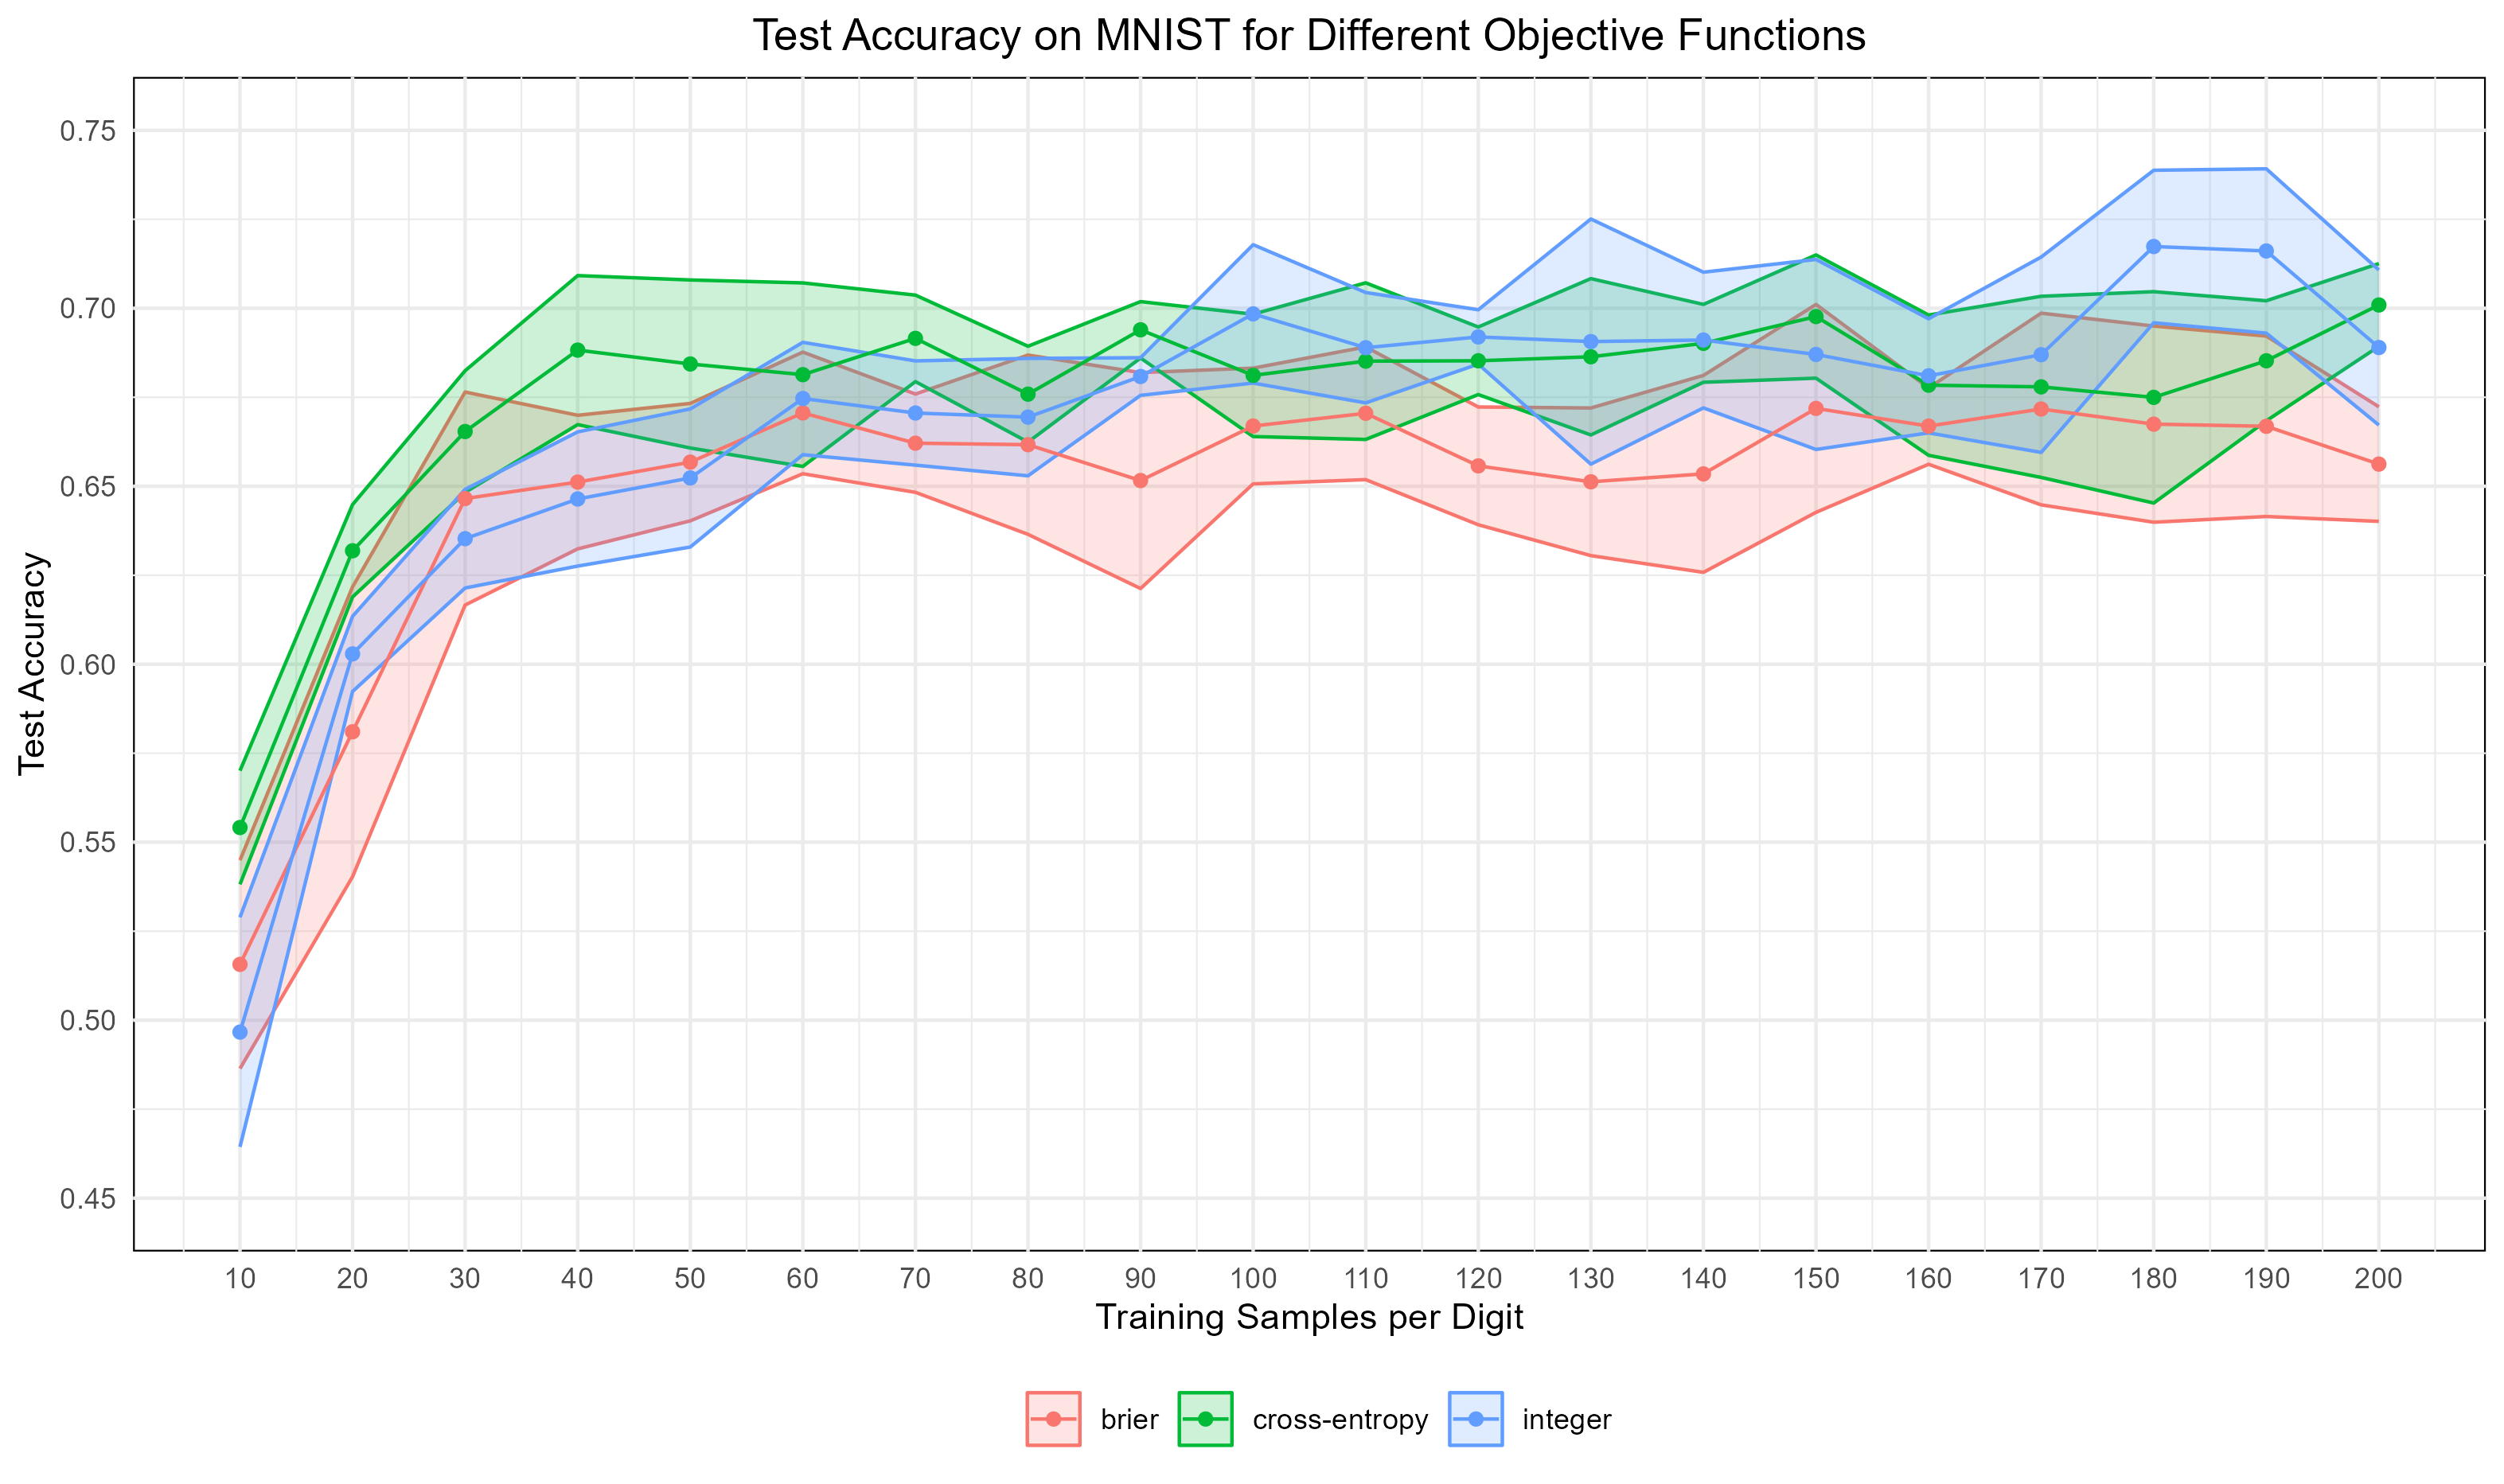
\includegraphics[width=1\linewidth]{Figures/SBT_COF.png}
    \caption{\small{\textbf{Testing accuracies for training a single batch on an increasing number of training samples. The x-axis shows the number of samples from each class in the batch, and the y-axis shows the test accuracy. The results are for a BNN with a single hidden layer with 16 neurons using ILS with a time limit of 60 seconds. The batches are balanced, meaning that there are the same number of samples present from all classes. The testing accuracy is reported for 8000 samples, 800 from each class. The figure shows the mean accuracy of 5 runs as a line and the standard deviation of the accuracy as a shaded area around it.}} }
    \label{SBT_COF}
\end{figure}

\noindent This network architecture is also tested by \cite{thorbjarnason2023}, who only use a training set of 100 samples, 10 from each digit. Their best-performing model achieves an average testing accuracy of 51.1 \% with an average runtime of 1852 seconds. With the cross-entropy objective function, I achieve a mean testing accuracy of 55.41 \% for the same amount of data, but with a time limit of only 60 seconds. For the integer objective function, the result is a testing accuracy of 49.66 \%. Both of my results may very well be subject to improvement if the time limit is increased. Additionally, my results are based on a pure BNN, whereas their results are based on a TNN. My results also indicate that the network architecture, even though it is quite small, can find a model that generalizes better if the amount of training data increases. 



\subsubsection{Testing the Effect of the Time Limit}
As a next step, I investigate the effect of the time limit. Since the previous experiment showed that more training data give better results, there were signs that the effect tapers off as the amount of training data increased. The goal of this experiment is to investigate whether the results can improve if the training is given more time. I test with a batch size of 2000, but now with different time limits ranging from 1 minute to 5 minutes. The mean accuracies can be seen in Table \ref{SBT_TETL}, where it is evident that a time limit of 60 seconds was not enough. For all the objective functions, the accuracy increases as the time limit increases. The Brier objective function still cannot compete with the two other objective functions, which achieve very similar results. The maximum mean accuracy for this experiment is now 74.23 \%, a significant improvement from the 71.73\% obtained before.   

\begin{center}
% latex table generated in R 4.2.2 by xtable 1.8-4 package
% Sun Jun  2 20:23:13 2024
\begin{table}[!tb]
\centering
\begin{tabular}{|c|c|c|c|c|c|}
  \hline
ObjectiveFunction & TL: 60 & TL: 120 & TL: 180 & TL: 240 & TL: 300 \\ 
  \hline
brier & 0.6562 & 0.6896 & 0.7063 & 0.7113 & 0.7149 \\ 
   \hline
cross-entropy & 0.7009 & 0.7202 & 0.7298 & 0.7360 & 0.7423 \\ 
   \hline
integer & 0.6890 & 0.7150 & 0.7340 & 0.7407 & 0.7413 \\ 
   \hline
\end{tabular}
\caption{\small{\textbf{The mean test accuracies on MNIST for different time limits. The results are obtained by training a 
            BNN on a single batch with 200 samples for each digit. The algorithm used is the ILS algorithm
            with the perturbation size set to 25. The time limit is in seconds.}}} 
\label{SBT_TETL}
\end{table}

\end{center}


\subsubsection{Comparing Different Network Structures}
I also want to test the effect of the network architecture on the results. From the previous experiments, I found that increasing time limits and increasing amounts of data give better results. For this reason, I use a time limit of 300 seconds and again a total batch size of 2000 balanced sampled samples. Apart from the already tested network architecture with one layer with 16 neurons, I also try one with two layers, each with 16 neurons. I also try two larger networks with 128 neurons in each layer, where I test with one and two layers again. \\

\noindent From Table \ref{SBT_DNS}, it can be seen that the general pattern is that more neurons in the layers boost the accuracy significantly. For some reason, this does not seem to apply to the Brier objective function, where the accuracy decreases significantly. In deep learning, it often helps to add more layers, which is not the case here. The most likely reason for this is the fact that the amount of training data does not justify the second layer. This will be tested further in the next section. The cross-entropy objective function performs slightly better than the integer objective function in networks with only one hidden layer, but for networks with two hidden layers, the integer objective function outperforms the others. 

\begin{center}
% latex table generated in R 4.2.2 by xtable 1.8-4 package
% Sun May 26 21:59:08 2024
\begin{table}[H]
\centering
\begin{tabular}{|c|c|c|c|}
  \hline
Objective function & Hidden layers & 16 & 128 \\ 
  \hline
brier & One & 0.7149 & 0.5096 \\ 
   \hline
cross-entropy & One & 0.7423 & 0.8185 \\ 
   \hline
integer & One & 0.7413 & 0.8003 \\ 
   \hline
brier & Two & 0.5125 & 0.3795 \\ 
   \hline
cross-entropy & Two & 0.4844 & 0.6614 \\ 
   \hline
integer & Two & 0.5340 & 0.7284 \\ 
   \hline
\end{tabular}
\caption{The mean test accuracies on MNIST for different network structures. The results are obtained by training a BNN
            on a single batch with 2000 samples using the ILS algorithm with a time limit of 300 seconds.
            The columns indicates the width of the hidden layers} 
\label{SBT_DNS}
\end{table}

\end{center}



\subsubsection{Fine Tuning the Perturbation Size}

\noindent So far, I have used a fixed value for the number of weights to change values for in the perturbation phase. The goal of this experiment is to see if there is room for improvement, i.e. if changing the perturbation size changes the results for the better. Ideally, all the results should be re-run with a different perturbation size to see if any of the conclusions drawn so far change, but since each experiment takes a long time to run, this is not computationally feasible. Instead, I take the configurations from the best results obtained so far, and use them to test if changing the perturbation size improves the results further. The best result obtained so far was with the cross-entropy objective function and with a single hidden layer with 128 neurons. Since this is a relatively big network compared to some of the others, I also test changing the perturbation size for the network with 16 neurons in the hidden layer. The time limit is again 300 seconds. Besides 25, I now try with perturbation sizes of 5, 10, 15, 20, 30, 35 and 40 as well. \\

\noindent The results are given in Table \ref{SBT_FTPS}. For the small network architecture, the highest mean accuracy is achieved with a perturbation size of 40, whereas for the large network architecture it is with a perturbation size of 30. In general, the results show that the perturbation size should not be too small. This is likely because small perturbation sizes might mean that the solution returns to the same local optima. This hyperparameter experiment also shows that for the small network architecture tested in the first experiments, it is possible to achieve an even better accuracy of 75.95\%, again with only 2000 data samples. Furthermore, with a larger network, it is possible to achieve as high an accuracy as 82.20\% using only this limited amount of data. 

\begin{center}
% latex table generated in R 4.2.2 by xtable 1.8-4 package
% Sun May 26 21:59:12 2024
\begin{table}[H]
\centering
\begin{tabular}{|c|c|c|c|}
  \hline
NeuronsHiddenLayer & PerturbationSize & Mean & SD \\ 
  \hline
16 &     5 & 0.7050 & 0.0085 \\ 
   \hline
16 &    10 & 0.7127 & 0.0153 \\ 
   \hline
16 &    15 & 0.7272 & 0.0240 \\ 
   \hline
16 &    20 & 0.7384 & 0.0207 \\ 
   \hline
16 &    25 & 0.7423 & 0.0074 \\ 
   \hline
16 &    30 & 0.7575 & 0.0129 \\ 
   \hline
16 &    35 & 0.7504 & 0.0149 \\ 
   \hline
16 &    40 & 0.7595 & 0.0153 \\ 
   \hline
128 &     5 & 0.8135 & 0.0041 \\ 
   \hline
128 &    10 & 0.8159 & 0.0018 \\ 
   \hline
128 &    15 & 0.8179 & 0.0042 \\ 
   \hline
128 &    20 & 0.8154 & 0.0037 \\ 
   \hline
128 &    25 & 0.8185 & 0.0058 \\ 
   \hline
128 &    30 & 0.8220 & 0.0054 \\ 
   \hline
128 &    35 & 0.8204 & 0.0040 \\ 
   \hline
128 &    40 & 0.8209 & 0.0076 \\ 
   \hline
\end{tabular}
\caption{The mean test accuracies on MNIST for two different networks with a single hidden layer.
            The results are obtained by training a BNN on a single batch with 2000 samples using the ILS
            algorithm with a time limit of 300 seconds. } 
\label{SBT_FTPS}
\end{table}

\end{center}


\subsection{Multiple Batch Training}
The goal of this section is to go a step further and train on more data using multiple batch training. The main motivation is that seeing more training data should help the model generalize better, but the important question is how to make use of more training data. From the first section, it was already clear that using more data in a single batch setting requires more time. Instead of trying to continue to increase the batch size and train on a single batch, I want to train a model that sees many batches throughout the training. In this section, I work with an overall time limit of 600 seconds.\\

\noindent There are three algorithms that I test and compare against each other. I test two versions of Algorithm \ref{multiple_batches}, the first version is as the algorithm is presented with iterated improvement for each batch. The other version is with iterated local search for each batch. The goal of this experiment is to investigate whether it helps to see more data, but for less time, which is the case for the iterated improvement version, or if it is better to see less data, but find a better solution each time. These algorithms use early stopping to make sure that the solution returned is not too dependent on the last batch seen. The third algorithm is Algorithm \ref{multiple_batches_v2}, where fewer moves are committed, but every move should generalize better, as a move is only committed if it improves the solution across several batches. The main question is whether this algorithm can compete against the others and whether it is too slow compared to the others. \\

\noindent In this section, I do not use balanced training and test sets anymore. MNIST is not uniformly distributed, and the main reason for using balanced training and test set was to make fair comparisons against existing literature. I still train on a BNN, and I use a batch size of 1,000. Whenever I use early stopping, I take 20 \% of the training set, 12,000 samples, and use it as a validation set. For iterated improvement I calculate the validation accuracy after every fourth batch, whereas for ILS I do it after every single batch. I test the same four network architectures as earlier. The accuracies are calculated on the full test set of 10,000 samples. \\

\noindent The first experiment in this section is again to test objective functions against each other and to see if they perform differently under different circumstances. For this, I test the three different objective functions on four different network structures and with all three algorithms. Afterwards I investigate whether the sporadic local search has any positive impact by testing the $bp$ parameter. 

\subsubsection{Comparing Objective Functions}
The goal of the first experiment is to see what objective function and algorithm work best. I use the settings specified above. For the ILS version, I let each ILS phase take 5 seconds and set $ps=25$. For all the algorithms, I set $bp=0.2$. I set $updateStart=1$, $updateEnd=15$ and $updateIncrease=10$. Table \ref{MBT} presents the mean accuracies. For the networks with 16 neurons in each hidden layer, it is the case for all configurations that the single layer version performs best. Furthermore, for the network with 16 neurons and a single hidden layer, the Brier objective function now performs almost as well as the cross-entropy in two of the algorithms and for the aggregation algorithm, it performs even slightly better. With two hidden layers, each with 16 neurons, the Brier score objective function clearly outperforms the other objective functions. \\

\begin{center}
% latex table generated in R 4.2.2 by xtable 1.8-4 package
% Sat May 25 12:43:53 2024
\begin{table}[H]
\centering
\begin{tabular}{|c|c|c|c|c|}
  \hline
Objective function & Hidden layers & Algorithm & 16 & 128 \\ 
  \hline
brier & One & Iterated Improvement & 0.8205 & 0.8479 \\ 
   \hline
brier & One & Aggregation Algorithm & 0.8491 & 0.8858 \\ 
   \hline
brier & One & Iterated Local Search & 0.7938 & 0.8499 \\ 
   \hline
cross-entropy & One & Iterated Improvement & 0.8223 & 0.8432 \\ 
   \hline
cross-entropy & One & Aggregation Algorithm & 0.8478 & 0.8655 \\ 
   \hline
cross-entropy & One & Iterated Local Search & 0.7992 & 0.8416 \\ 
   \hline
integer & One & Iterated Improvement & 0.8038 & 0.8668 \\ 
   \hline
integer & One & Aggregation Algorithm & 0.7919 & 0.8781 \\ 
   \hline
integer & One & Iterated Local Search & 0.7887 & 0.8632 \\ 
   \hline
brier & Two & Iterated Improvement & 0.7852 & 0.7005 \\ 
   \hline
brier & Two & Aggregation Algorithm & 0.8265 & 0.8454 \\ 
   \hline
brier & Two & Iterated Local Search & 0.7458 & 0.7191 \\ 
   \hline
cross-entropy & Two & Iterated Improvement & 0.7390 & 0.6736 \\ 
   \hline
cross-entropy & Two & Aggregation Algorithm & 0.6936 & 0.7997 \\ 
   \hline
cross-entropy & Two & Iterated Local Search & 0.7048 & 0.6986 \\ 
   \hline
integer & Two & Iterated Improvement & 0.5677 & 0.8878 \\ 
   \hline
integer & Two & Aggregation Algorithm & 0.4416 & 0.9153 \\ 
   \hline
integer & Two & Iterated Local Search & 0.7095 & 0.8766 \\ 
   \hline
\end{tabular}
\caption{The mean test accuracies on MNIST for different network structures and algorithms. The network is a
            BNN trained with a time limit of 600 seconds. Iterated Improvement and Iterated Local Search refers to
            Algorithm 4, and here early stopping is used. The validation dataset is 12,000 samples and for
            II, the validation accuracy is calculated every fourth batch, whereas for ILS, it is after every batch.
            The solution with the highest validation accuracy is returned. I set bp equal to 0.2 and ps to 25.
            Each ILS phase is allowed to run for 5 seconds. 
            For the Aggregation Algorithm, I do not use early stopping, but return the solution at the end. The parameters
            updateStart, updateEnd and updateIncrease are set to 1, 15 and 10 respectively. For all the algorithms
            a batch size of 1000 is used. } 
\label{MBT}
\end{table}

\end{center}


\noindent When the network size increases, the results are different. For both networks with a single hidden layer and two hidden layers, each with 128 neurons, the aggregation algorithm is the best. What is more surprising is that the integer objective function is now the best in all cases except for the one layer case with the aggregation algorithm. With two hidden layers, the integer objective function clearly outperforms the other objective functions. One of the reasons why this objective function is better might be due to the fact that it is much faster. To see this, look at Table \ref{MBT_II}, where I take a deeper look into the iterated improvement version of Algorithm \ref{multiple_batches}. Specifically, I take a look at how many batches the different objective functions iterate through within the time limit of 600 seconds. Here, it is clear, that for all the configurations, the integer objective function iterates through more batches and as a result sees more data. \\

\begin{center}
% latex table generated in R 4.2.2 by xtable 1.8-4 package
% Sun Jun  2 21:10:30 2024
\begin{table}[!tb]
\centering
\begin{tabular}{|c|c|c|c|c|c|}
  \hline
Objective function & Hidden layers & Mean & MeanBatches & MeanMoves & MeanMoves30 \\ 
  \hline
brier & 16 & 0.8205 & 427.20 & 213.0588 & 236.5333 \\ 
   \hline
cross-entropy & 16 & 0.8223 & 475.20 & 174.5439 & 217.9800 \\ 
   \hline
integer & 16 & 0.8038 & 594.20 & 107.2392 & 115.9400 \\ 
   \hline
brier & 16-16 & 0.7852 & 392.80 & 179.3991 & 181.5333 \\ 
   \hline
cross-entropy & 16-16 & 0.7390 & 394.60 & 183.8709 & 178.2067 \\ 
   \hline
integer & 16-16 & 0.5677 & 591.60 & 66.0823 & 84.8200 \\ 
   \hline
brier & 128 & 0.8479 & 45.80 & 4205.4210 & 4191.3800 \\ 
   \hline
cross-entropy & 128 & 0.8432 & 62.60 & 2854.2981 & 2988.1267 \\ 
   \hline
integer & 128 & 0.8668 & 147.80 & 993.4502 & 1158.5133 \\ 
   \hline
brier & 128-128 & 0.7005 & 48.40 & 2542.8706 & 2049.0067 \\ 
   \hline
cross-entropy & 128-128 & 0.6736 & 47.00 & 2579.0009 & 2537.3467 \\ 
   \hline
integer & 128-128 & 0.8878 & 110.80 & 887.7500 & 935.8800 \\ 
   \hline
\end{tabular}
\caption{\small{\textbf{Summary statistics for the iterated improvement version of Algorithm 4. 
            'MeanBatches' is the average number of batches seen, MeanMoves' is the average number of moves made per batch,
            and MeanMoves30 is the average number of moves made per batch in the first 30 batches.}}} 
\label{MBT_II}
\end{table}

\end{center}


\noindent I also take a look at the number of moves made per batch. As this number is expected to decrease as the number of batches increases, I also present the number for the first 30 batches. In both cases, the pattern is the same. For the integer objective function, fewer moves are made. This suggests that the number of batches seen is not higher only because the integer objective function is faster in computation time, but also because fewer moves are made in each iteration. This is not necessarily a bad thing. The more moves that are made at each iteration, the more the current solution depends on the current batch. As a result, the gap between training accuracy and validation or test accuracy might be larger for the objective functions that make more moves based on the current batch. This is especially evident from Figure \ref{MBT_II_INTEGER}, \ref{MBT_II_BRIER} and \ref{MBT_II_CROSS_ENTROPY_FUNCTION} that plots the training accuracies and the validation accuracies for each of the three objective functions. The plots are based on the iterated improvement algorithm and a network architecture with two hidden layers with 128 neurons each. The gap is quite small for the integer objective function compared to the Brier and cross-entropy objective functions. \\

\noindent These are possible reasons why the integer objective function is better, but they do not necessarily explain why it is only better for larger networks. However, this is probably due to the definition of the integer objective function, which does not work with probability or probability distributions, but with maximizing the margins. For small networks, it seems that this is not possible in the same way as with larger networks, where the integer objective function is better than the other objective functions in most cases. 

\begin{figure}[H]
    \centering
    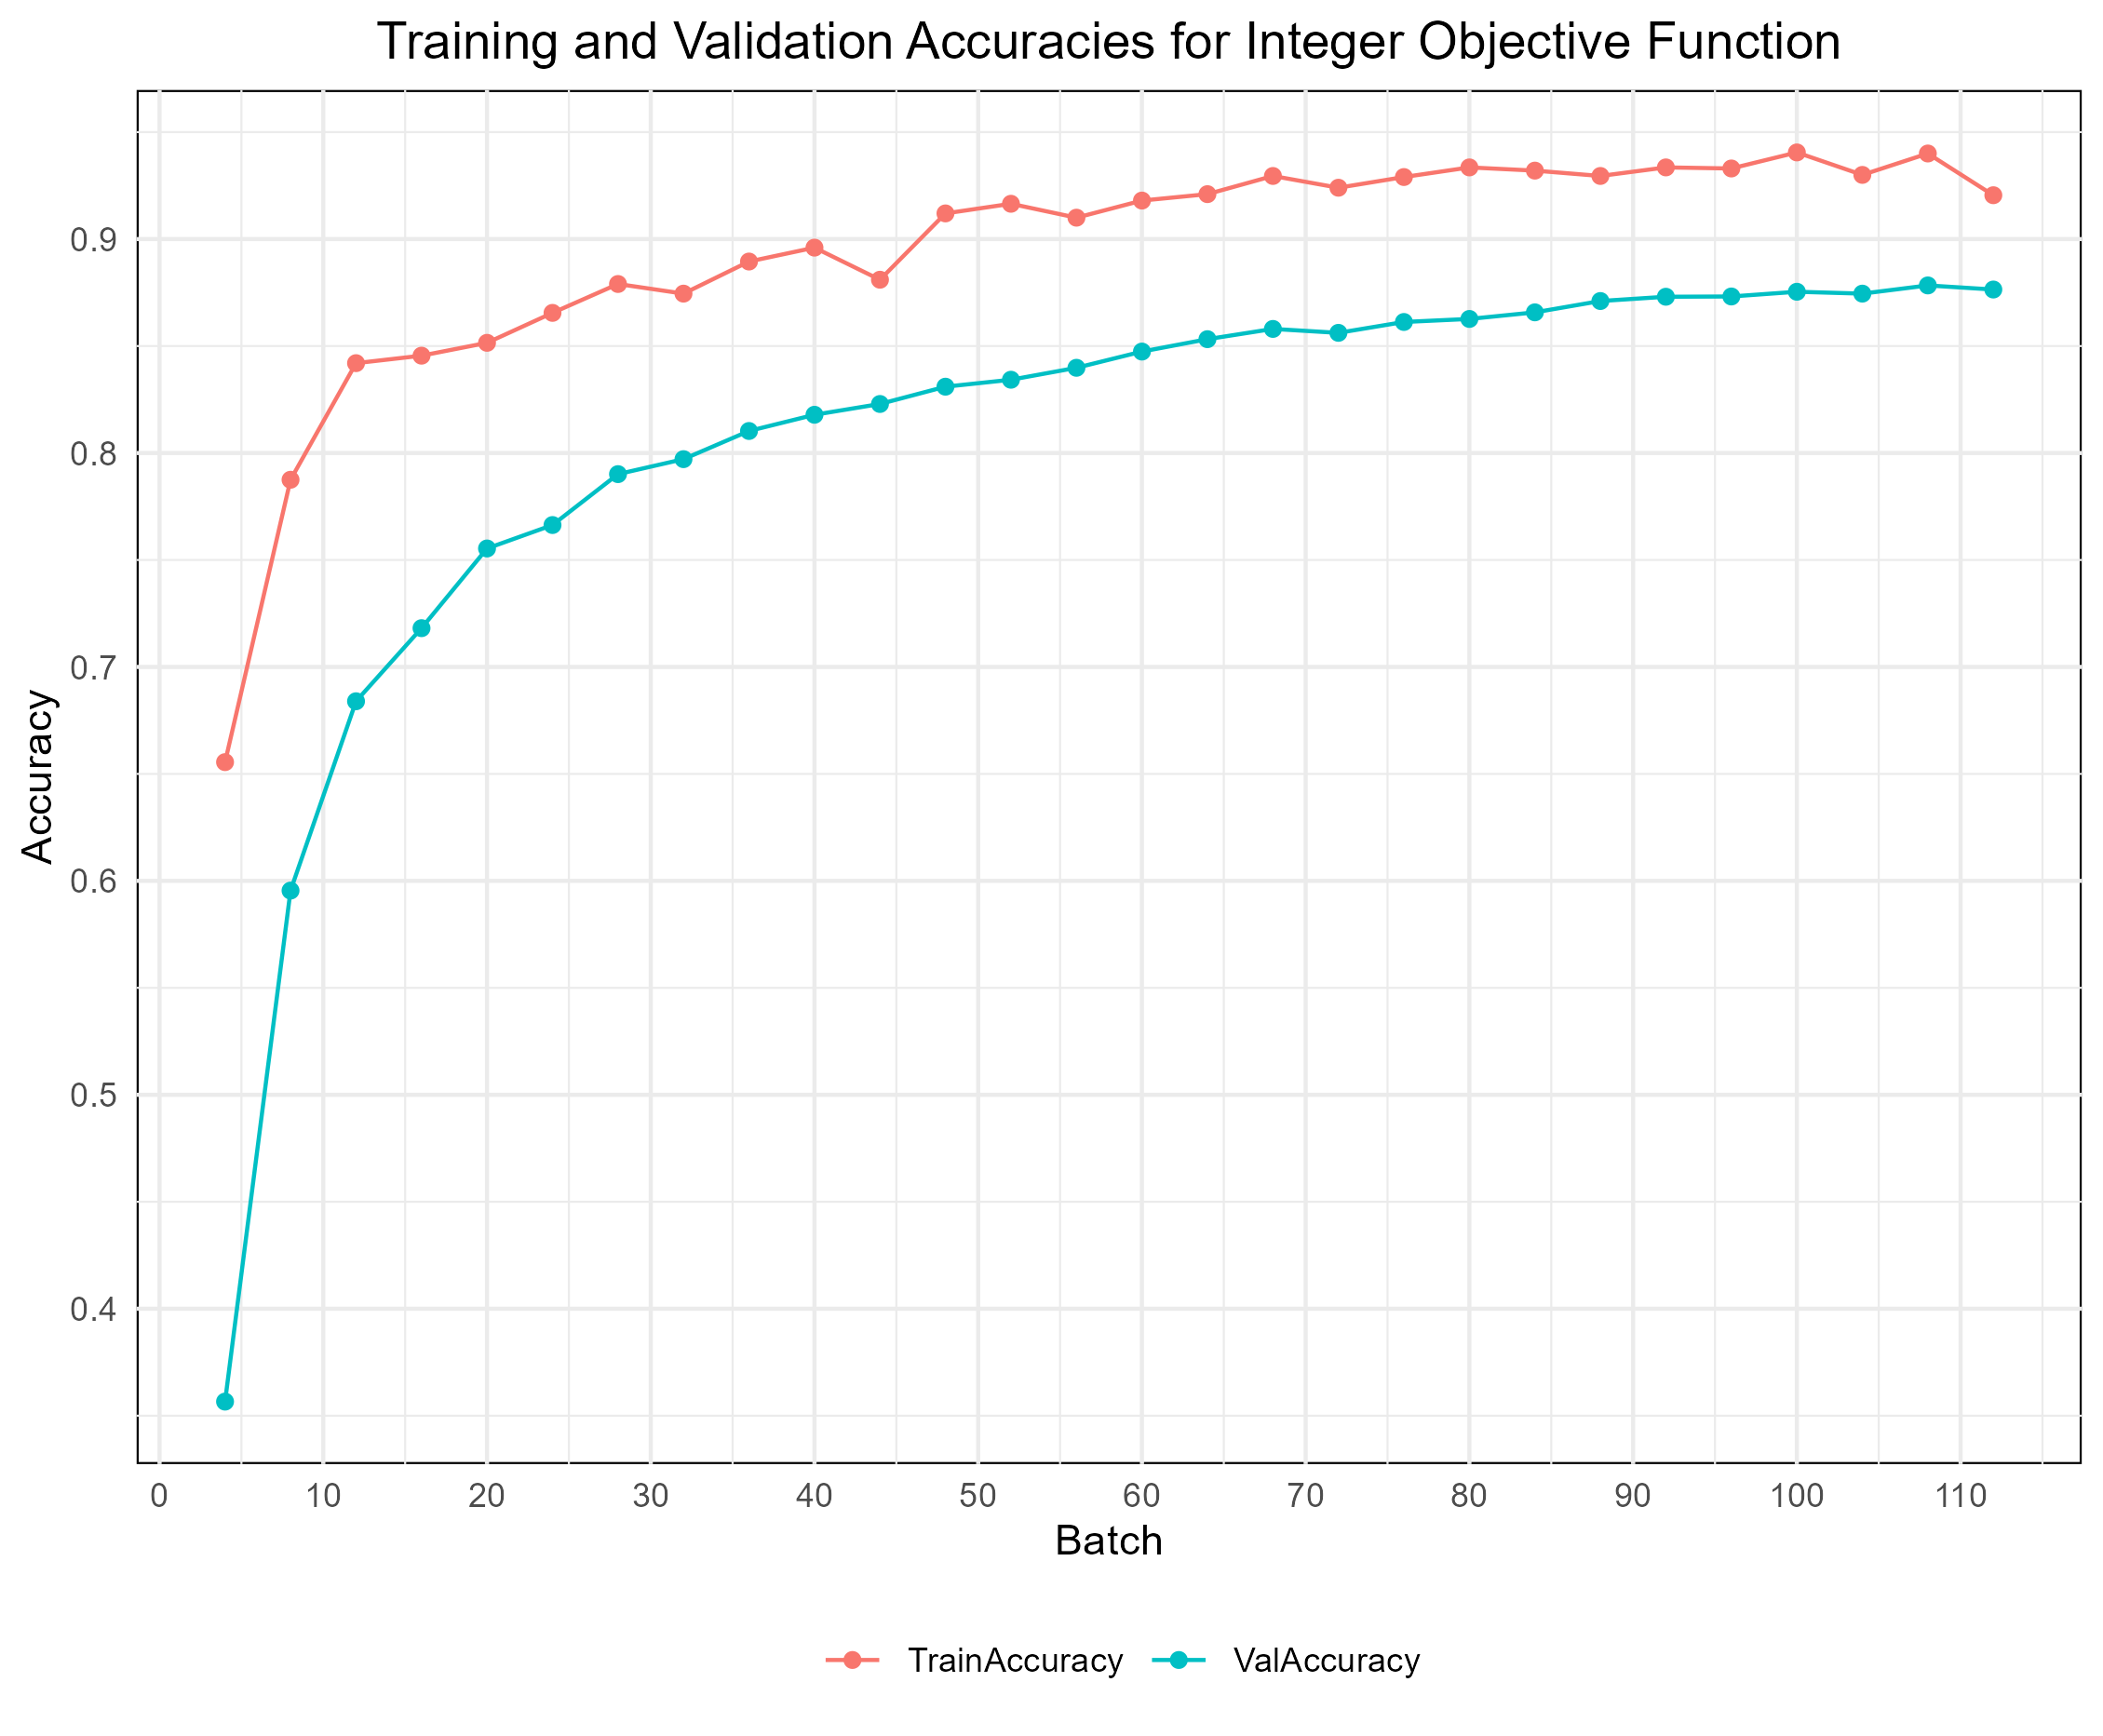
\includegraphics[width=1\linewidth]{Figures/MBT_II_INTEGER.png}
    \caption{\small{\textbf{Training and validation accuracies for the iterated improvement algorithm with the integer objective function. The network structure is with two hidden layers, each with 128 neurons in each. As such, the plot is for the last row of Table \ref{MBT_II}.}}}
    \label{MBT_II_INTEGER}
\end{figure}

\begin{figure}[H]
    \centering
    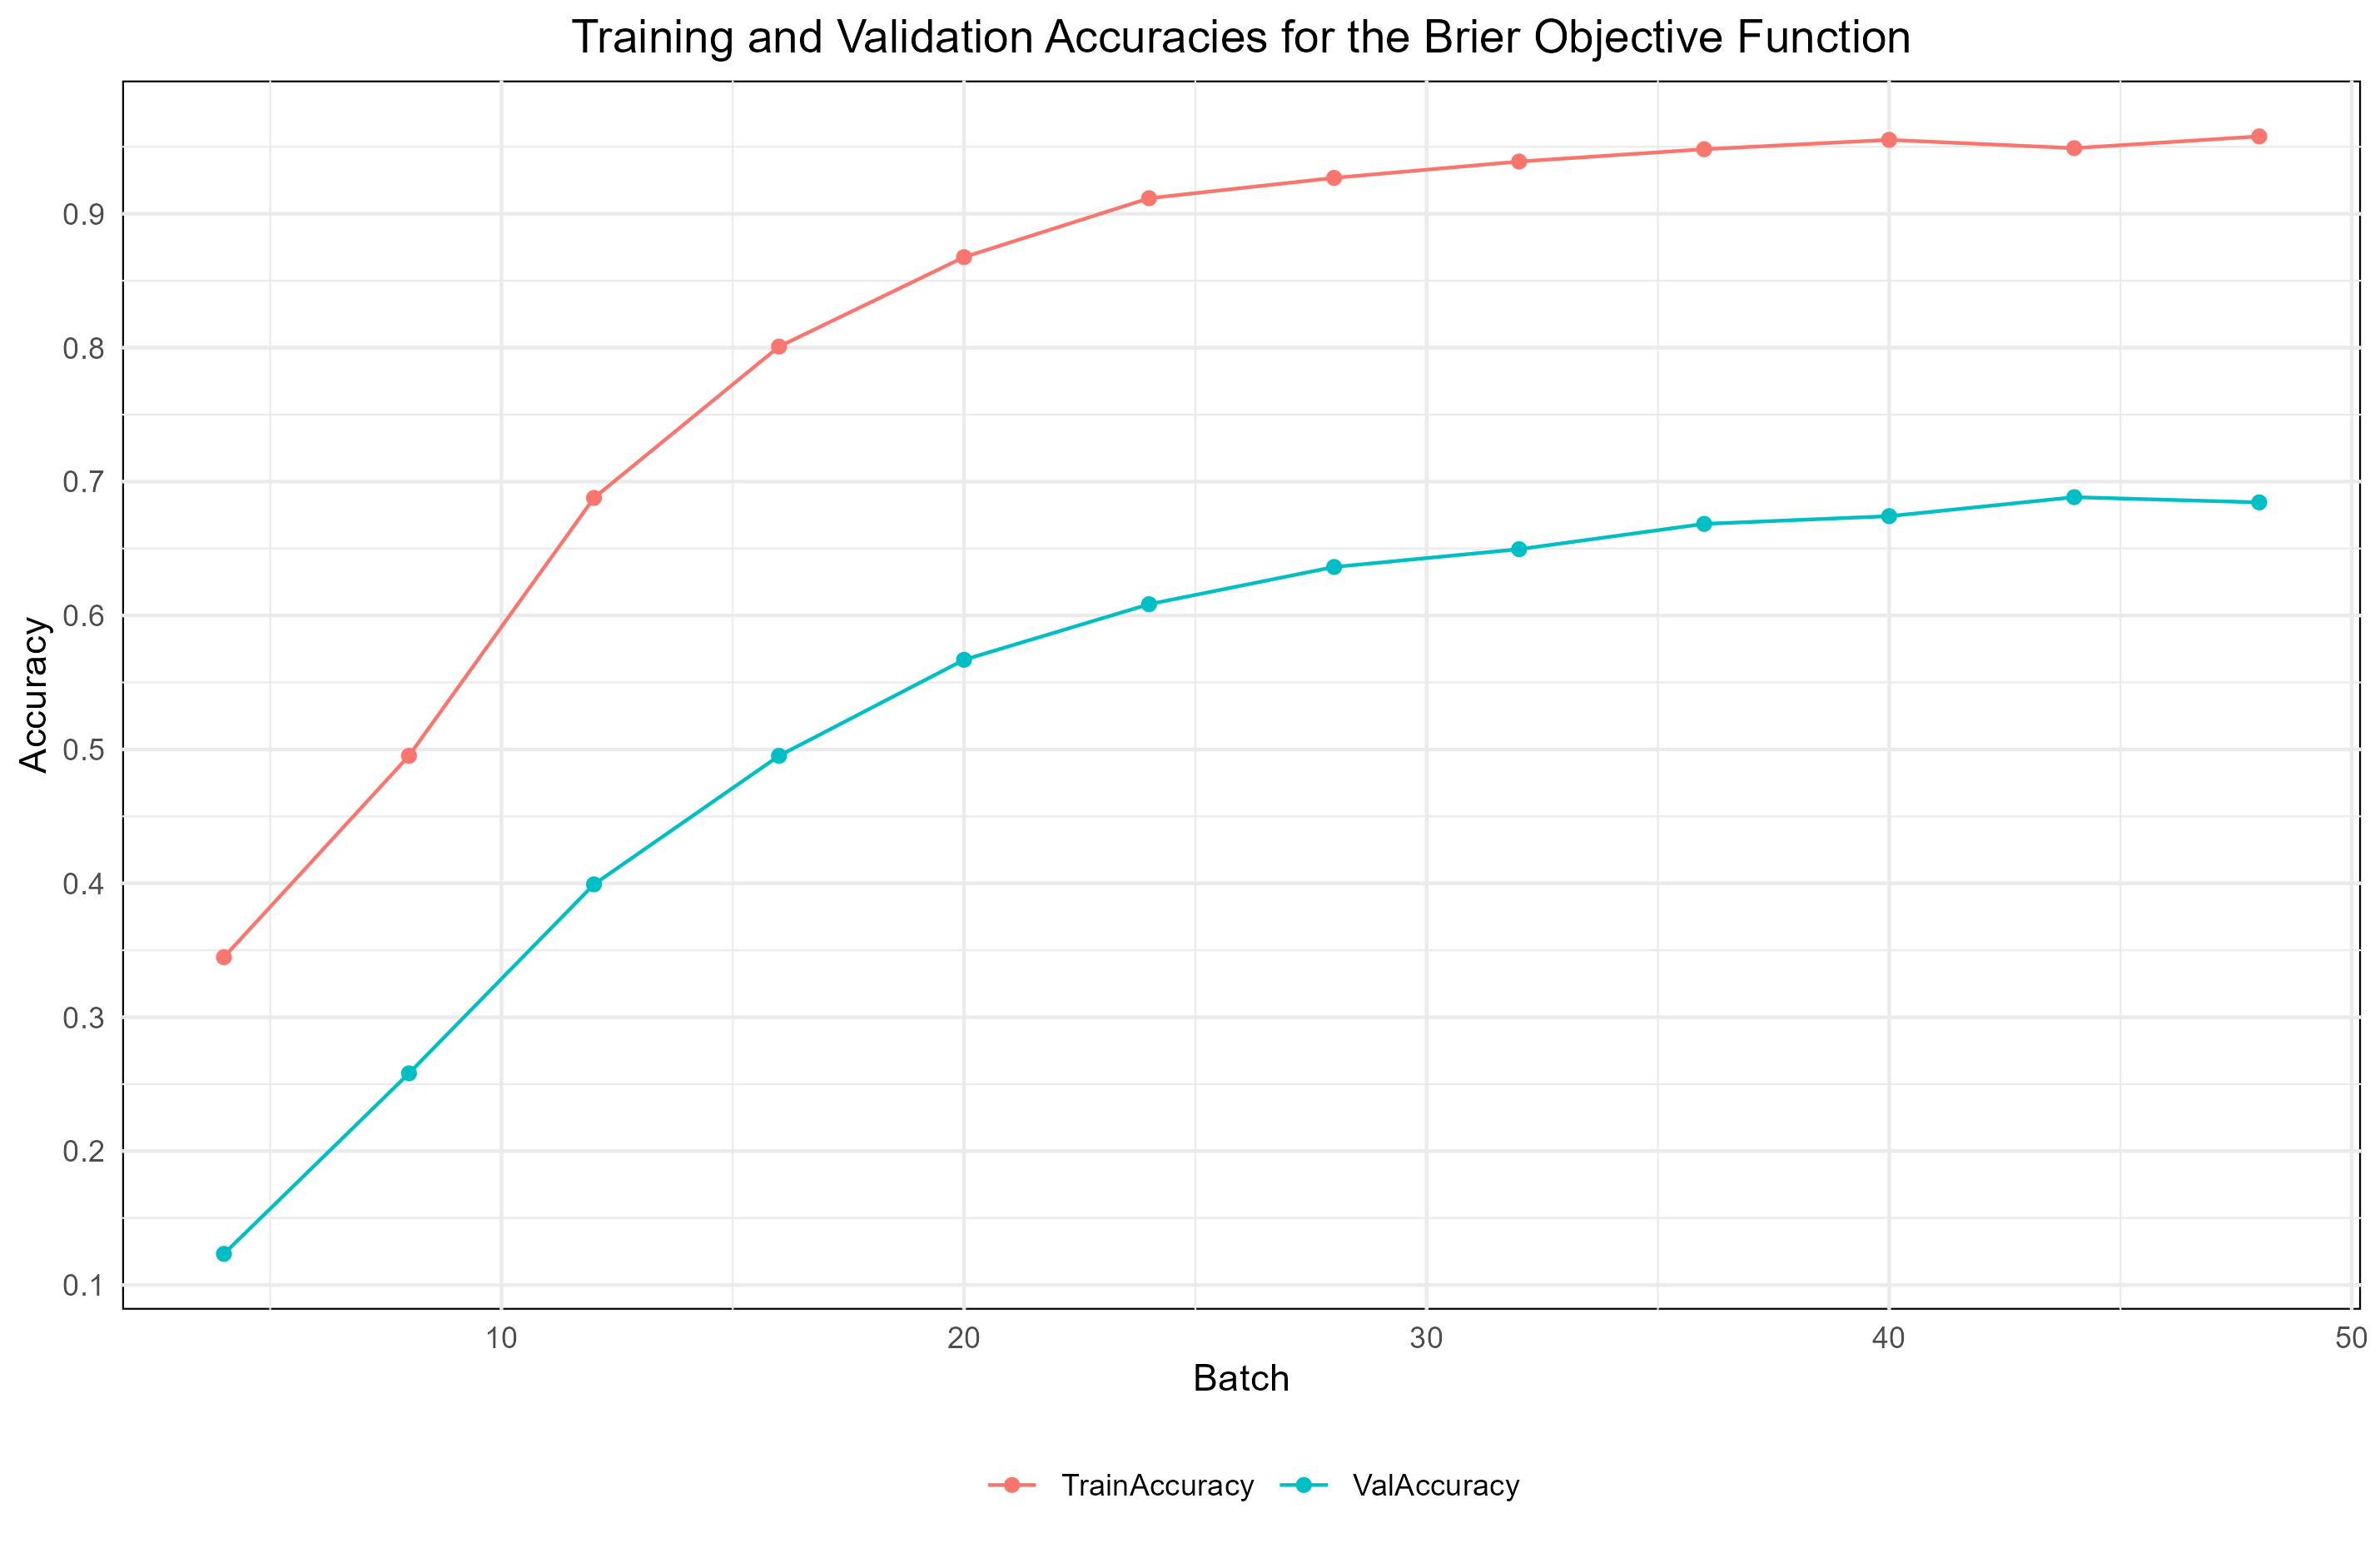
\includegraphics[width=1\linewidth]{Figures/MBT_II_BRIER.png}
    \caption{\small{\textbf{Training and validation accuracies for the iterated improvement algorithm with the Brier objective function. The network structure is with two hidden layers, each with 128 neurons in each. As such, the plot is for the third last row of Table \ref{MBT_II}.}}}
    \label{MBT_II_BRIER}
\end{figure}

\begin{figure}[H]
    \centering
    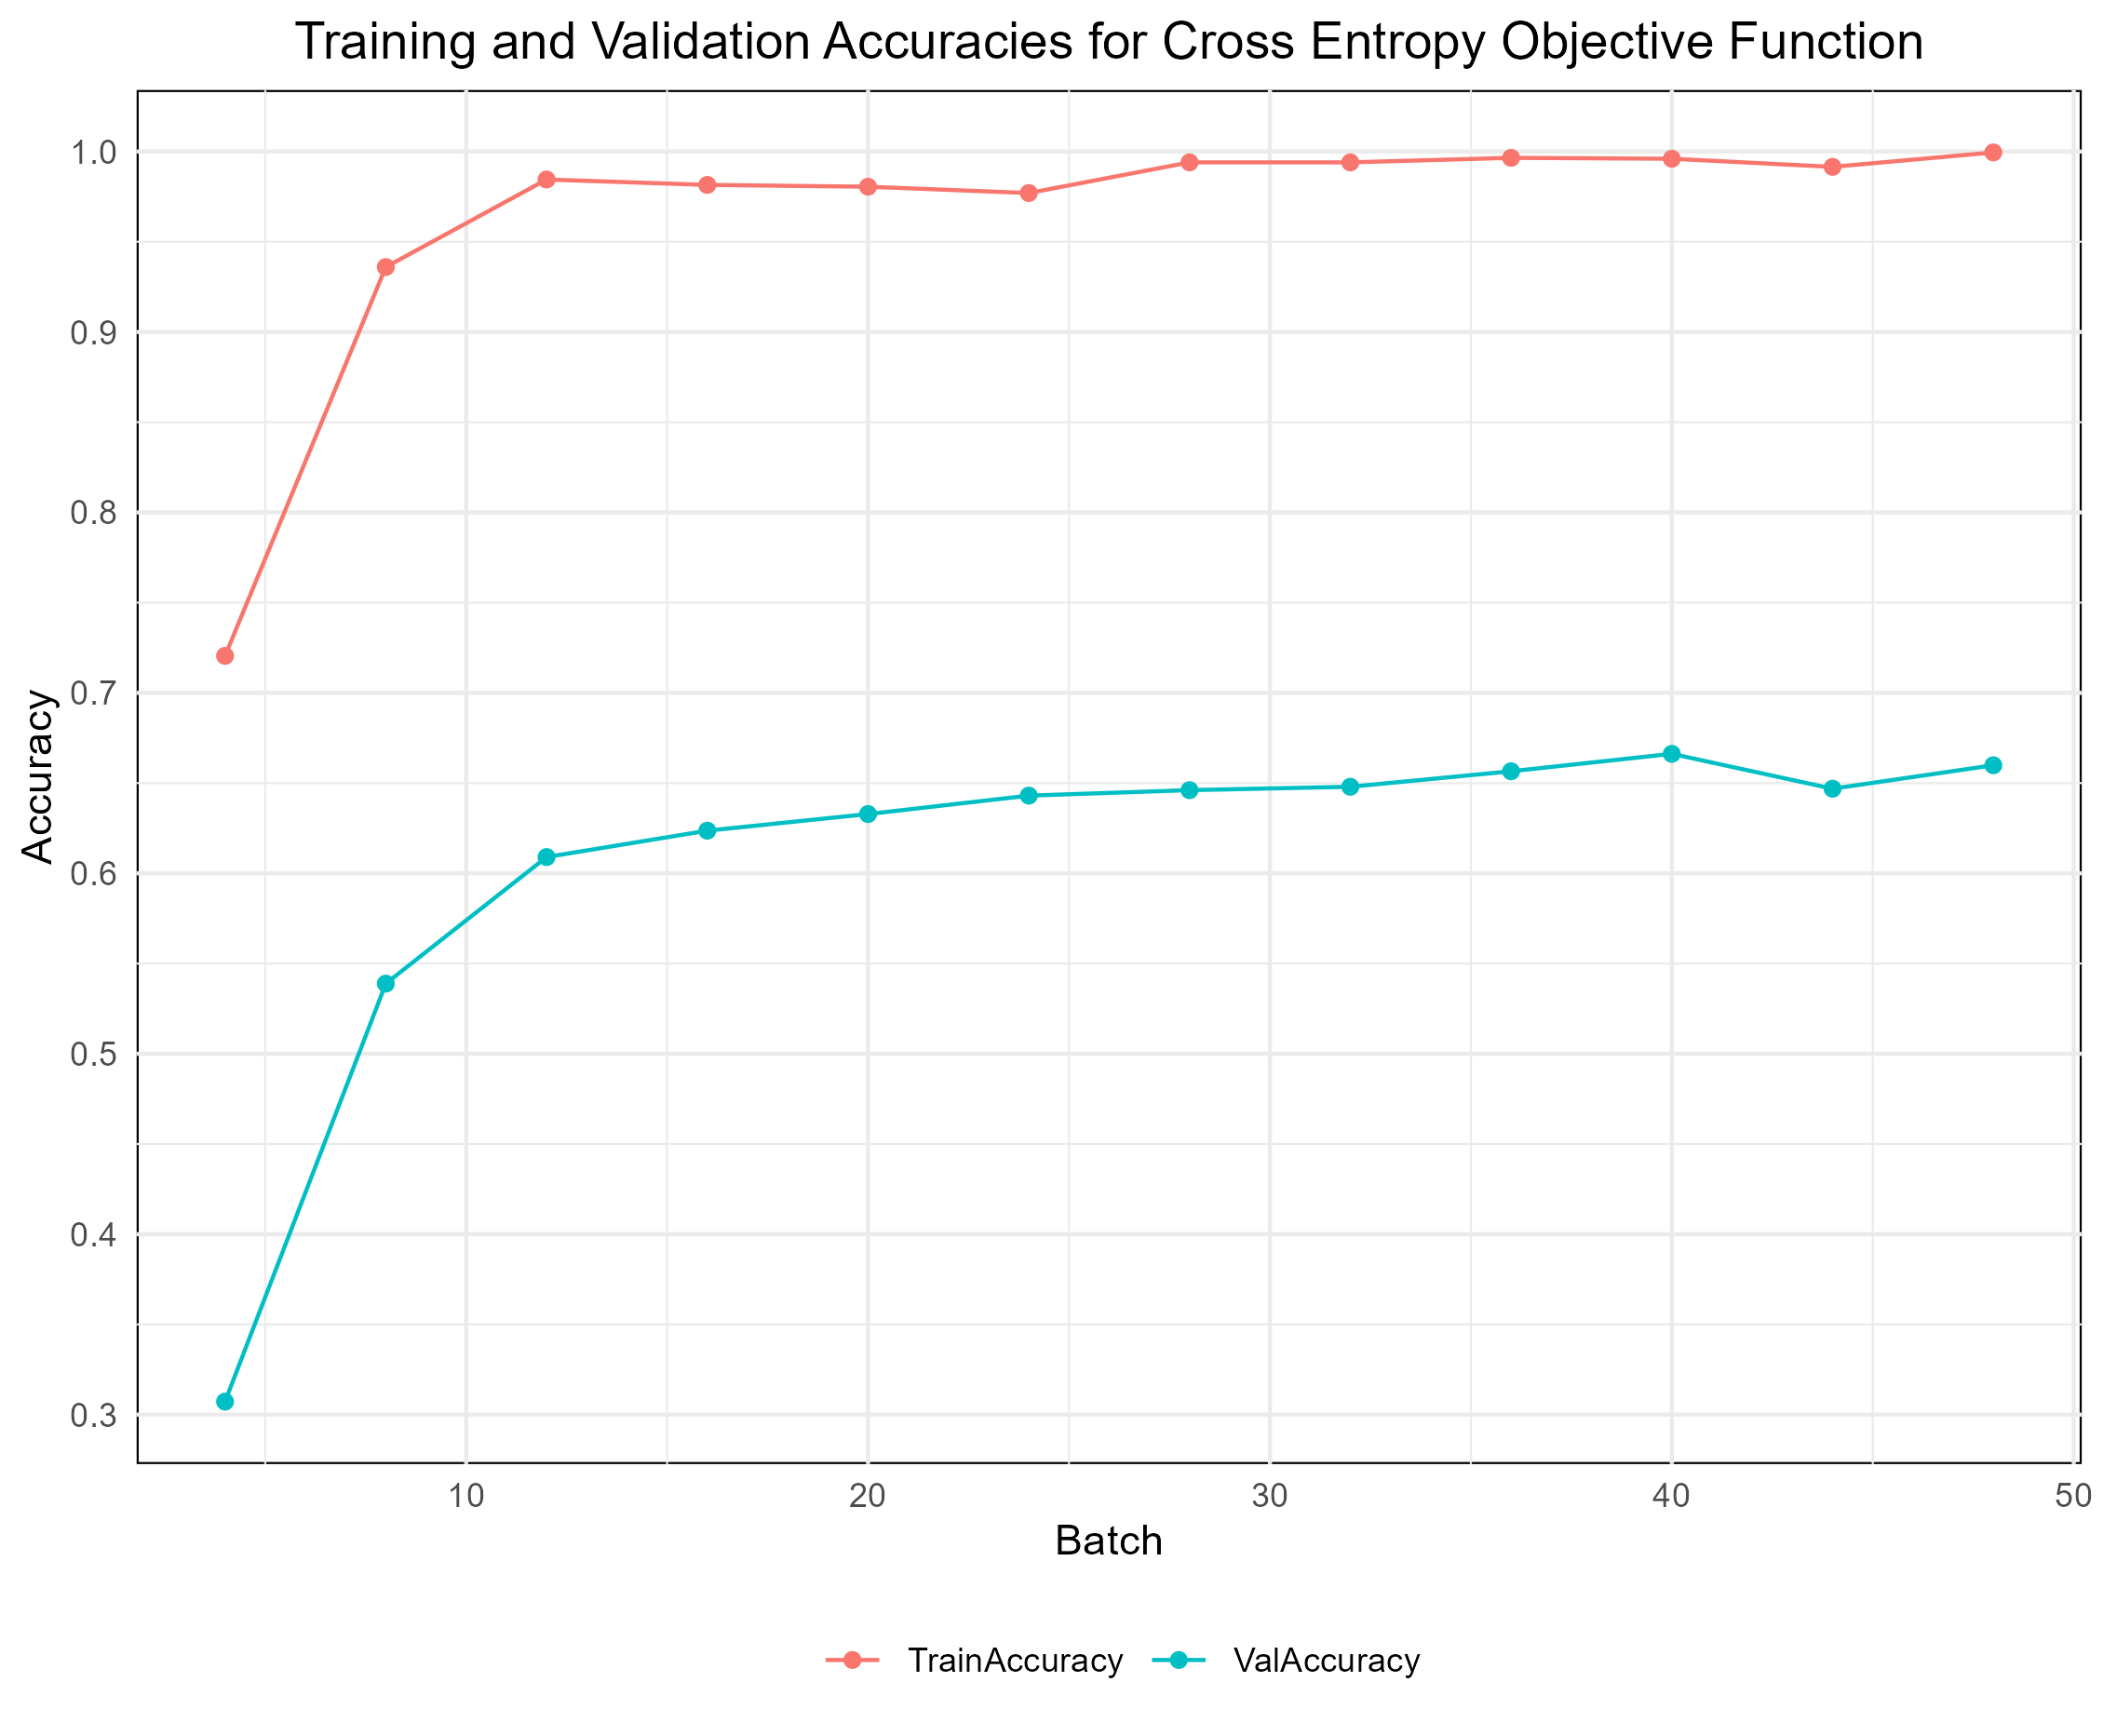
\includegraphics[width=1\linewidth]{Figures/MBT_II_CROSS_ENTROPY.png}
    \caption{\small{\textbf{Training and validation accuracies for the iterated improvement algorithm with the cross-entropy objective function. The network structure is with two hidden layers, each with 128 neurons in each. As such, the plot is for the second last row of Table \ref{MBT_II}.}}}
    \label{MBT_II_CROSS_ENTROPY_FUNCTION}
\end{figure}

\subsubsection{Testing the Effect of Sporadic Local Search}
For all three algorithms, I used sporadic local search, where the parameter $bp$ determines the probability that a weight is part of the search in that iteration. Until now, I used $bp=0.2$, but now I will change the value of this to see how important it is and if it has any effect at all. Note that $bp=1$ corresponds to not using sporadic local search, as in this case all weights are subject to change in each iteration. The hope is that using sporadic local search would improve the ability of the model to generalize by being less dependent on the current batch. For the aggregation algorithm, this is not necessarily true, as the algorithm does not make moves based on a single batch. Instead of $bp=0.2$, I will try with 0.1, 0.3, 0.4, 0.5, and 1 as values. I use the best configuration from the previous experiment, so I use a network architecture with 2 hidden layers, each with 128 neurons, and I use the integer objective function. \\
\noindent The mean test accuracies can be seen in Table \ref{MBT_FTBP}, where the results are somewhat disappointing. For ILS and iterated improvement, the test accuracies are better with no use of sporadic local search, and for the aggregation algorithm, the results are very similar across different values of $bp$, so there seems to be no positive effect of using sporadic local search. 


\begin{center}
% latex table generated in R 4.2.2 by xtable 1.8-4 package
% Sun Jun  2 21:27:35 2024
\begin{table}[!tb]
\centering
\begin{tabular}{|c|c|c|c|}
  \hline
Algorithm & BP & Mean & SD \\ 
  \hline
Iterated Improvement & 0.1 & 0.8825 & 0.0030 \\ 
   \hline
Iterated Improvement & 0.2 & 0.8878 & 0.0033 \\ 
   \hline
Iterated Improvement & 0.3 & 0.8917 & 0.0039 \\ 
   \hline
Iterated Improvement & 0.4 & 0.8896 & 0.0051 \\ 
   \hline
Iterated Improvement & 0.5 & 0.8917 & 0.0033 \\ 
   \hline
Iterated Improvement & 1.0 & 0.8976 & 0.0030 \\ 
   \hline
Aggregation Algorithm & 0.1 & 0.9130 & 0.0030 \\ 
   \hline
Aggregation Algorithm & 0.2 & 0.9153 & 0.0025 \\ 
   \hline
Aggregation Algorithm & 0.3 & 0.9125 & 0.0009 \\ 
   \hline
Aggregation Algorithm & 0.4 & 0.9132 & 0.0013 \\ 
   \hline
Aggregation Algorithm & 0.5 & 0.9131 & 0.0032 \\ 
   \hline
Aggregation Algorithm & 1.0 & 0.9147 & 0.0032 \\ 
   \hline
Iterated Local Search & 0.1 & 0.8564 & 0.0054 \\ 
   \hline
Iterated Local Search & 0.2 & 0.8766 & 0.0050 \\ 
   \hline
Iterated Local Search & 0.3 & 0.8806 & 0.0039 \\ 
   \hline
Iterated Local Search & 0.4 & 0.8826 & 0.0031 \\ 
   \hline
Iterated Local Search & 0.5 & 0.8844 & 0.0038 \\ 
   \hline
Iterated Local Search & 1.0 & 0.8939 & 0.0033 \\ 
   \hline
\end{tabular}
\caption{\small{\textbf{The mean test accuracies on MNIST for three different algorithms with different values of bp.
            The results are obtained by training a BNN for a time limit of 600 seconds. For II, k=4, for
            ILS, k=1 and each ILS phase runs for 5 seconds with a perturbation size of 25. For AA updateStart, updateEnd
            and updateIncrease are 1, 15 and 10 respectively.}}} 
\label{MBT_FTBP}
\end{table}

\end{center}



\subsection{Ternary Neural Networks}
\noindent In a TNN, the weights can also be zero, which increases the capacity of the model. As a result, the solution space becomes bigger and the delta evaluation takes more time. When considering a move in a BNN, there is only one other possible value. For a TNN, two other values need to be considered. For this reason, I expect that training a TNN takes a longer time, but the hope is that, as the model has a larger capacity, it will be able to give higher accuracies as well. The goal of this section is to explore TNNs. At first I will test the effect of adding a regularization parameter, as introduced in Section 5.3.5. Second, I will investigate if it takes longer to train a TNN compared to a BNN. The results in these sections are comparable to existing literature on training NNs using MIP, so here I again use balanced training and test sets and train on a single batch.

\begin{center}
% latex table generated in R 4.2.2 by xtable 1.8-4 package
% Sat Jun  1 15:52:08 2024
\begin{table}[!tb]
\centering
\begin{tabular}{|c|c|c|c|c|c|}
  \hline
Reg & ObjectiveFunc & Mean & SD & Connections & LocalOptimas \\ 
  \hline
 0.00000 & brier & 0.7264 & 0.0209 & 8813 &  98 \\ 
   \hline
 0.00001 & brier & 0.7057 & 0.0124 & 5053 &  59 \\ 
   \hline
 0.00010 & brier & 0.7100 & 0.0095 & 4928 &  60 \\ 
   \hline
 0.00100 & brier & 0.7143 & 0.0137 & 4785 &  68 \\ 
   \hline
 0.01000 & brier & 0.7025 & 0.0047 & 4447 &  82 \\ 
   \hline
 0.10000 & brier & 0.7088 & 0.0177 & 3776 & 106 \\ 
   \hline
 1.00000 & brier & 0.7492 & 0.0089 & 1348 & 116 \\ 
   \hline
10.00000 & brier & 0.6811 & 0.0202 &  393 &  62 \\ 
   \hline
 0.00000 & cross-entropy & 0.7471 & 0.0158 & 8774 & 117 \\ 
   \hline
 0.00001 & cross-entropy & 0.7270 & 0.0076 & 5011 &  69 \\ 
   \hline
 0.00010 & cross-entropy & 0.7283 & 0.0175 & 4984 &  69 \\ 
   \hline
 0.00100 & cross-entropy & 0.7251 & 0.0095 & 4923 &  74 \\ 
   \hline
 0.01000 & cross-entropy & 0.7242 & 0.0093 & 4743 &  78 \\ 
   \hline
 0.10000 & cross-entropy & 0.7346 & 0.0128 & 4093 & 105 \\ 
   \hline
 1.00000 & cross-entropy & 0.7446 & 0.0112 & 2349 & 130 \\ 
   \hline
10.00000 & cross-entropy & 0.7359 & 0.0123 &  228 &  65 \\ 
   \hline
 0.00000 & integer & 0.7315 & 0.0174 & 8690 & 235 \\ 
   \hline
 0.00001 & integer & 0.7120 & 0.0143 & 4462 & 130 \\ 
   \hline
 0.00010 & integer & 0.7134 & 0.0139 & 4461 & 131 \\ 
   \hline
 0.00100 & integer & 0.7121 & 0.0142 & 4462 & 130 \\ 
   \hline
 0.01000 & integer & 0.7127 & 0.0139 & 4462 & 130 \\ 
   \hline
 0.10000 & integer & 0.7140 & 0.0138 & 4462 & 131 \\ 
   \hline
 1.00000 & integer & 0.7214 & 0.0153 & 4166 & 127 \\ 
   \hline
10.00000 & integer & 0.7257 & 0.0196 & 1212 & 142 \\ 
   \hline
\end{tabular}
\caption{\small{\textbf{Summary statistics for single batch training of a TNN with 2000 samples. 
          The network trained has a single hidden layer with 16 neurons and is trained for
          300 seconds.}}} 
\label{TNN_COF}
\end{table}

\end{center}


\subsubsection{Testing the Effect of a Regularization Parameter}
I start by testing the effect of the regularization parameter by testing different values. I train on a single batch, with 2000 samples, and the network has a single hidden layer with 16 neurons, so the most comparable results obtained so far are those from the Single Batch Training section. I test with all 3 objective functions and different values of the regularization parameter. Whenever this parameter is equal to zero, it corresponds to training a TNN without any additional regularization term. From Table \ref{SBT_TETL}, the results for training a BNN with the same settings are given. Here, for a time limit of 300 seconds, the accuracies were 71.49 \%, 74.23 \% and 74.13 \% for the Brier, cross-entropy and integer objective function respectively. From Table \ref{TNN_COF}, it can be seen that whenever no regularization parameter is added, the mean accuracies already increase for the Brier and cross-entropy objective functions, whereas for the integer objective function, the accuracy decreases compared to the BNN. \\

\noindent In Table \ref{TNN_COF}, the 'Connections' column shows the average number of active connections, i.e. the weights whose value is not 0. The same value of the regularization parameter does not seem to have the same effect across objective functions. It seems that the integer objective function needs higher values of the regularization parameter compared to the other objective functions. This is related to the definition of the objective function, and in particular the range of the objective function value. For the Brier objective function, there seems to be a positive effect of adding a regularization parameter of around 1.0, so I run another experiment to fine-tune this further. From Table \ref{TNN_REG_BRIER}, it seems to be the case that a value between 1.5 and 2.5 gives the highest accuracies with a maximum mean accuracy of 76.22 \% for a value of 2. For this value, the average number of active connections is 572. The total number of connections in the network is $784 \cdot 16 + 16 \cdot 10 = 12,704$, so it is less than 5\% of the connections that are actually active. \\



\noindent For the cross-entropy function, at first sight looking at Table \ref{TNN_COF}, there is no value of the regularization parameter that gives higher accuracy, but a value of 1.0 comes close, so again, I conduct another experiment to fine-tune further. Table \ref{TNN_REG_CS} shows that it was possible to find values of the regularization parameter that gave higher accuracies. The maximum mean accuracy here is 76.65 \%, but this time with a value of 4.0 for the regularization parameter. It is interesting to note that the average number of active connections in this case is 574, which is very close to the same number for the Brier objective function. For the integer objective function, there does not seem to be a positive effect, neither in Table \ref{TNN_COF} nor in \ref{TNN_REG_INT}, where I tested with more values. \\

\noindent It should be mentioned that this fine-tuning was with respect to the specific settings used here. By the way the objective function terms are defined, it is highly likely that changing either the number of connections in the network, i.e. the network architecture, or the number of samples in the batch, then a new fine-tuning is required. Thus, it is not expected that these values of the regularization parameter generalize well to other settings, but nevertheless, the results show that for the Brier and cross-entropy objective functions, there is something to be gained when regularizing the network. For the integer objective function, regularization did not seem to have any positive influence. 
\begin{center}
% latex table generated in R 4.2.2 by xtable 1.8-4 package
% Sat Jun  1 17:01:34 2024
\begin{table}[!tb]
\centering
\begin{tabular}{|c|c|c|c|c|c|}
  \hline
Reg & ObjectiveFunc & Mean & SD & Connections & LocalOptimas \\ 
  \hline
0.00 & brier & 0.7264 & 0.0209 & 8813 &  98 \\ 
   \hline
0.50 & brier & 0.7308 & 0.0099 & 2349 & 123 \\ 
   \hline
0.75 & brier & 0.7372 & 0.0116 & 1829 & 121 \\ 
   \hline
1.00 & brier & 0.7492 & 0.0089 & 1348 & 116 \\ 
   \hline
1.25 & brier & 0.7471 & 0.0036 & 1141 & 105 \\ 
   \hline
1.50 & brier & 0.7555 & 0.0078 &  844 &  95 \\ 
   \hline
1.75 & brier & 0.7545 & 0.0118 &  727 &  85 \\ 
   \hline
2.00 & brier & 0.7622 & 0.0136 &  572 &  85 \\ 
   \hline
2.25 & brier & 0.7511 & 0.0124 &  510 &  82 \\ 
   \hline
2.50 & brier & 0.7569 & 0.0098 &  441 &  79 \\ 
   \hline
2.75 & brier & 0.7467 & 0.0171 &  385 &  65 \\ 
   \hline
3.00 & brier & 0.7419 & 0.0111 &  365 &  62 \\ 
   \hline
3.25 & brier & 0.7435 & 0.0126 &  308 &  57 \\ 
   \hline
3.50 & brier & 0.7574 & 0.0087 &  265 &  57 \\ 
   \hline
3.75 & brier & 0.7489 & 0.0199 &  222 &  63 \\ 
   \hline
4.00 & brier & 0.7514 & 0.0121 &  221 &  61 \\ 
   \hline
\end{tabular}
\caption{\small{\textbf{Summary statistics for single batch training of a TNN with 2000 samples. 
          The network trained has a single hidden layer with 16 neurons and is trained for
          300 seconds.}}} 
\label{TNN_REG_BRIER}
\end{table}

\end{center}

\begin{center}
% latex table generated in R 4.2.2 by xtable 1.8-4 package
% Wed May 29 09:54:57 2024
\begin{table}[H]
\centering
\begin{tabular}{|c|c|c|c|c|c|}
  \hline
Reg & ObjectiveFunc & Mean & SD & Connections & LocalOptimas \\ 
  \hline
0.0 & cross-entropy & 0.7471 & 0.0158 & 8774 & 117 \\ 
   \hline
0.5 & cross-entropy & 0.7334 & 0.0098 & 3069 & 131 \\ 
   \hline
1.0 & cross-entropy & 0.7446 & 0.0112 & 2349 & 130 \\ 
   \hline
1.5 & cross-entropy & 0.7474 & 0.0170 & 1705 & 137 \\ 
   \hline
2.0 & cross-entropy & 0.7609 & 0.0114 & 1320 & 126 \\ 
   \hline
2.5 & cross-entropy & 0.7603 & 0.0098 & 1065 & 116 \\ 
   \hline
3.0 & cross-entropy & 0.7529 & 0.0101 &  894 & 111 \\ 
   \hline
3.5 & cross-entropy & 0.7578 & 0.0114 &  708 & 101 \\ 
   \hline
4.0 & cross-entropy & 0.7665 & 0.0136 &  574 &  94 \\ 
   \hline
4.5 & cross-entropy & 0.7543 & 0.0052 &  511 &  92 \\ 
   \hline
5.0 & cross-entropy & 0.7529 & 0.0109 &  439 &  87 \\ 
   \hline
\end{tabular}
\caption{Summary statistics for single batch training of a TNN with 2000 samples. 
          The network trained has a single hidden layer with 16 neurons and is trained for
          300 seconds.} 
\label{TNN_REG_CS}
\end{table}

\end{center}

\begin{center}
% latex table generated in R 4.2.2 by xtable 1.8-4 package
% Wed May 29 10:03:35 2024
\begin{table}[H]
\centering
\begin{tabular}{|c|c|c|c|c|c|}
  \hline
Reg & ObjectiveFunc & Mean & SD & Connections & LocalOptimas \\ 
  \hline
 2.5 & integer & 0.7149 & 0.0246 & 3173 & 148 \\ 
   \hline
 5.0 & integer & 0.7307 & 0.0084 & 2278 & 140 \\ 
   \hline
 7.5 & integer & 0.7298 & 0.0118 & 1766 & 136 \\ 
   \hline
10.0 & integer & 0.7258 & 0.0193 & 1212 & 140 \\ 
   \hline
12.5 & integer & 0.7298 & 0.0117 &  964 & 117 \\ 
   \hline
15.0 & integer & 0.7183 & 0.0208 &  779 & 105 \\ 
   \hline
17.5 & integer & 0.7083 & 0.0183 &  686 & 107 \\ 
   \hline
20.0 & integer & 0.7055 & 0.0196 &  552 &  95 \\ 
   \hline
22.5 & integer & 0.6976 & 0.0280 &  508 &  93 \\ 
   \hline
25.0 & integer & 0.6863 & 0.0222 &  454 &  87 \\ 
   \hline
27.5 & integer & 0.6719 & 0.0207 &  392 &  84 \\ 
   \hline
30.0 & integer & 0.6502 & 0.0102 &  331 &  81 \\ 
   \hline
\end{tabular}
\caption{Summary statistics for single batch training of a TNN with 2000 samples. 
          The network trained has a single hidden layer with 16 neurons and is trained for
          300 seconds.} 
\label{TNN_REG_INT}
\end{table}

\end{center}

\newpage
\subsubsection{Comparing Binary Versus Ternary Neural Networks}
\noindent In this section, I investigate whether training a TNN takes more time compared to training a BNN. In the previous section, I found that training a TNN using the cross-entropy and Brier objective functions could boost the accuracy, especially with the correct regularization parameter. Here, I use these two objective functions, and for each objective function, I train a BNN, a TNN with no regularization parameter, and a TNN with the best regularization parameter from Table \ref{TNN_REG_BRIER} and \ref{TNN_REG_CS}. I let the time limit vary from 30 to 300 seconds to be able to observe the effect of the time limit. Figure \ref{BNN_vs_TNN_brier}, shows the three configurations for the Brier objective function. Although, the TNN is not as fast to train as a BNN, the standard TNN with no regularization is better than the BNN, even for short time limits. The TNN with a regularization parameter is initially worse, but after 90 seconds it is better than the other configurations and it remains above the other configurations for all the other time limits.

\noindent For the cross-entropy objective function, Figure \ref{BNN_vs_TNN_cs} shows that the different configurations are closer to each other and for most of the time, the BNN is better than the TNN without regularization. The TNN with regularization is better after 90 seconds and remains better for all time limits higher than this. 


\begin{figure}[H]
    \centering
    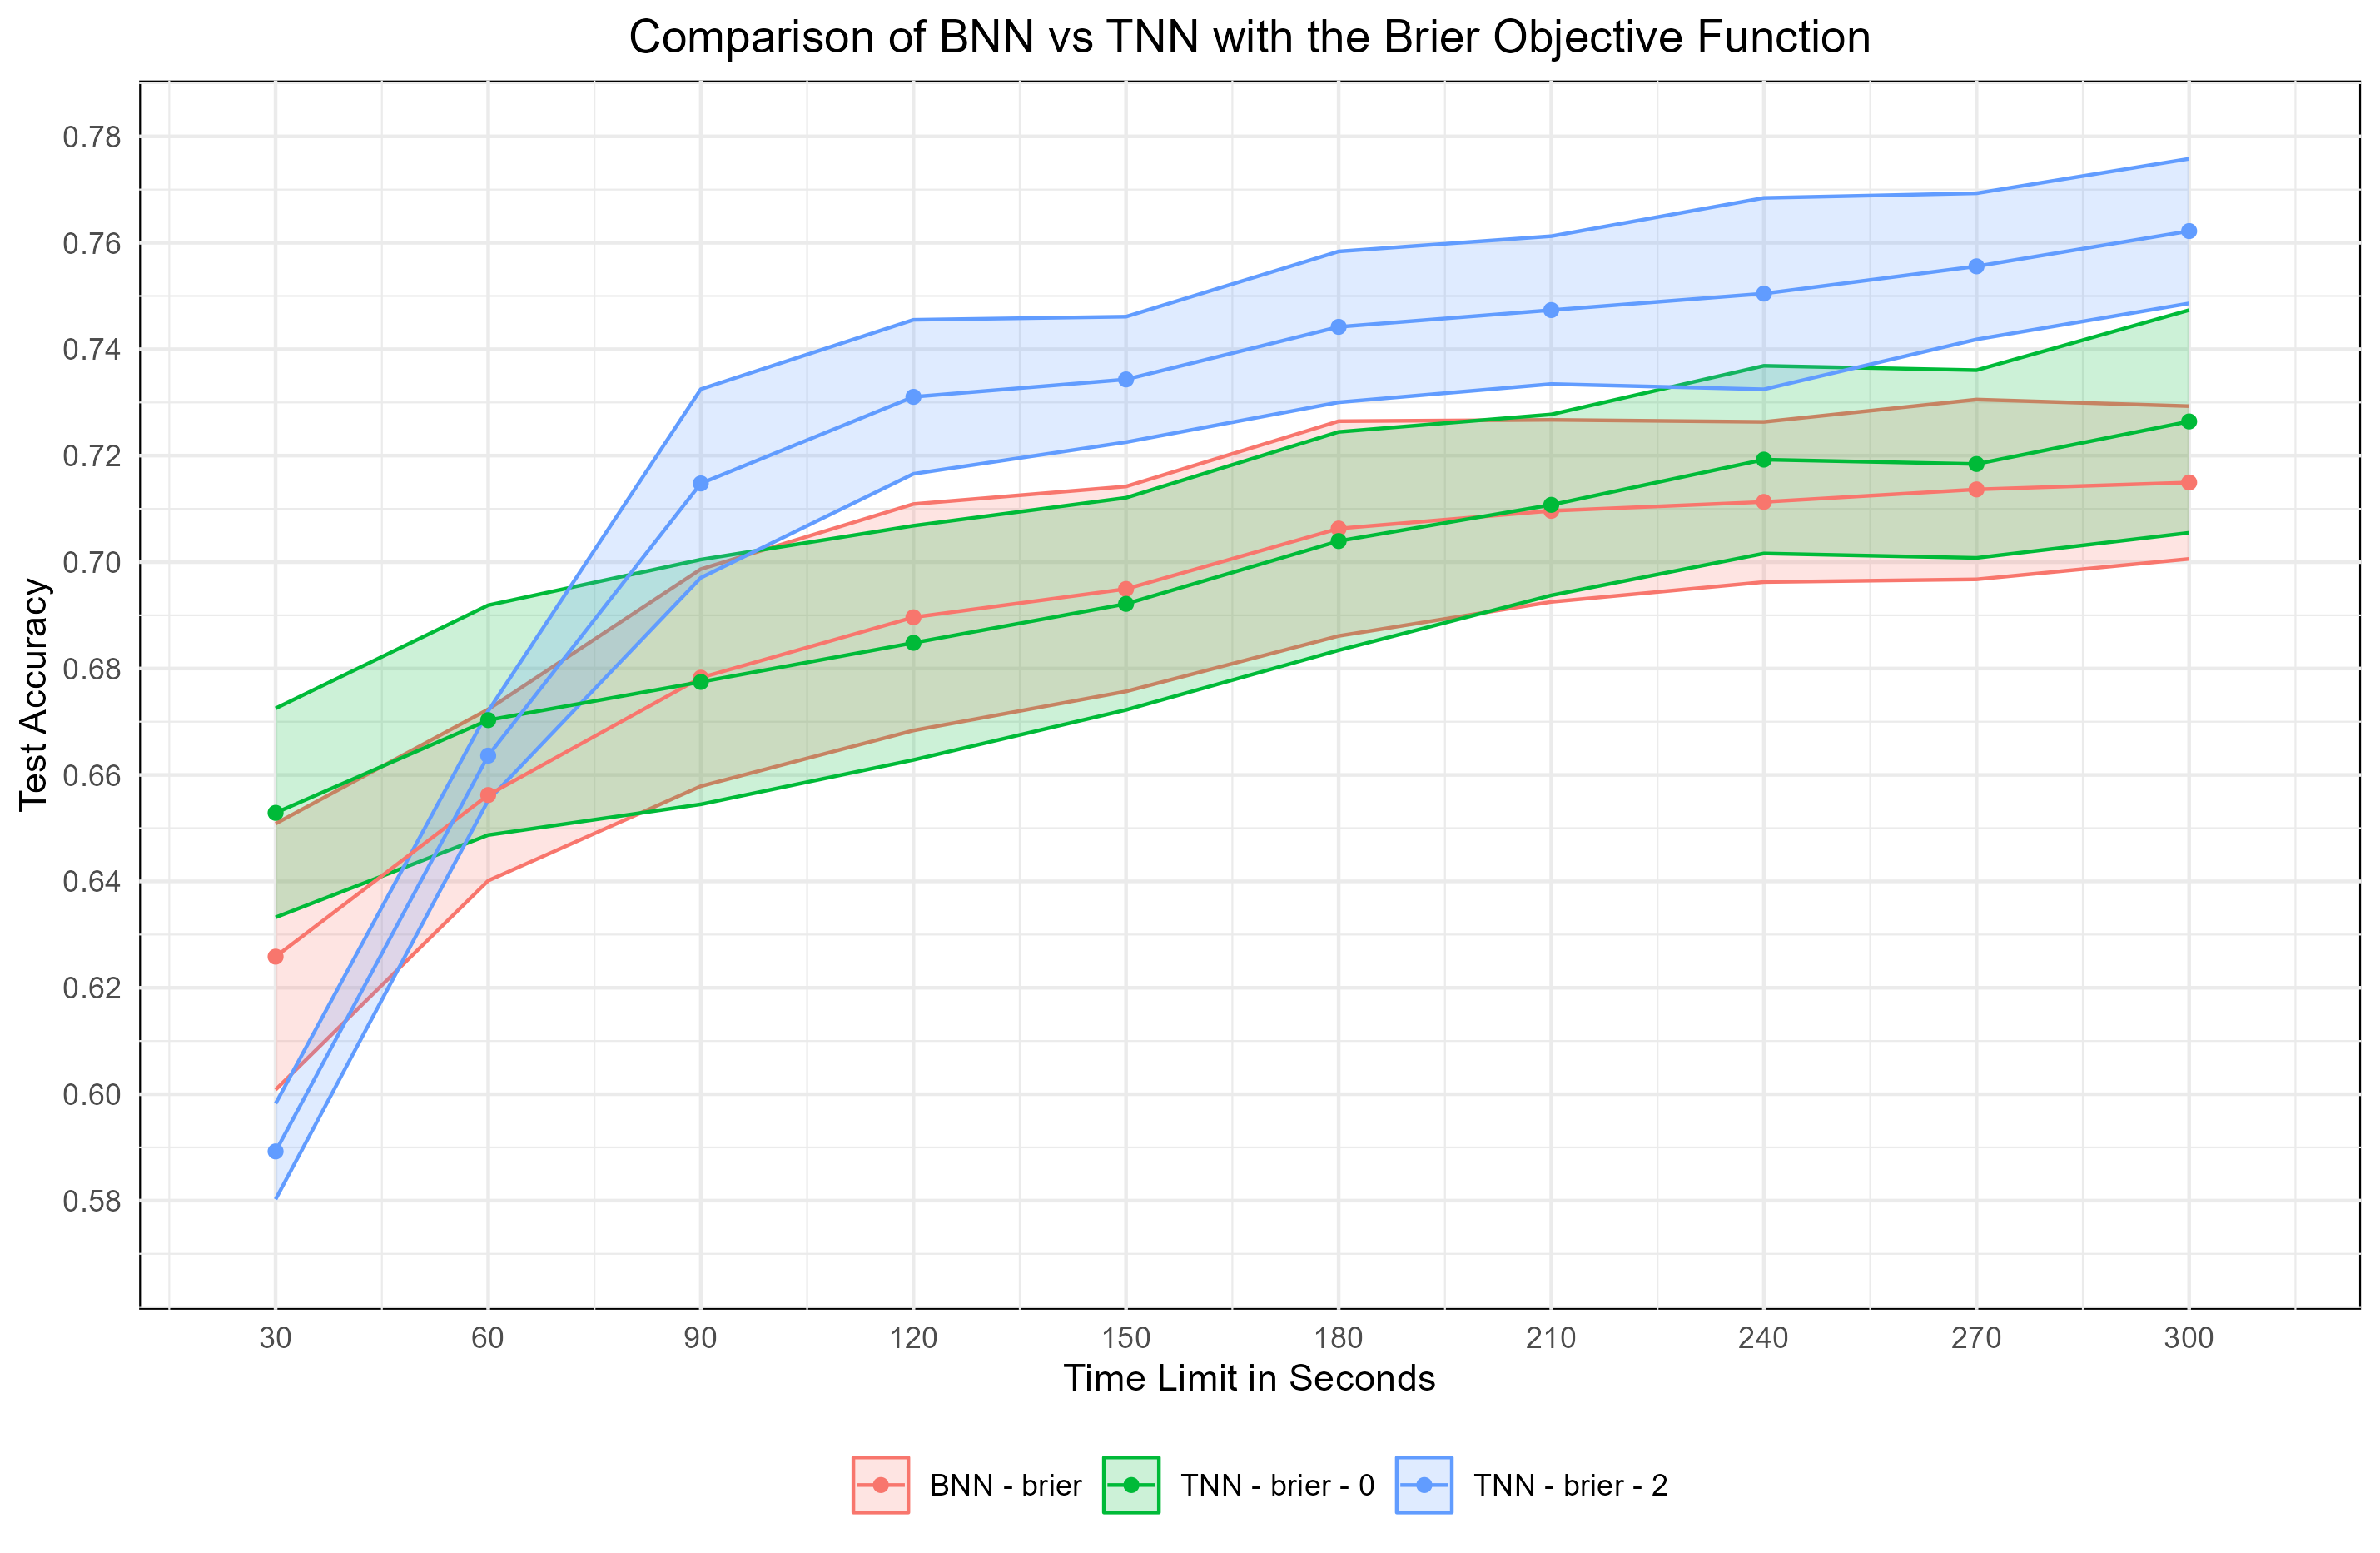
\includegraphics[width=1\linewidth]{Figures/BNN_vs_TNN_brier.png}
    \caption{\small{\textbf{Test accuracies for the MNIST dataset. The networks are trained on a single batch with 2000 samples, 200 for each digit. The results are for a neural network with a single hidden layer with 16 neurons. The labels indicate what type of network is trained and what the regularization parameter is. The figure shows the mean accuracy of 5 runs as a line and the standard deviation as a shaded area around it.}}}
    \label{BNN_vs_TNN_brier}
\end{figure}

\begin{figure}[H]
    \centering
    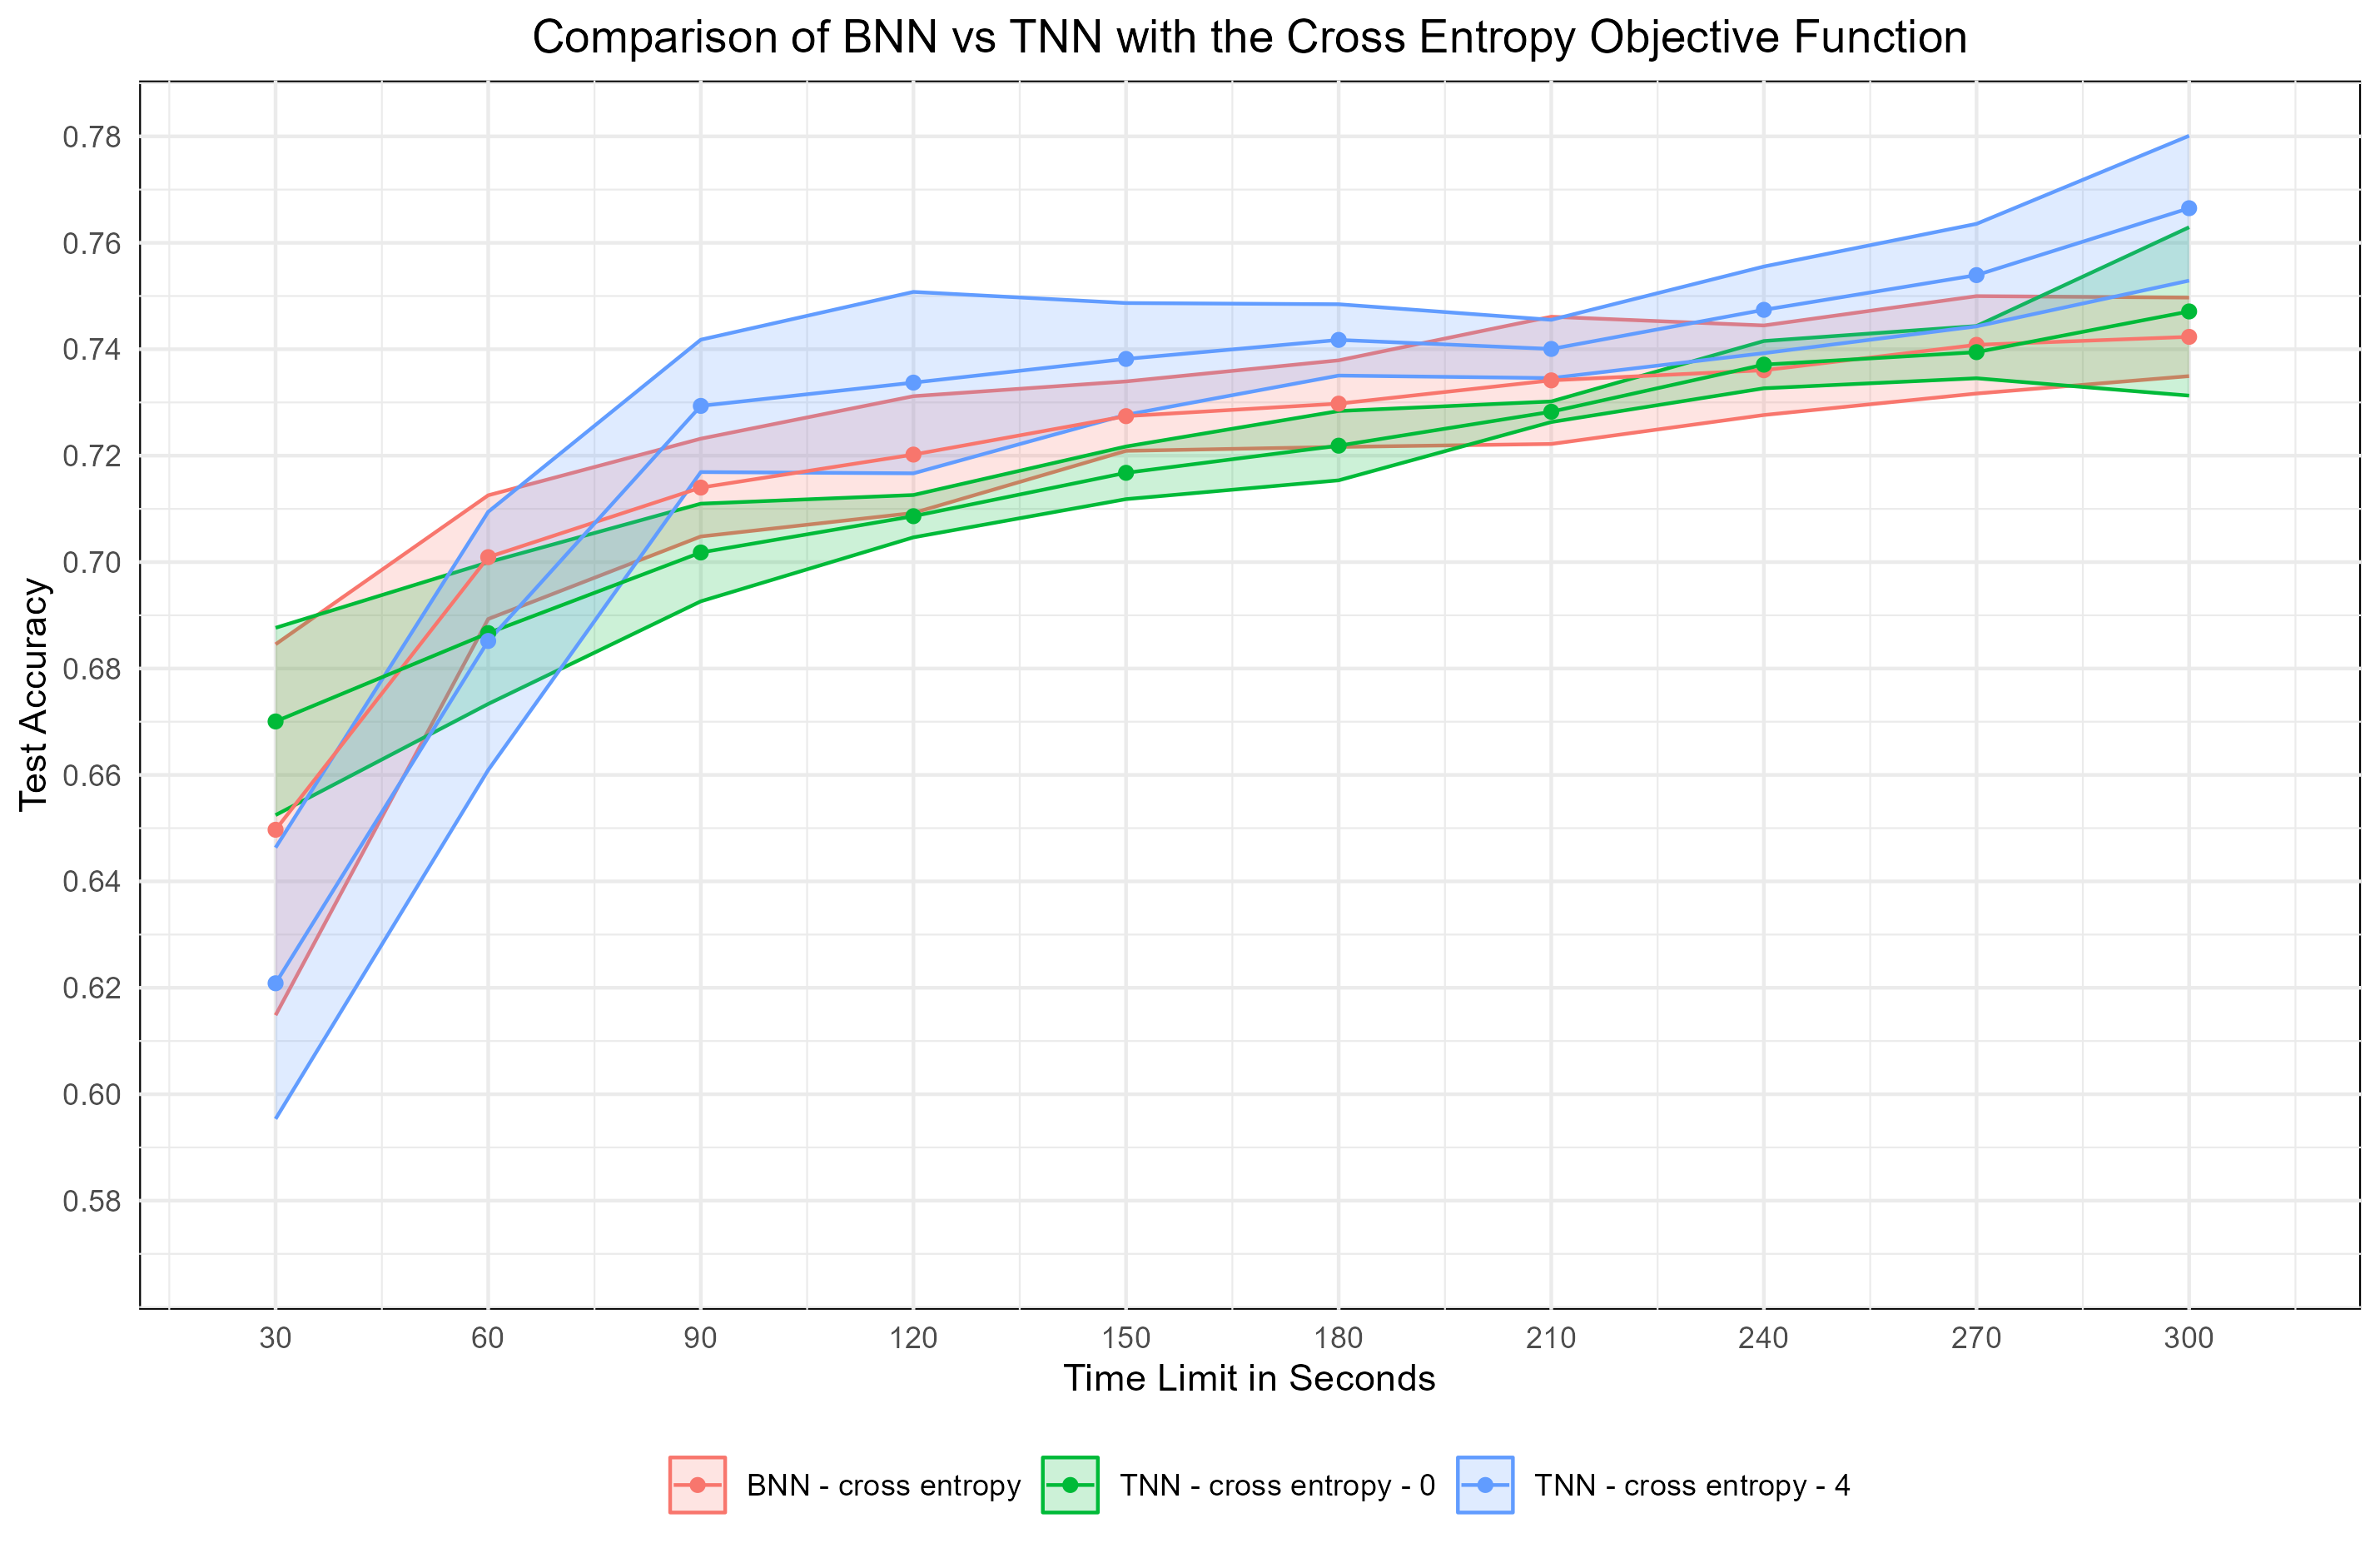
\includegraphics[width=1\linewidth]{Figures/BNN_vs_TNN_cs.png}
    \caption{\small{\textbf{Test accuracies for the MNIST dataset. The networks are trained on a single batch with 2000 samples, 200 for each digit. The results are for a neural network with a single hidden layer with 16 neurons. The labels indicate what type of network is trained and what the regularization parameter is. The figure shows the mean accuracy of 5 runs as a line and the standard deviation as a shaded area around it.}}}
    \label{BNN_vs_TNN_cs}
\end{figure}

\subsection{The BeMi Ensemble}
The implementation also supports training binary classifiers. As a result, it is possible to implement the BeMi ensemble introduced by \cite{ambrogio2023}. In their paper, they test their ensemble for two network architectures, both with two hidden layers. One of them has 4 neurons in both hidden layers, while the other has 10 in the first and 3 in the second. I will try to train networks with the same structure as them, i.e. 10 neurons in the first hidden layer and 3 in the second hidden layer. Besides this structure, I also train a network with a single hidden layer with 10 neurons. I hypothesize that this architecture is better, as the range of the preactivation values for the neuron in the last layer is larger. Recall that the BeMi ensemble works by training a binary classifier for each pair of classes. For MNIST, this means that 45 networks must be trained. Again, I use balanced batches to make a fair comparison against the existing literature. \cite{ambrogio2023} report their best average accuracy on MNIST to be 81.66 \%, using 40 images per digit and a total training time of 7.5 hours, as each of the 45 binary classifiers is trained for 600 seconds. \\

\noindent The remainder of this section is structured as follows: First I start by testing the different objective functions against each other. Afterwards, I explore the importance of training data and the effect of the time limit. Lastly, I move on from BNNs to TNNs and see if it is possible to improve on the BNN results. The original BeMi ensemble is trained on TNNs. 

\subsubsection{Comparing Objective Functions} 
For binary classifiers, there is only one neuron at the output layer, so across objective functions, the goal is the same, but the values of the objective functions can differ, which might lead to different results. I start by testing the different objective functions. I test with the two network architectures described above. I also test with both 10 and 100 images per digit and with a time limit for each binary classifier of 5 and 10 seconds. The results can be seen in Table \ref{BEMI_OBJ}, where, as expected, the objective functions give very similar results. For the network with a single hidden layer, the cross-entropy objective function gets the highest mean accuracies in 3 out of 4 cases, and in the fourth it is only beaten by 0.02 \% by the Brier objective function, which reaches a mean accuracy of 86.59 \% with 100 images per digit and 10 seconds of training time per classifier, a total training time of 450 seconds. For all configurations, the additional training time gives slightly better results, but in general the classifiers are much faster to train than in the work of \cite{ambrogio2023}, despite using more data. 

\begin{center}
% latex table generated in R 4.2.2 by xtable 1.8-4 package
% Fri May 31 11:29:08 2024
\begin{table}[H]
\centering
\begin{tabular}{|c|c|c|c|c|c|c|}
  \hline
ObjFunc & Images & Time & Mean1 & SD1 & Mean2 & SD2 \\ 
  \hline
brier & 100 & 225 & 0.5643 & 0.020748 & 0.3915 & 0.017008 \\ 
   \hline
brier & 100 & 450 & 0.5766 & 0.024475 & 0.3857 & 0.035266 \\ 
   \hline
brier & 1000 & 225 & 0.8569 & 0.004764 & 0.7417 & 0.010035 \\ 
   \hline
brier & 1000 & 450 & 0.8659 & 0.004340 & 0.7470 & 0.013553 \\ 
   \hline
cross-entropy & 100 & 225 & 0.5708 & 0.028872 & 0.3720 & 0.021409 \\ 
   \hline
cross-entropy & 100 & 450 & 0.5851 & 0.029226 & 0.3735 & 0.011863 \\ 
   \hline
cross-entropy & 1000 & 225 & 0.8582 & 0.007717 & 0.7442 & 0.017460 \\ 
   \hline
cross-entropy & 1000 & 450 & 0.8657 & 0.005599 & 0.7483 & 0.012503 \\ 
   \hline
integer & 100 & 225 & 0.5709 & 0.029312 & 0.3733 & 0.025777 \\ 
   \hline
integer & 100 & 450 & 0.5804 & 0.029027 & 0.3844 & 0.015866 \\ 
   \hline
integer & 1000 & 225 & 0.8580 & 0.005094 & 0.7282 & 0.010162 \\ 
   \hline
integer & 1000 & 450 & 0.8633 & 0.004024 & 0.7287 & 0.009162 \\ 
   \hline
\end{tabular}
\caption{Mean accuracies for the BeMi ensemble. Mean1 and SD1 is for a BNN with a single hidden layer with
          10 neurons. Mean2 and SD2 is for a BNN with a hidden layer with 10 neurons followed by a hidden layer
          with 3 neurons. The training time is the total training time, so each of the 45 networks are trained for
          5 and 10 seconds respectively. The number of images, is the total number of images, so there is 10
          and 100 images for each digit respectively. } 
\label{BEMI_OBJ}
\end{table}

\end{center}


\subsubsection{Testing the Effect of More Training Data}
One of the limitations of the MIP model that the BeMi ensemble was originally trained on is the amount of data it can handle. In a LS context, this limitation does not apply in the same way, so it is possible to train on more training data. Figure \ref{BEMI_BS} shows the importance of more training data, as the test accuracy quickly increases. The figure is with a time limit of only 5 seconds, so it is highly likely that increasing the time limit will yield even higher accuracies. With 40 images per digit, corresponding to the amount of data \cite{ambrogio2023} use for their best result (81.66 \%), I get a mean accuracy in this experiment of 79.84 \%, despite using way less time than them. It should be noted, that their result was for the network architecture with two hidden layers with only 4 neurons in each, but they do not get a higher accuracy when using the network architecture with 10 neurons in the first hidden layer and 3 in the second. I only use a single hidden layer with 10 neurons, which does not make the network larger compared to their second architecture. Another thing to notice is that I use a BNN in this experiment, so besides the objective function, I do not in any way regularize the model or train it to be more robust. 

\begin{figure}[H]
    \centering
    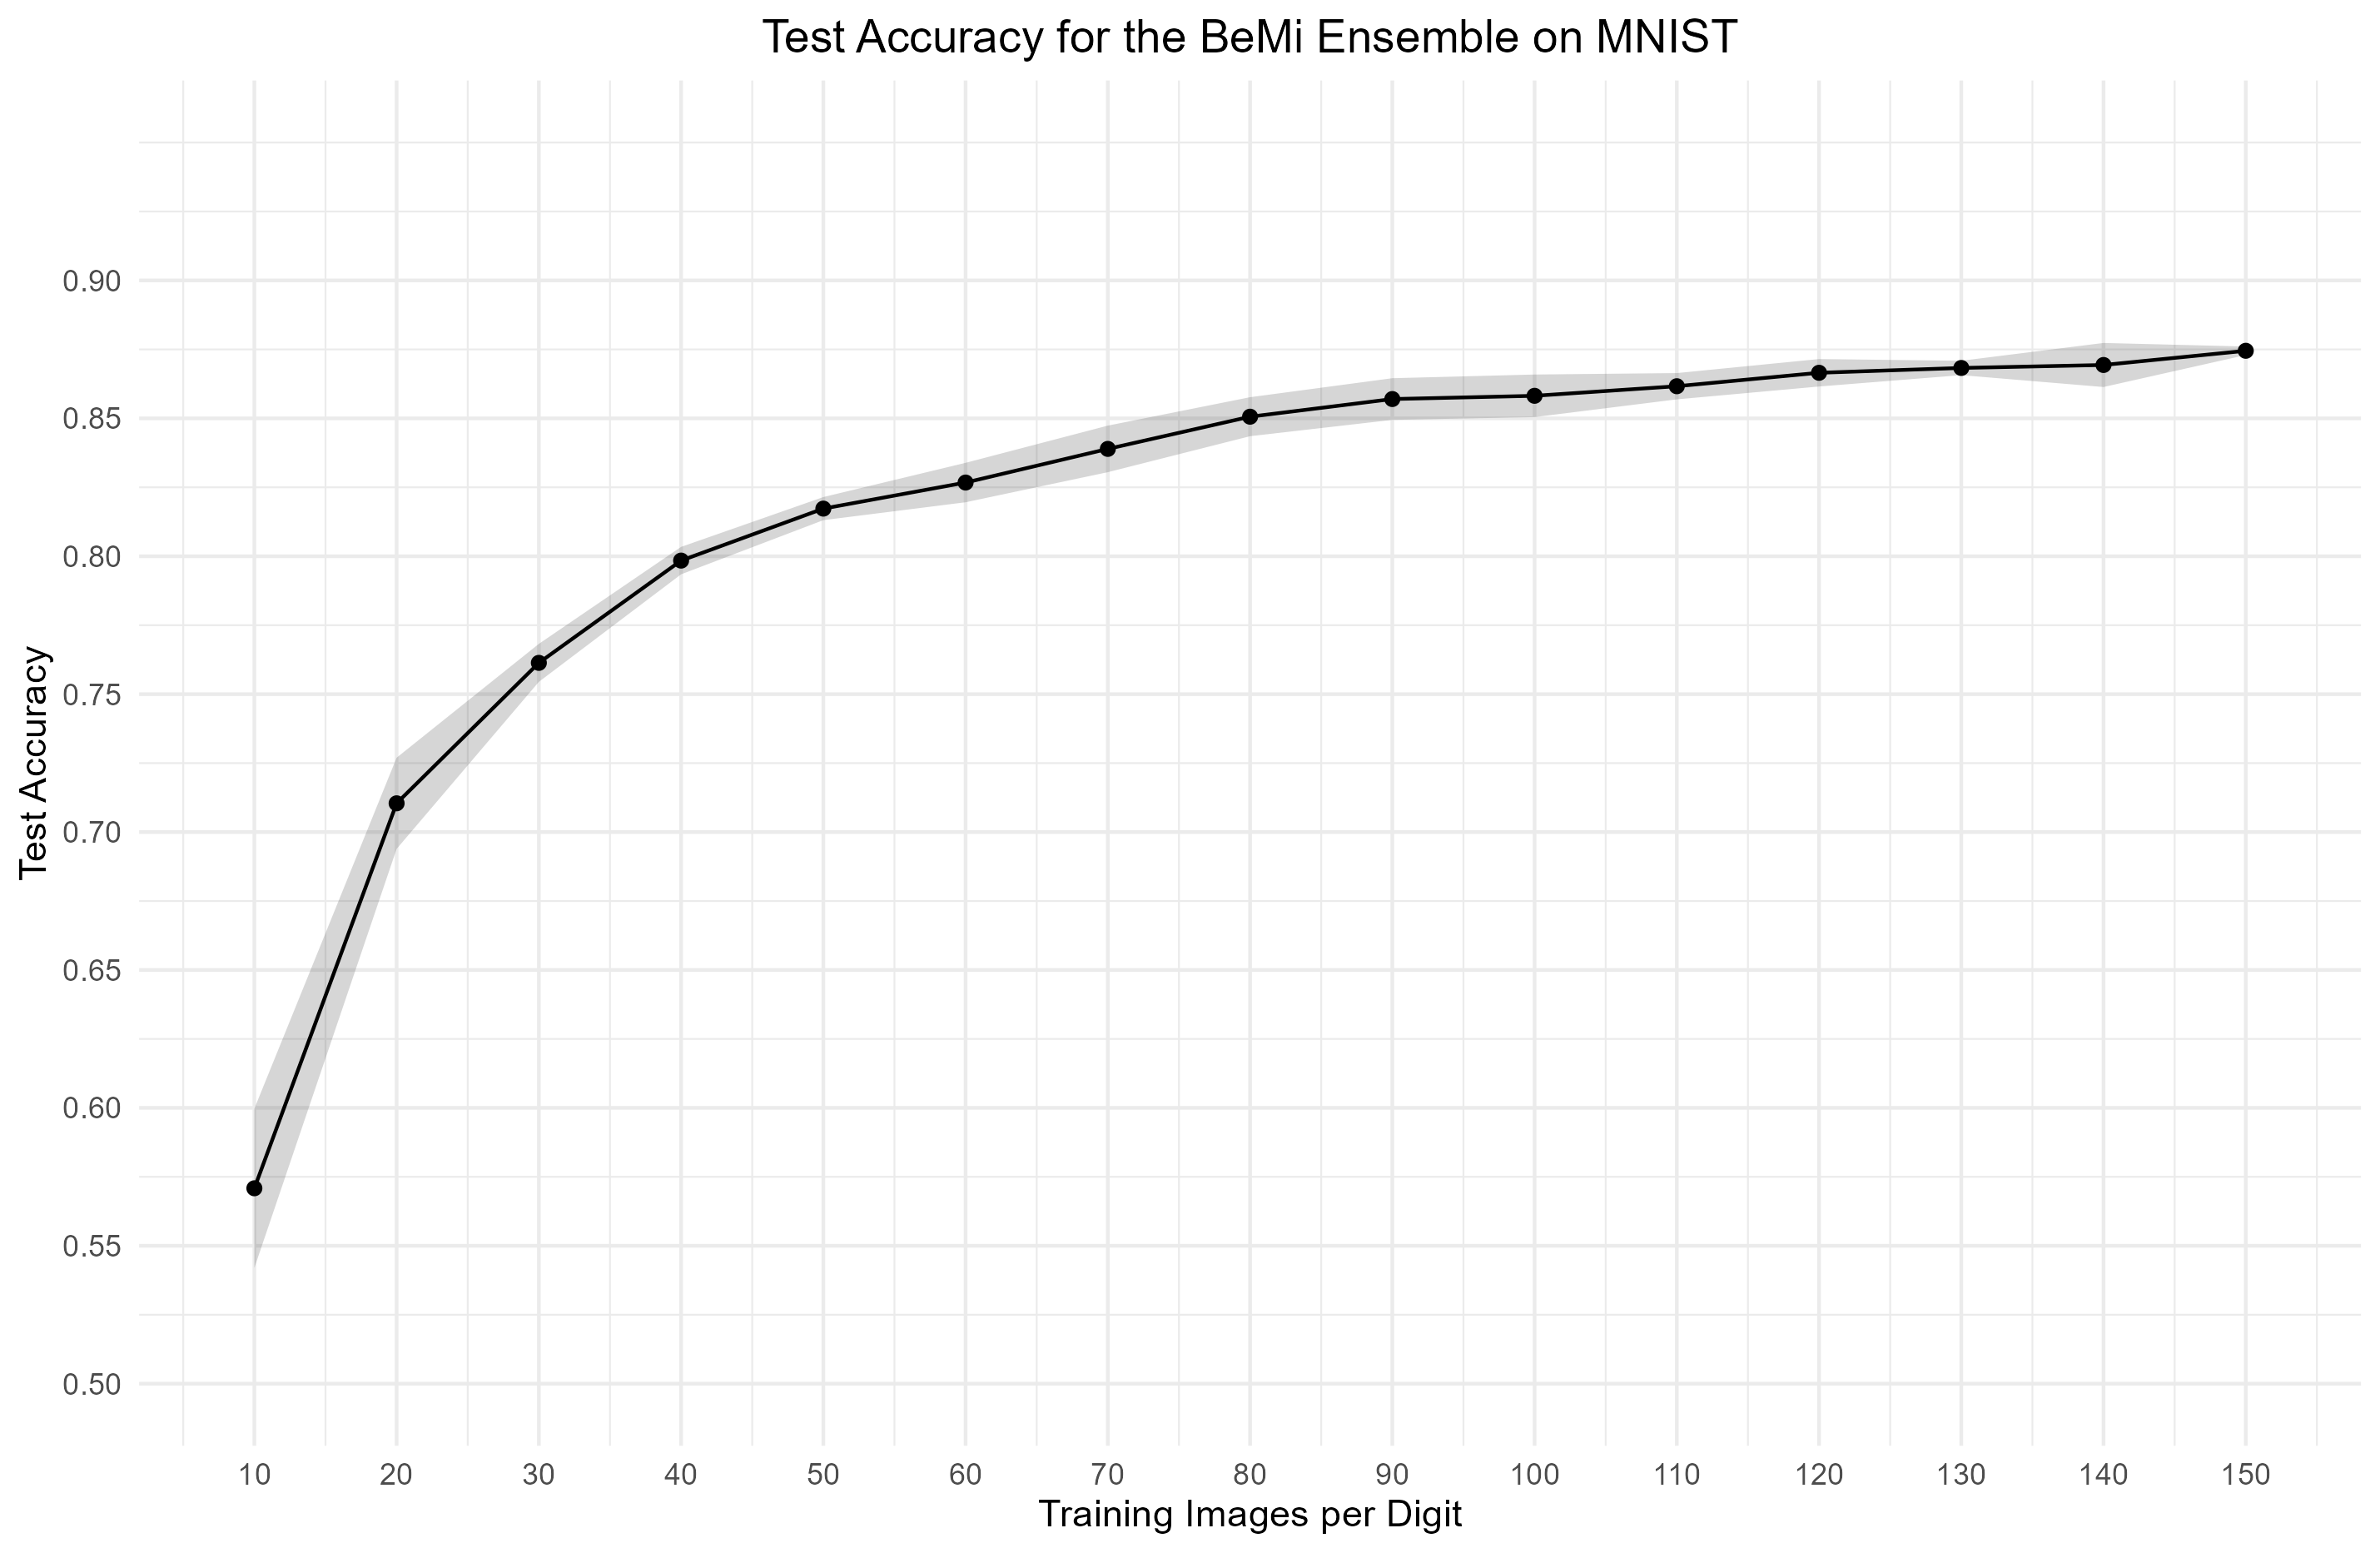
\includegraphics[width=1\linewidth]{Figures/BEMI_BS.png}
    \caption{\small{\textbf{The test accuracy on MNIST for the BeMi ensemble as the amount of training data increases. The network is a BNN with a single hidden layer with 10 neurons.
    Each binary classifier is trained for 5 seconds, giving a total training time of 225 seconds. Cross-entropy is used as objective function.}}}
    \label{BEMI_BS}
\end{figure}

\subsubsection{Testing the Effect of the Time Limit}
To test how much the results improve as the time limit increases, I fix the amount of training data to 100 images per digit and let the time limit vary. Table \ref{BEMI_TIME} shows that increasing the time limit improves the accuracy slightly and the standard deviation decreases, so the results become more stable. 

\begin{center}
% latex table generated in R 4.2.2 by xtable 1.8-4 package
% Fri May 31 11:47:23 2024
\begin{table}[H]
\centering
\begin{tabular}{|c|c|c|}
  \hline
TrainingTime & Mean & SD \\ 
  \hline
225.00 & 0.8568 & 0.006649 \\ 
   \hline
450.00 & 0.8657 & 0.005599 \\ 
   \hline
675.00 & 0.8669 & 0.005870 \\ 
   \hline
900.00 & 0.8684 & 0.005119 \\ 
   \hline
\end{tabular}
\caption{Summary statistics for the BeMi ensemble for different time limits. The
          network is a BNN with a single hidden layer with 10 neurons and the training is based on
          100 images per digit. I use cross entropy as objective function. } 
\label{BEMI_TIME}
\end{table}

\end{center}


\subsubsection{Using Ternary Neural Networks in the BeMi Ensemble}
As mentioned earlier, in their original publication of the BeMi ensemble, \cite{ambrogio2023} used TNNs for their binary classifiers. So far, I have only used BNNs, but in this section I also try with TNNs. I experiment with different perturbation sizes as well as different weights for the regularization parameter. Table \ref{BEMI_TNN} presents the results for this experiment, and even though the capacity of the model should increase, none of the configurations produce better results than the best one achieved in Table \ref{BEMI_TIME}, where the maximum mean accuracy was 86.84 \%. Further, it does not seem to be the case that adding a regularization parameter helps. It might be that the best weight for the regularization parameter has not been found. The experiments earlier (Table \ref{TNN_COF}, \ref{TNN_REG_BRIER}, \ref{TNN_REG_CS}, and \ref{TNN_REG_INT}) showed how difficult it is to find an optimal regularization parameter. 

\begin{center}
% latex table generated in R 4.2.2 by xtable 1.8-4 package
% Sun Jun  2 22:08:24 2024
\begin{table}[H]
\centering
\begin{tabular}{|c|c|c|c|}
  \hline
Reg & PS & Mean & SD \\ 
  \hline
0.0000 &  10 & 0.8585 & 0.0070 \\ 
   \hline
0.0000 &  30 & 0.8673 & 0.0059 \\ 
   \hline
0.0000 &  50 & 0.8679 & 0.0031 \\ 
   \hline
0.0001 &  10 & 0.8489 & 0.0053 \\ 
   \hline
0.0001 &  30 & 0.8529 & 0.0042 \\ 
   \hline
0.0001 &  50 & 0.8528 & 0.0030 \\ 
   \hline
0.0010 &  10 & 0.8510 & 0.0028 \\ 
   \hline
0.0010 &  30 & 0.8509 & 0.0048 \\ 
   \hline
0.0010 &  50 & 0.8517 & 0.0046 \\ 
   \hline
0.0100 &  10 & 0.8449 & 0.0056 \\ 
   \hline
0.0100 &  30 & 0.8489 & 0.0024 \\ 
   \hline
0.0100 &  50 & 0.8446 & 0.0088 \\ 
   \hline
\end{tabular}
\caption{\small{\textbf{Summary statistics for the BeMi ensemble on MNIST when trained with different perturbation sizes and 
          different regularization parameters. The networks trained has a single hidden layer with 10 neurons and is trained for
          20 seconds each, so the total training time is 900 seconds.}}} 
\label{BEMI_TNN}
\end{table}

\end{center}

\subsection{Testing on Other Datasets}
So far, I have only trained on the MNIST dataset. In this section, I will train on two other datasets as well, namely the more challenging Fashion-MNIST (FMNIST) dataset and the Adult dataset. The structure of the FMNIST dataset is the same as for the MNIST. The training set has 60,000 examples and the test set has 10,000 examples. Each example is a $28 \times 28$ grayscale image, but whereas the MNIST dataset consists of handwritten digits, the FMNIST dataset consists of images of Zalando articles divided into 10 classes. The task with the Adult dataset is to predict whether the income of an individual exceeds 50,000 dollars a year based on census data. This dataset has 14 features, but since some of them are categorical, the number of inputs to the neural network is 104 after standardizing the features. I will repeat some of the experiments conducted so far for these datasets to see if the conclusions drawn so far generalize to these datasets as well. 
\begin{center}
% latex table generated in R 4.2.2 by xtable 1.8-4 package
% Sun Jun  2 00:23:15 2024
\begin{table}[!b]
\centering
\begin{tabular}{|c|c|c|c|}
  \hline
ObjectiveFunction & Neurons & Mean & SD \\ 
  \hline
brier & 16 & 0.7016 & 0.0040 \\ 
   \hline
cross-entropy & 16 & 0.6891 & 0.0250 \\ 
   \hline
integer & 16 & 0.6977 & 0.0590 \\ 
   \hline
brier & 128 & 0.6426 & 0.0492 \\ 
   \hline
cross-entropy & 128 & 0.7434 & 0.0060 \\ 
   \hline
integer & 128 & 0.7215 & 0.0115 \\ 
   \hline
\end{tabular}
\caption{\small{\textbf{The mean test accuracies on Fashion-MNIST for different network structures. The results are obtained by training a BNN
            on a single batch with 2000 samples using the ILS algorithm with a time limit of 300 seconds.
            The network is a BNN with a single hidden layer with the number of neurons indicated by the 'Neurons' column.}}} 
\label{SBT_DNS_FMNIST}
\end{table}

\end{center}

\subsubsection{Results on the Fashion-MNIST Dataset}

For the FMNIST dataset, I start by running an experiment on a single batch setting similar to Table \ref{SBT_DNS}. This time, I only use one hidden layer, but I still test three objective functions. I train on 2,000 examples. Table \ref{SBT_DNS_FMNIST} presents the results for the FMNIST dataset. For the MNIST case, it was the cross-entropy objective function that performed best with a small network architecture, whereas for the FMNIST, the Brier objective function performs a little better. For the large network architecture, it is, however, again the cross-entropy function that performs best. \\

\noindent I also replicate the multiple batch training experiment producing Table \ref{MBT}, but this time for the FMNIST dataset. The results can be seen in Table \ref{MBT_FMNIST} and it shows many of the similar patterns as Table \ref{MBT}. First of all, the results show that the FMNIST dataset, as expected, is more challenging than the standard MNIST, as the mean accuracies are generally lower. This time, the integer objective function performs significantly worse on small networks. The reason for this could be, as indicated earlier, that the integer objective function does not directly work with probabilities, and since the classes in this dataset are more difficult to distinguish from each other, the small networks with 16 neurons in the hidden layers are too small to work well for the integer objective function. For the large network architecture with 128 neurons in the hidden layers, it is, however, again the integer objective function that performs best. Overall, it is again the aggregation algorithm that gives the best results. The maximum mean accuracy obtained is 82.66 \% for the integer objective function with the aggregation algorithm and a network with two hidden layers with 128 neurons. 

\noindent As a last experiment for the FMNIST dataset, I also try with the BeMi ensemble, but this time only with a network architecture with a single hidden layer with 10 neurons. I only train a BNN. The best accuracy achieved by \cite{ambrogio2023} on this dataset is slightly above 70 \%. They do not present this result in a table, but in a figure, so the exact number cannot be reported. Again, they train the ensemble for 7,5 hours, whereas I only train for 15 minutes. The results I obtain are summarized in Table \ref{BEMI_OBJ_FMNIST}. For the same amount of data as \cite{ambrogio2023}, I achieve a higher accuracy for all three objective functions, and with more data, the results only get better. The reason for achieving a higher accuracy is probably due to a combination of using a single hidden layer, so the range of the preactivation values in the output neuron is larger, and that the objective functions I can use in a local search context do a better job of making sure that the model is robust. 
\begin{center}
% latex table generated in R 4.2.2 by xtable 1.8-4 package
% Sat Jun  1 18:09:47 2024
\begin{table}[!tb]
\centering
\begin{tabular}{|c|c|c|c|c|}
  \hline
Objective function & Hidden layers & Algorithm & 16 & 128 \\ 
  \hline
brier & One & Iterated Improvement & 0.7670 & 0.7667 \\ 
   \hline
brier & One & Aggregation Algorithm & 0.7644 & 0.8056 \\ 
   \hline
brier & One & Iterated Local Search & 0.7471 & 0.7749 \\ 
   \hline
cross-entropy & One & Iterated Improvement & 0.7295 & 0.7596 \\ 
   \hline
cross-entropy & One & Aggregation Algorithm & 0.7236 & 0.7531 \\ 
   \hline
cross-entropy & One & Iterated Local Search & 0.7188 & 0.7673 \\ 
   \hline
integer & One & Iterated Improvement & 0.6709 & 0.7951 \\ 
   \hline
integer & One & Aggregation Algorithm & 0.5622 & 0.8058 \\ 
   \hline
integer & One & Iterated Local Search & 0.7314 & 0.7889 \\ 
   \hline
brier & Two & Iterated Improvement & 0.7220 & 0.6312 \\ 
   \hline
brier & Two & Aggregation Algorithm & 0.5324 & 0.7691 \\ 
   \hline
brier & Two & Iterated Local Search & 0.6948 & 0.6639 \\ 
   \hline
cross-entropy & Two & Iterated Improvement & 0.6956 & 0.6550 \\ 
   \hline
cross-entropy & Two & Aggregation Algorithm & 0.6125 & 0.7061 \\ 
   \hline
cross-entropy & Two & Iterated Local Search & 0.6764 & 0.6756 \\ 
   \hline
integer & Two & Iterated Improvement & 0.5507 & 0.8090 \\ 
   \hline
integer & Two & Aggregation Algorithm & 0.4947 & 0.8266 \\ 
   \hline
integer & Two & Iterated Local Search & 0.6776 & 0.8058 \\ 
   \hline
\end{tabular}
\caption{\small{\textbf{The mean test accuracies on Fashion-MNIST for different network structures and algorithms. The network is a
            BNN trained with a time limit of 600 seconds. Iterated Improvement and Iterated Local Search refers to
            Algorithm 4, and here early stopping is used. The validation dataset is 12,000 samples and for
            II, the validation accuracy is calculated every fourth batch, whereas for ILS, it is after every batch.
            The solution with the highest validation accuracy is returned. I set bp equal to 1 and ps to 25.
            Each ILS phase is allowed to run for 5 seconds. 
            For the Aggregation Algorithm, I do not use early stopping, but return the solution at the end. The parameters
            updateStart, updateEnd and updateIncrease are set to 1, 15 and 10 respectively. For all the algorithms
            a batch size of 1000 is used.}}} 
\label{MBT_FMNIST}
\end{table}

\end{center}

\begin{center}
% latex table generated in R 4.2.2 by xtable 1.8-4 package
% Sat Jun  1 18:29:25 2024
\begin{table}[!tb]
\centering
\begin{tabular}{|c|c|c|c|}
  \hline
ObjFunc & Images & Mean & SD \\ 
  \hline
brier & 400 & 0.7287 & 0.007214 \\ 
   \hline
brier & 1000 & 0.7633 & 0.003263 \\ 
   \hline
cross-entropy & 400 & 0.7337 & 0.001938 \\ 
   \hline
cross-entropy & 1000 & 0.7635 & 0.003819 \\ 
   \hline
integer & 400 & 0.7239 & 0.005019 \\ 
   \hline
integer & 1000 & 0.7738 & 0.007698 \\ 
   \hline
\end{tabular}
\caption{\small{\textbf{Mean accuracies for the BeMi ensemble on the Fashion-MNIST dataset. The networks
          have a single hidden layer with 10 neurons and are trained for 20 seconds each, giving a total
          training time of 900 seconds. The number of images is the total number of images, so there is
          40 and 100 images for each digit respectively.}}} 
\label{BEMI_OBJ_FMNIST}
\end{table}

\end{center}


\subsubsection{Results on the Adult Dataset}
The Adult dataset, which can be imported into Python using: https://pypi.org/project/adult-dataset/, has 30162 training examples and 15060 test examples. As mentioned earlier, this dataset is different from the MNIST datasets, as it does not deal with image classification. The number of inputs is only 104 after standardizing the features. \cite{thorbjarnason2023} test their model on the Adult dataset in two different experiments. In one of their experiments, they use a model that simultaneously trains the neural network and minimizes the number of neurons needed. They do this by allowing the network to have a maximum of 16 neurons in the hidden layer and then they have a weight that serves as a regularizer. With 800 training examples and a running time of 10 hours, their best reported result has a mean test accuracy of 78.8 \% and on average 5.2 neurons are in the hidden layer. They use integer neural networks, wherein the values of the weights can take on any value between $\{-15, \ldots, 15\}$, whereas I only work with BNNs and TNNs. \\

\noindent While my model cannot minimize the number of neurons, it can, for a TNN, minimize the number of active connections. Using the same amount of data and only a time limit of 60 seconds, I achieve higher accuracy than the results from \cite{thorbjarnason2023}. In Table \ref{TNN_COF_Adult}, the results can be seen for single batch training. The integer objective function works best, but for small weights of the regularization parameter, it does not regularize as much as the other objective functions. Nevertheless, with a small regularization weight, the integer objective function reaches a mean accuracy of 82.44 \% with 560 connections on average being active in the network. The total number of connections in the network is 1680. \\

\noindent \cite{thorbjarnason2023} also train a neural network using their batch training method on the Adult dataset. Their model with this procedure reaches a mean accuracy of 83.8\% and the average runtime is 18900 seconds. Table \ref{MBT_REG_Adult} shows my results when I train a ternary neural network on multiple batches. I use the integer objective function and the aggregation algorithm. Even though I only train for 90 seconds, and the network I use is only a TNN, I achieve a mean accuracy of 83.88 \%. The number of active connections is also lower now compared to before, even though the regularization parameter is the same. 

\begin{center}
% latex table generated in R 4.2.2 by xtable 1.8-4 package
% Sat Jun  1 23:42:43 2024
\begin{table}[!tb]
\centering
\begin{tabular}{|c|c|c|c|c|c|}
  \hline
Reg & ObjectiveFunc & Mean & SD & Connections & LocalOptimas \\ 
  \hline
0.00 & brier & 0.8060 & 0.0030 & 1207 & 119 \\ 
   \hline
0.10 & brier & 0.8047 & 0.0050 &  253 & 100 \\ 
   \hline
0.25 & brier & 0.8155 & 0.0023 &  113 & 121 \\ 
   \hline
0.50 & brier & 0.8102 & 0.0096 &   62 & 146 \\ 
   \hline
1.00 & brier & 0.8003 & 0.0210 &   19 & 172 \\ 
   \hline
0.00 & cross-entropy & 0.8032 & 0.0086 & 1203 & 117 \\ 
   \hline
0.10 & cross-entropy & 0.7961 & 0.0135 &  398 &  75 \\ 
   \hline
0.25 & cross-entropy & 0.8036 & 0.0154 &  316 &  94 \\ 
   \hline
0.50 & cross-entropy & 0.7988 & 0.0096 &  196 & 106 \\ 
   \hline
1.00 & cross-entropy & 0.8073 & 0.0105 &   79 & 132 \\ 
   \hline
0.00 & integer & 0.8219 & 0.0061 & 1161 & 245 \\ 
   \hline
0.10 & integer & 0.8241 & 0.0064 &  567 & 148 \\ 
   \hline
0.25 & integer & 0.8240 & 0.0064 &  567 & 147 \\ 
   \hline
0.50 & integer & 0.8244 & 0.0064 &  560 & 150 \\ 
   \hline
1.00 & integer & 0.8234 & 0.0058 &  518 & 150 \\ 
   \hline
\end{tabular}
\caption{\small{\textbf{Summary statistics for single batch training of a TNN with 800 examples from the Adult dataset. 
          The network trained has a single hidden layer with 16 neurons and is trained for
          60 seconds.}}} 
\label{TNN_COF_Adult}
\end{table}

\end{center}

\begin{center}
% latex table generated in R 4.2.2 by xtable 1.8-4 package
% Sun Jun  2 22:30:24 2024
\begin{table}[!tb]
\centering
\begin{tabular}{|c|c|c|c|}
  \hline
Reg & Mean & SD & Connections \\ 
  \hline
 0.0 & 0.8381 & 0.0016 & 1105 \\ 
   \hline
 0.5 & 0.8388 & 0.0014 &  419 \\ 
   \hline
 2.0 & 0.8333 & 0.0013 &  214 \\ 
   \hline
 4.0 & 0.8306 & 0.0016 &  152 \\ 
   \hline
 6.0 & 0.8296 & 0.0033 &  134 \\ 
   \hline
 8.0 & 0.8249 & 0.0041 &  115 \\ 
   \hline
10.0 & 0.8213 & 0.0031 &  105 \\ 
   \hline
\end{tabular}
\caption{\small{\textbf{Summary statistics for the aggregation algorithm with the integer objective function trained on the Adult
            dataset. The algorithm runs for 90 seconds and the network is a TNN with different 
            regularization parameters. The network has a single hidden layer with 16 neurons. The batch size
            is 800, updateStart is 1, updateEnd 20 and updateIncrease is 10.}}} 
\label{MBT_REG_Adult}
\end{table}

\end{center}




\newpage
\section{Conclusion and Future Work}
In this thesis, I investigated the feasibility of training binary and ternary neural networks using local search methods. By efficiently utilizing the discrete nature of these networks, I implemented an efficient delta evaluation, enabling the training of networks within small time limits compared to existing MIP methods for training few-bits neural networks. \\

\noindent Existing work on training binary and ternary neural networks using MIP models has primarily focused on few-shot learning with small network architectures due to their high training time, which limits scalability. In contrast, the local search procedure presented in this thesis scales well with increased data and larger networks. For instance, I demonstrated that the BeMi ensemble introduced by \cite{ambrogio2023} can achieve higher accuracy than previously reported by training on more data, making it very suitable for few-shot learning. Specifically, with 1,000 training examples, the emsemble achieved a mean accuracy of 86.84\% on the MNIST dataset. This significant improvement over the 81\% they reported can be attributed to two main factors: the use of additional data and the omission of one of the two hidden layers, which widened the range of the preactivation values. The 86.84\% achieved with the BeMi ensemble also surpasses the results from training on a single batch of data with 2,000 training examples and a network with a single hidden layer of 128 neurons, where the maximum mean accuracy was only 81.85 \%. The BeMi ensemble outperforms this result with half the data, and a similar pattern is observed on the more challenging Fashion-MNIST dataset. \\

\noindent In addition to focusing on few-shot learning, this work proposes several algorithms capable of training on multiple batches, thereby enabling the use of much larger datasets. Among these, the aggregation algorithm showed great potential. Unlike the other proposed methods that adjust weights based on a single batch of samples, this algorithm calculates delta values for multiple batches, aggregates them, and adjusts the weights based on the aggregated values. This approach helps ensure better generalization of the model. The aggregation algorithm facilitated the training of larger networks, where the proposed integer objective function outperformed the standard cross-entropy loss function and the Brier score objective function. Specifically, the integer objective function demonstrated reduced overfitting compared to the other objective functions. However, a notable drawback is that this objective function does not always perform well with small network architectures, as it does not handle probabilities in the same way as the other functions. \\

\noindent The aggregation algorithm, combined with the integer objective function, achieved a test accuracy of 91.53\% on the MNIST dataset using a neural network with two hidden layers, each containing 128 neurons. While this result is promising, it is important to note that a significant gap remains compared to state-of-the-art binary neural network training methods that employ more traditional approaches. Despite this gap, the success of the aggregation algorithm and integer objective function in reaching high accuracy with relatively simple network architectures demonstrates their potential. These methods offer an alternative approach that can be particularly advantageous in scenarios where computational resources are limited. \\

\noindent With the increasing use of AI in real-world applications, binary and ternary neural networks are gaining significant attention. These networks are particularly valuable in computationally limited and energy-constrained devices. Binary and ternary neural networks show great potential in these environments due to their reduced computational complexity and lower power consumption compared to traditional floating-point neural networks. However, a performance gap often exists when working with discrete neural networks compared to their floating-point counterparts. This performance gap is also observed in this thesis. Nevertheless, the local search framework developed provides a promising foundation for narrowing this gap. \\

\noindent Future work can go in several directions. While this implementation uses Python, it would be interesting to investigate whether the running time could be reduced by implementing the algorithms in a language supporting more optimized code development, such as C++. C++ is closer to the hardware and it is in general faster than Python, but it does not have the same large standard libraries as Python and is considered more difficult to learn than Python. \\

\noindent It is also possible that the proposed algorithms, such as the aggregation algorithm can be expanded further. It would be interesting to investigate whether a perturbation strategy could help the model get to an even better solution. It might also be the case that the algorithm takes too many moves at once. The delta evaluation is always calculated under the assumption that it is only the value of that weight that changes. The aggregation algorithms commit many moves at once and as a result it is a possibility, especially later on in the algorithm, that the committed moves in a way cancels each other out. \\

\noindent As mentioned, the delta evaluation assumes only one weight changes at a time. In a local search context, this is known as the one-move-neighborhood. This work has not explored the use of larger neighborhoods, where the delta evaluation considers simultaneous changes in multiple weights. Such a strategy would significantly increase the neighborhood size and as a result it would be necessary to come up with heuristics for choosing weights that will be beneficial to change simultaneously. \\

\noindent It could also be worth investigating whether other regularization strategies could help reduce the overfitting gap. An often used regularization strategy in deep learning is dropout, where neurons during training are randomly deactivated with some probability. For each example in a batch, a different subset of the neurons is deactivated, ensuring that the same neurons are not always left out for the entire batch. This approach traditionally help preventing the network from becoming too dependent on specific neurons, thus improving generalization and robustness. \\ 

\noindent This work is only concerned with the training of simple feed-forward neural networks. It would be interesting to see if it is also feasible and scalable to train other types of neural networks. Convolutional neural networks are often used in image classification, as they learn features by themselves via their filters. \cite{lin2017} has already shown that it is possible to achieve good results using filters with values restricted to 1 or -1, while still employing real-valued weights during training. A natural extension of this work would be to test if it is possible to train binary convolutional neural networks using local search as well. 




\newpage
\bibliography{refs}

\end{document}